% This is LLNCS.DOC the documentation file of
% the LaTeX2e class from Springer-Verlag
% for Lecture Notes in Computer Science, version 2.4
\documentclass{llncs}
\usepackage{llncsdoc}

%\usepackage{a4wide}

\usepackage{graphicx}
\usepackage{verbatim}

\let\proof\relax   
\let\endproof\relax

\usepackage{amsmath,amsthm,amscd}
\usepackage{amssymb}    % for blackboard B
\usepackage{rotating}   % to rotate the figures
\usepackage{mathpartir} % math paragraph + inference rules
\usepackage{mathtools}  % for align, multline etc.
\usepackage{caption}
\usepackage{stmaryrd} % double brackets (\llbracket, \rrbracket)
\usepackage{units}    % for nicefrac: x/y

%% \usepackage[justification=centering,belowskip=-10pt,aboveskip=0pt]{caption}
%% \setlength{\intextsep}{10pt plus 2pt minus 2pt}
%% \setlength\abovedisplayskip{0pt}

\usepackage{wrapfig}
\usepackage{subcaption}
\usepackage{hyperref}

\usepackage{xifthen}
\usepackage{tikz}

% Simon's macros for the BIPspec-ArchFailureTimerMax diagrams
\newcommand{\cstate}[1]{\pgfmathparse{int(#1+1)}\ensuremath{s_{\pgfmathresult}}}
\newcommand{\tstate}[1]{\pgfmathparse{int(#1+1)}\ensuremath{t_{\pgfmathresult}}}

\newcommand{\NameCtrl}{\ensuremath{C}}
\newcommand{\NameTimer}{\ensuremath{T}}
\newcommand{\NameCtrlI}{\ensuremath{C_1}}
\newcommand{\NameTimerI}{\ensuremath{T_1}}
\newcommand{\NameCtrlII}{\ensuremath{C_2}}
\newcommand{\NameTimerII}{\ensuremath{T_2}}
%% \newcommand{\NameCtrl}{\ensuremath{\mathit{Ctrl}}}
%% \newcommand{\NameTimer}{\ensuremath{\mathit{Timer}}}
\newcommand{\NameOprnd}{\ensuremath{B}}

\newcommand{\figport}[2][]{%
  \setlength{\fboxsep}{1pt}%
  \setlength{\fboxrule}{0.5pt}%
  \fbox{%
    \ifthenelse{\equal{#1}{}}{#2}{\ensuremath{%
      \begin{array}{@{}c@{}}
        #2\\\hline
        #1
      \end{array}%
    }}%
  }%
}
\newcommand{\PortFinish}{\ensuremath{\mathsf{finish}}}
\newcommand{\PortFail}{\ensuremath{\mathsf{fail}}}
\newcommand{\PortResume}{\ensuremath{\mathsf{resume}}}
\newcommand{\PortFailI}{\ensuremath{\mathsf{fail}_1}}
\newcommand{\PortResumeI}{\ensuremath{\mathsf{resume}_1}}
\newcommand{\PortFailII}{\ensuremath{\mathsf{fail}_2}}
\newcommand{\PortResumeII}{\ensuremath{\mathsf{resume}_2}}
\newcommand{\PortReset}{\ensuremath{\mathsf{reset}}}
\newcommand{\PortTOT}{\ensuremath{\mathsf{timeout}_T}}
\newcommand{\PortTOC}{\ensuremath{\mathsf{timeout}_C}}
%% % \newcommand{\PortFinish}{\ensuremath{\mathsf{fn}}}
%% \newcommand{\PortFail}{\ensuremath{\mathsf{f}}}
%% \newcommand{\PortResume}{\ensuremath{\mathsf{rm}}}
%% \newcommand{\PortReset}{\ensuremath{\mathsf{rs}}}
%% \newcommand{\PortTOT}{\ensuremath{\mathsf{to}_T}}
%% \newcommand{\PortTOC}{\ensuremath{\mathsf{to}_C}}
%% \newcommand{\PortStart}{\ensuremath{\mathsf{s}}}
\newcommand{\PortStart}{\ensuremath{\mathsf{start}}}
\newcommand{\PortTick}{\ensuremath{\mathsf{tick}}}
\newcommand{\PortCancel}{\ensuremath{\mathsf{cancel}}}
%% \newcommand{\PortTick}{\ensuremath{\mathsf{t}}}
%% \newcommand{\PortCancel}{\ensuremath{\mathsf{c}}}
\newcommand{\PortAsk}{\ensuremath{\mathsf{ask}}}

\newcommand{\topinterval}{\ensuremath{\top}}
\newcommand{\TimerInitCount}[1][]{\ensuremath{t {:=} 0}}
\newcommand{\TimerInitZone}[1][]{\ensuremath{z {:=} \topinterval}}
\newcommand{\TimerInit}[1][]{\TimerInitCount}

\newcommand{\TimerUpd}[1][]{\ensuremath{t {:=} t {+} 1}}
\newcommand{\GuardTick}[1][]{\ensuremath{[t {<} \mathrm{Max}]}}
\newcommand{\GuardTO}[1][]{\ensuremath{[t \geq \mathrm{Max}]}}

%% \newcommand{\InitTransfer}[1][]{\ensuremath{%
%%     \begin{aligned}
%%       &\NameTimer.\mathit{z} := \NameTimer.\mathit{z}\ \cap\\[-4pt]
%%       &\quad\Big(    
%%     \bigl(
%%     \NameCtrl.\PortFail\ ?\ \NameCtrl.\mathit{zone} : \topinterval
%%     \bigr)\\[-5pt]
%%     &\qquad + \NameTimer.\mathit{t}
%%     \Big)%
%%     \end{aligned}
%% }}
\newcommand{\InitTransfer}[1][]{\ensuremath{%
    \begin{aligned}
      &\NameTimer.\mathit{z} := \NameTimer.\mathit{z}\ \cap\\[-4pt]
      &\quad\Big(    
    \bigl(
    \NameCtrl.\PortFail\ ?\ \NameCtrl.\mathit{zone} : \topinterval
    \bigr) + \NameTimer.\mathit{t}
    \Big)%
    \end{aligned}
}}
\newcommand{\IntervalInit}[1][]{\ensuremath{\mathit{zone}^{#1} {:=} [\mathrm{Min}^{#1}, \mathrm{Max}^{#1}]}}
         % Definitions of macros used in XFig figures

\usepackage{soul}
\soulregister\cite7
\soulregister\ref7
\soulregister\pageref7
\soulregister{\em}{0}
\soulregister{\mdash}{0}
\soulregister{\st}{7}
\soulregister{\bf}{0}
\soulregister{\fig}{7}
\soulregister{\ie}{0}
\soulregister{\etc}{0}
\soulregister{\eg}{0}
\soulregister{\Eg}{0}
\soulregister{\wrt}{0}
\soulregister{\resp}{0}
\soulregister{\cf}{0}

\soulregister{\cstate}{7}
\soulregister{\tstate}{7}
\soulregister{\goesto}{7}

\usepackage[colorinlistoftodos,bordercolor=white]{todonotes}
%% \usepackage[disable,colorinlistoftodos,bordercolor=white]{todonotes}
\usepackage{macrospNets}

\newcommand{\Simon}{\\\hfill\mdash Simon}
\newcommand{\Eric}{\\\hfill\mdash Eric}

\newcommand{\noteSB}[2][color=green!40, size=\tiny]{\todo[#1]{{#2}\Simon}}
\newcommand{\noteSBin}[2][inline,color=green!40]{\todo[#1]{{#2}\Simon}}
\newcommand{\todoSB}[2][color=green!40, size=\tiny]{\todo[#1]{\textbf{To-do Simon:} {#2}}}
\newcommand{\todoSBin}[2][inline,color=green!40]{\todo[#1]{\textbf{To-do Simon: } {#2}}}
\newcommand{\Ludo}{\\\hfill\mdash Ludo}
\newcommand{\noteLH}[2][color=orange!40, size=\tiny]{\todo[#1]{{#2}\Ludo}}
\newcommand{\noteLHin}[2][inline,color=orange!40]{\todo[#1]{{#2}\Ludo}}
\newcommand{\todoLH}[2][color=orange!40, size=\tiny]{\todo[#1]{\textbf{To-do Ludo:} {#2}}}
\newcommand{\todoLHin}[2][inline,color=orange!40]{\todo[#1]{\textbf{To-do Ludo: } {#2}}}
\newcommand{\noteEM}[2][color=blue!40, size=\tiny]{\todo[#1]{{#2}\Eric}}
\newcommand{\todoEM}[2][color=blue!40, size=\tiny]{\todo[#1]{\textbf{To-do Eric:} {#2}}}
\newcommand{\noteEMin}[2][inline,color=green!40]{\todo[#1]{{#2}\Eric}}

\newcommand{\noteIn}[2][inline,color=black!20]{\todo[#1]{{#2}}}

\newcommand{\add}[2][Added]{\todo[color=blue!20, size=\tiny]{#1}{\color{blue}#2}}
%% \newcommand{\remove}[2][Removed]{\todo[color=red!20, size=\tiny]{#1}}
\newcommand{\remove}[2][Removed]{\todo[color=red!20, size=\tiny]{#1}{\color{red}\st{#2}}}
\newcommand{\removeIn}[2][Removed]{\todo[color=red!10, inline]{{\color{red}#2}#1}}
%% \newcommand{\replace}[3][Replaced]{\todo[color=blue!20, size=\tiny]{#1}{\color{blue}#3}}
\newcommand{\replace}[3][Replaced]{\todo[color=blue!20, size=\tiny]{#1}{\color{blue}#3}{\color{red}\st{#2}}}

\newcommand{\addSB}[1]{\add[Added by Simon]{#1}}
\newcommand{\removeSB}[1]{\remove[Removed by Simon]{#1}}
\newcommand{\removeSBin}[1]{\removeIn[Removed by Simon]{#1}}
\newcommand{\replaceSB}[2]{\replace[Replaced by Simon]{#1}{#2}}


\usepackage{etoolbox}% http://ctan.org/pkg/etoolbox
\newcommand{\tupleDeli}{(}
\newcommand{\tupleDelii}{)}
\newcommand{\setTupleDelims}[2][(]{
  \renewcommand{\tupleDeli}{#1}%
  \ifx#2\relax\else\renewcommand{\tupleDelii}{#2}\fi%
}
\newcommand{\tuplebase}[2][\ensuremath{,\allowbreak}]{%  
  \def\nextitem{\def\nextitem{#1}}% Separator
  \renewcommand*{\do}[1]{\nextitem ##1}% How to process each item
  \tupleDeli\docsvlist{#2}\tupleDelii% Process list
}

\newcommand{\tuple}[2][\ensuremath{,\allowbreak}]{%
  \setTupleDelims[(]{)}%
  \tuplebase[#1]{#2}%
}

\newcommand{\btuple}[2][\ensuremath{,\allowbreak}]{%
  \setTupleDelims[\bigl(]{\bigr)}%
  \tuplebase[#1]{#2}%
}

\newcommand{\Tuple}[2][\ensuremath{,\allowbreak}]{%
  \setTupleDelims[\Big(]{\Big)}%
  \tuplebase[#1]{#2}%
}

\newcommand{\pNetTuple}[2][\ensuremath{,\allowbreak}]{%
  \setTupleDelims[\mylangle]{\myrangle}%
  \tuplebase[#1]{#2}%
}

\newcommand{\listset}[2][\ensuremath{,\allowbreak}]{%
  \setTupleDelims[\{]{\}}%
  \tuplebase[#1]{#2}%
}

\newcommand{\defn}[1]{Def.~\ref{defn:#1}}
\newcommand{\defntwo}[2]{Defs~\ref{defn:#1} and \ref{defn:#2}}
\newcommand{\fig}[1]{Fig.~\ref{fig:#1}}
\newcommand{\Fig}[1]{Figure~\ref{fig:#1}}
\newcommand{\figs}[2]{Fig.~\ref{fig:#1} and~\ref{fig:#2}}
\newcommand{\tab}[1]{Tab.~\ref{tab:#1}}
\newcommand{\eq}[1]{(\ref{eq:#1})}
\newcommand{\res}[1]{(\ref{res:#1})}
\newcommand{\ex}[1]{Ex.~\ref{ex:#1}}
\newcommand{\exs}[2]{Ex.~\ref{ex:#1} and~\ref{ex:#2}}
\newcommand{\secn}[1]{Sect.~\ref{secn:#1}}
\newcommand{\app}[1]{App.~\ref{secn:#1}}
\newcommand{\rem}[1]{Note~\ref{rem:#1}}
\newcommand{\lem}[1]{Lem.~\ref{lem:#1}}
\newcommand{\cor}[1]{Cor.~\ref{cor:#1}}
\newcommand{\thm}[1]{Th.~\ref{thm:#1}}
\newcommand{\axs}[1]{Ax.~\ref{ax:#1}}
% \newcommand{\ax}[2]{\ref{ax:#1}.\ref{ax:#1:#2}}
\newcommand{\ax}[1]{Ax.~\ref{ax:#1}}
\newcommand{\prop}[1]{Prop.~\ref{prop:#1}}
\newcommand{\alg}[1]{Alg.~\ref{alg:#1}}
\newcommand{\asmp}[1]{Ass.~\ref{asmp:#1}}

% %%%%%%%%%%%%%%%%%%%%%

\newcommand{\cA}{\ensuremath{\mathcal{A}}}
\newcommand{\fA}{\ensuremath{\mathsf{A}}}
\newcommand{\sA}{\ensuremath{\mathbb{A}}}
\newcommand{\cB}{\ensuremath{\mathcal{B}}}
\newcommand{\fB}{\ensuremath{\mathsf{B}}}
\newcommand{\sB}{\ensuremath{\mathbb{B}}}
\newcommand{\cC}{\ensuremath{\mathcal{C}}}
\newcommand{\sC}{\ensuremath{\mathbb{C}}}
\newcommand{\cD}{\ensuremath{\mathcal{D}}}
\newcommand{\fD}{\ensuremath{\mathsf{D}}}
\newcommand{\sD}{\ensuremath{\mathbb{D}}}
\newcommand{\cE}{\ensuremath{\mathcal{E}}}
\newcommand{\sE}{\ensuremath{\mathbb{E}}}
\newcommand{\cF}{\ensuremath{\mathcal{F}}}
\newcommand{\cG}{\ensuremath{\mathcal{G}}}
\newcommand{\cH}{\ensuremath{\mathcal{H}}}
\newcommand{\cI}{\ensuremath{\mathcal{I}}}
\newcommand{\sI}{\ensuremath{\mathbb{I}}}
\newcommand{\cM}{\ensuremath{\mathcal{M}}}
\newcommand{\cN}{\ensuremath{\mathcal{N}}}
\newcommand{\sN}{\ensuremath{\mathbb{N}}}
\newcommand{\cP}{\ensuremath{\mathcal{P}}}
\newcommand{\sP}{\ensuremath{\mathbb{P}}}
\newcommand{\cQ}{\ensuremath{\mathcal{Q}}}
\newcommand{\sQ}{\ensuremath{\mathbb{Q}}}
\newcommand{\cR}{\ensuremath{\mathcal{R}}}
\newcommand{\sR}{\ensuremath{\mathbb{R}}}
\newcommand{\cS}{\ensuremath{\mathcal{S}}}
\newcommand{\sS}{\ensuremath{\mathfrak{S}}}
\newcommand{\cT}{\ensuremath{\mathcal{T}}}
\newcommand{\fT}{\ensuremath{\mathsf{T}}}
\newcommand{\sT}{\ensuremath{\mathbb{T}}}
\newcommand{\cV}{\ensuremath{\mathcal{V}}}
\newcommand{\fV}{\ensuremath{\mathsf{V}}}
\newcommand{\sV}{\ensuremath{\mathbb{V}}}
\newcommand{\sZ}{\ensuremath{\mathbb{Z}}}

\newcommand{\mdash}[1][]{---#1}
\newcommand{\ndash}{--}
\newcommand{\ie}[1][\ ]{i.e.#1}
\newcommand{\etc}[1][\ ]{etc.#1}
\newcommand{\eg}[1][\ ]{e.g.#1}
\newcommand{\Eg}[1][\ ]{E.g.#1}
\newcommand{\cf}[1][\ ]{cf.#1}
\newcommand{\wrt}[1][\ ]{w.r.t.#1}
\newcommand{\resp}[1][\ ]{resp.#1}

\newcommand{\bydef}[1]{\ensuremath{\stackrel{\mathit{\scriptscriptstyle def}}{#1}}}
\newcommand{\suchthat}{\ensuremath{\,|\,}}
\newcommand{\rightsuchthat}{\ensuremath{\,\right|\,}}
\newcommand{\leftsuchthat}{\ensuremath{\,\left|\,}}
\newcommand{\setdef}[2]{\ensuremath{\{{#1}\,|\,{#2}\}}}
\newcommand{\bsetdef}[2]{\ensuremath{\bigl\{{#1}\,\bigl|\,{#2}\bigr.\bigr\}}}
\newcommand{\Setdef}[2]{\ensuremath{\Big\{{#1}\,\Big|\,{#2}\Big\}}}
\newcommand{\goesto}[2][]{\ensuremath{\xrightarrow[{#1}\relax]{#2}}}
\newcommand{\notgoesto}[2][]{\ensuremath{\not\xrightarrow[{#1}\relax]{\ \,#2}}}
\newcommand{\non}[1]{\ensuremath{\overline{#1}}}

\newcommand{\true} {\ensuremath{\mathtt{t\!t}}}
\newcommand{\false}{\ensuremath{\mathtt{f\!f}}}
\newcommand{\noop} {\ensuremath{\emptyset}} % \mathsf{skip}
\newcommand{\init} {\ensuremath{\mathsf{init}}}

%% \newcommand{\order}{\leqslant}
\newcommand{\order}{<}
\newcommand{\ordbool}{\ensuremath{\sB^{\order}}}
\newcommand{\data}{\ensuremath{\sD}}
\newcommand{\signature}{\ensuremath{\Sigma}}
\newcommand{\variables}{\ensuremath{\cV}}
\newcommand{\Talg}{\ensuremath{\cT_{\signature,\variables}}}
\newcommand{\actions}[1]{\ensuremath{\cA_{#1}}}
\newcommand{\exprs}[1]{\ensuremath{\sE_{#1}}}
\newcommand{\monexprs}[1]{\ensuremath{\sE^{\order}_{#1}}}
\newcommand{\boolexprs}[1]{\ensuremath{\sB_{#1}}}
\newcommand{\guards}[1]{\ensuremath{\ordbool_{#1}}}
\newcommand{\assigns}[1]{\ensuremath{\sA_{#1}}}
\newcommand{\updates}[1]{\ensuremath{\sA^{\order}_{#1}}}
\newcommand{\valuations}[1]{\ensuremath{\data^{#1}}}
\newcommand{\val}[3][]{\ensuremath{#1{\sigma}^{#2}_{#3}}}

%% CTL
\newcommand{\AG}[1][\ ]{\ensuremath{\mathtt{AG}#1}}
\newcommand{\AF}[1][\ ]{\ensuremath{\mathtt{AF}#1}}
\newcommand{\EF}[1][\ ]{\ensuremath{\mathtt{EF}#1}}
\newcommand{\EX}[1][\ ]{\ensuremath{\mathtt{EX}#1}}
\newcommand{\AW}[3][\ ]{\ensuremath{\mathtt{A}\left[#2\ \mathtt{W}\ #3\right]#1}}
\newcommand{\EU}[3][\ ]{\ensuremath{\mathtt{E}\left[#2\ \mathtt{U}\ #3\right]#1}}


\newcommand{\filter}[2][]{\ensuremath{\pi_{#1}({#2})}}

\newcommand{\primeit}[1]{#1'}
\newcommand{\secondit}[1]{#1''}

\newcommand{\twosynch}{%
  \mbox{\ensuremath{\bullet\!\!\!-\!\!\!-\!\!\!-\!\!\!\bullet}}}
\newcommand{\synchtrig}{%
  \mbox{\ensuremath{\bullet\!\!\!-\!\!\!-\!\!\!\blacktriangleleft}}}
\newcommand{\trigsynch}{%
  \mbox{\ensuremath{\blacktriangleright\!\!\!-\!\!\!-\!\!\!\bullet}}}
\newcommand{\twotrig}{%
  \mbox{\ensuremath{\blacktriangleright\!\!\!-\!\!\!-\!\!\!\blacktriangleleft}}}

\newcommand{\export}[1][]{\ensuremath{\varepsilon_{#1}}}
\newcommand{\valdiff}[2]{\ensuremath{#1 \triangle #2}}
\newcommand{\supp}[1]{\ensuremath{\mathrm{supp}(#1)}}
\newcommand{\semopen}[1]{\ensuremath{[{#1}]}}
\newcommand{\semclosed}[1]{\ensuremath{\llbracket{#1}\rrbracket}}
\newcommand{\reachable}[1]{\ensuremath{\mathit{reachable}({#1})}}
\newcommand{\IMextend}[2]{\ensuremath{#1 \ltimes #2}}
\newcommand{\arcomp}{\oplus}
\newcommand{\arequiv}{\equiv}
\newcommand{\Arcomp}{\Bigoplus}
\newcommand{\expmix}{\wedge}

\newcommand{\intsem}[1]{\ensuremath{\|{#1}\|}}
\newcommand{\aisem}[1]{\ensuremath{|{#1}|}}

\newtheorem*{syntax}{Syntax}
\newtheorem*{semantics}{Semantics}

\newcommand{\ai}{\ensuremath{\mathcal{AI}}}
\newcommand{\ct}{\ensuremath{\mathcal{T}}}
\newcommand{\cru}{\ensuremath{\mathcal{CR}}}
\newcommand{\ac}{\ensuremath{\mathcal{AC}}}


\newcommand{\addspace}[1]{#1 }
\newcommand{\nopri}[1][]{\ensuremath{\mathit{pNet}%
    \ifx#1\relax\else(#1)\fi}}
\newcommand{\maxprog}[1][]{\ensuremath{\mathit{pNet}_\mu%
    \ifx#1\relax\else(#1)\fi}}

\newcommand{\partition}{\cD}

\makeatletter
\newcommand{\doubletilde}[1]{{%
  \mathpalette\double@tilde{#1}%
}}
\newcommand{\double@tilde}[2]{%
  \sbox\z@{$\m@th#1\tilde{#2}$}%
  \ht\z@=.9\ht\z@
  \tilde{\box\z@}%
}
\makeatother

\newcounter{tempctr}
\newcommand{\breakenumistart}{%
  \setcounter{tempctr}{\value{enumi}}%
  \end{enumerate}%
}
\newcommand{\breakenumiend}{%
  \begin{enumerate}%
  \setcounter{enumi}{\value{tempctr}}%
}
\setlength{\topsep}{0pt}%

% %%%%%%%%%%%%%%%%%%%%%
\makeatletter
\newcommand{\verbatimfont}[1]{\renewcommand{\verbatim@font}{\ttfamily#1}}
\makeatother
% %%%%%%%%%%%%%%%%%%%%%

\usepackage{tikz}
\usetikzlibrary{calc}
\usetikzlibrary{arrows,shapes,automata,petri}
  \tikzset{
  place/.style={
    circle,
    thick,
    draw=blue!75,
    fill=blue!20,
    minimum size=6mm
  },
  transition/.style={
    rectangle,
    thick,
    fill=black,
    minimum width=8mm,
    inner ysep=2pt
    },
    arc/.style = {
      decoration=
      {markings,mark=at position #1 with {circle;}
      },
      postaction={decorate,draw}},
  }   

\let\llncssubparagraph\subparagraph
\let\subparagraph\llncssubparagraph

\begin{document}
\graphicspath{{figures/}}

\title{Verification of concurrent design patterns with data}

\author{%
Simon~Bliudze\inst{1}
\and
Ludovic~Henrio\inst{2}
\and
Eric~Madelaine\inst{3}
}

\institute{%
  Inria Lille -- Nord Europe, Villeneuve d'Ascq, France \\
  \email{simon.bliudze@inria.fr}
  \and
	Univ Lyon, EnsL, UCBL, CNRS, Inria,  LIP, F-69342, LYON Cedex 07, France\\ \email{ludovic.henrio@ens-lyon.fr}
  \and
    Universit\'e C\^ote d'Azur, Inria, CNRS, I3S, 06902 Sophia-Antipolis, France\\
  \email{eric.madelaine@inria.fr}
}


\maketitle

\begin{abstract}
We provide a solution for the design of safe concurrent systems by
compositional application of verified design patterns\mdash which we
call \emph{architectures}\mdash to a \noteEM{ca veut dire quoi, minimal? On enleve ?}minimal set of functional
components.  To this end, we extend the theory of architectures
developed previously for the BIP framework with the elements necessary
for handling data: definition and operations on data domains, syntax
and semantics of composition operators involving data transfer.  Under
monotonicity assumptions on guards and assignments, composition of
architectures preserves their characteristic safety properties.
To verify that individual architectures do enforce their associated
properties, we provide an encoding into open pNets, an intermediate
model  that supports SMT-based verification.
Additionally, the translation into  open pNet  gives
us a strong insight and a comparison of the coordination mechanisms
provided by the two frameworks.  The approach is illustrated by a case
study based on a previously developed BIP model of a nanosatellite
on-board software.

\keywords{Verification, \noteEM{Je mettrais bien symbolic quelque part...}symbolic automaton, composition, safety, interaction
  models.}
\end{abstract}

%****************************************************************
%****************************************************************

\section{Introduction}
\label{secn:introduction}

BIP (Behaviour-Interaction-Priority)~\cite{bip} is a framework for the
component-based design of concurrent software and systems.  In
particular, the BIP tool-set comprises compilers for generating C/C++
code, executable by linking with one of the dedicated engines, which
implement the BIP operational semantics~\cite{BliSif08-acp-tc}.
BIP ensures that any property that holds on a BIP
model will also hold on the generated code.
The notion of BIP \emph{architecture} was proposed
in~\cite{AttieBBJS16-architectures-faoc} as a mechanism for ensuring
correctness by construction during the design of BIP models.
Architectures can be viewed as operators transforming BIP models.
They formalise design patterns, which enforce global properties
characterising the coordination among the components of the system.
The architecture-based design process in BIP takes as input a set of
components providing basic functionality of the system and a set of
temporal properties that must be enforced in the final system.  For
each property, a corresponding architecture is identified
%% \footnote{%
%% %
%%   The current approach relies on taxonomies of predefined
%%   architectures.  Future work may include automatic synthesis of
%%   architectures from, \eg CTL~\cite{BaierKatoen2008} formulae.
%% %
%% }
and applied to the model, adding
coordinator components and modifying the 
synchronisation patterns between components.
In~\cite{AttieBBJS16-architectures-faoc}, it was shown that
application of architectures is compositional \wrt safety properties,
\ie if two architectures guarantee two properties, their composition ensure the conjunction of the properties.
%
%several architectures are applied, each enforcing a safety
%property, the resulting system satisfies their conjunction.

This article goes one step further in the proof of properties and in the compositionality of architectures, but this step is a significant one: the compositional verification. To prove properties of BIP architectures
it is necessary to have a representation of the BIP architecture in a verifiable format. 
The verification problem has two unbounded parameters: 1) By nature, architectures have holes and are meant to interact with the interfaces of the component that will fill the hole; the properties must hold for all (well-typed) components that can be put inside the hole; 2) BIP interactions can transmit data, and properties might be dependent of the data, the domain of the data is generally huge or unbound and the value of transmitted data might have a significant impact on the properties.
Due to the nature of the problem, we propose to rely on a translation of BIP architectures into pNets, a direct verification of BIP could  be possible but pNets already have verification tools based on a SMT solver, and doing the same work for BIP would require  a large amount of similar development. More interestingly, relying on a translation to pNets allows us to compare the two models.

Parameterised Networks of synchronised automata (pNets) is a formalism for defining behavioural specification of distributed systems based on a parametrised and hierarchical model.
It inherited from the work of
Arnold on synchronisation vectors~\cite{Arnold1982}. 
It has been shown work~\cite{HMZ:PDP15} that pNets can  represent the behavioural semantics
of a system 
including value-passing and many kinds of synchronisation methods, including various constructs and
languages for distributed objects. The VerCors  platform uses pNets to design
and verify  distributed software components
\cite{CM:FMCO08,HKM-FASE16}. 
pNets structure is static, but unbounded,  this allows for model-checking
approaches even for reconfigurable applications.
Closed pNets were used to encode fully defined programs or systems,
while open pNets have ``holes'', playing the role of process
parameters. Such open systems can represent composition operators or structuring architectures.
It is possible to reason, in an SMT engine, on the symbolic automaton that represents the behaviour of a pNets with holes and that communicates value~\cite{HMZ-FORTE2016QBMZ-AVOCS18}. This encoding of open pNets into Z3 that is under development is the starting point of this article. We benefit from the possibility to reason on a pNet in an SMT engine in order to prove properties on BIP architectures.

We propose   to encode BIP architectures
into open pNets and to verify, using SMT techniques,
the properties of the architectures. The encoding also allows us to
compare BIP architectures and  pNet formalism.  
Overall, the encoding allows us to precisely compare the coordination
mechanisms of the two models but also the way component composition is
expressed in the two formalisms. \noteEM{J'ai vire une phrase un peu
  redondante avec la phrase precedente, et deja une autre 20 lignes
  plus haut... }
%This also gives the opportunity
%to relate two  different visions on compositional verification.

%\noteLH{pas tres heureux la fin:
%  pas assez detaille ou trop complique -> abstraire ou detailller a
%  mon avis (Ludo). J'ai prefere abstraire/raccourcir... (Eric)} 

%\paragraph{Contributions}
The main contributions of this paper are: 1) The definition of a
theory of BIP architectures with data, including a theorem about
preservation of (data dependent) properties by 
compositions. 2) An encoding of architectures with data into  open pNets, allowing for analysis of their temporal properties using pNet's
software tools.
The  paper is illustrated by a running
example based on the failure monitor architecture from the CubETH
nanosatellite on-board software~\cite{CubETH-case-study}.

%****************************************************************
%****************************************************************

\section{General Notations and pNets Previous Results} 
\label{secn:preliminaries}

%****************************************************************

\subsubsection{Notations.}
\label{secn:notations}

We extensively use indexed structures
over some countable indexed sets, which are equivalent to mappings over
the countable set. 
Thus, 
$a_i^{i\in I}$
%, or equivalently  $(i\mapsto a_i)^{i\in I}$
denotes a family of elements $a_i$ indexed over the
set $I$. % Such a family
% is equivalent to the mapping $(i\mapsto a_i)^{i\in I}$.
% To specify the set over which the structure is indexed,
% indexed structures are always denoted with an exponent of the form $i\in I$
% (arithmetic only appears in the indexes if necessary).
This notation defines both $I$ the set over which the family is
indexed (called \emph{range}), and $a_i$ the elements of the family.
E.g., $a^{i\in\{3\}}$ is the mapping with a single entry $a$ at index
$3$ ; also abbreviated $(3\mapsto a)$.
When this is not
ambiguous, we shall use notations for sets, and typically write
``indexed set over I'', even though formally we should speak of multisets; and
write $x\in a_i^{i\in I}$ to mean $\exists i\in I.\, x=a_i$.  An empty
family is denoted $\emptyset$.

%\noteIn{states looks ok, but initial state is $s_0$ in pNet and not in archi : $s^0$.  Exponent 
%position was removed from pNet because we found it complex with indexed set notation but 
%could be ok.
%\Ludo
%
%I am using exponent notation for ``modifiers'', reserving\mdash
%as much as possible\mdash index notation for enumeration.  I
%think this can be solved, where necessary, by using parentheses,
%\eg $(s^0_i)^{i \in I}$
%\Simon
%}

%****************************************************************
We assume the existence of a term algebra $\Talg$,
where $\signature$ is the signature of the data and action constructors,
and $\variables$ a set of \emph{variables}. Within $\Talg$, we distinguish a set of
\emph{data expressions} $\exprs{\variables}$, $e$ ranges over  expressions; and a set of \emph{Boolean
expressions} 
$\boolexprs{\variables}\subseteq\exprs{\variables}$, $g$ (guards) ranges over boolean expressions.
On top of $\exprs{\variables}$ we build the \emph{action algebra}
$\actions{\variables}$, with $\actions{\variables}\subseteq\Talg$.
We define $\assigns{\variables}$ as the set of variable assignments of the form: $(x_i := e_i)^{i \in I}$. 
%\[
%\assigns{\variables} \bydef{=}
%\Setdef{(x_i := e_i)^{i \in I}}{
%  x_i^{i \in I}\subseteq \variables,
%  e_i^{i \in I}\subseteq \exprs{\variables},
%  I \text{ is a finite index set}
%}
%\]
%to denote the set of \emph{variable assignments}. 
 $u$ ranges over sets of assignments.
%To be able to reason about the data flow between actions, we
%distinguish \emph{input variables} of the form $?x$ within terms; t
The function
$\vars(t)$ identifies the set of variables in a term.
%$t\in\Talg$, and $iv(t)$ returns its input variables.


We assume the existence of a universal data domain
given as a partially-ordered set $(\data, \order)$, potentially
encompassing several copies of any given data type with
different orders.  We assume that $(\data,
\order)$ comprises both the unordered set of Booleans $\sB =
\tuple{\{\true, \false\}, \emptyset}$ and the naturally ordered one
$\sB^< = \tuple{\{\true, \false\}, \{\false < \true\}}$, and
similarly for integer and real numbers; as well as the set of
intervals ordered by inclusion.
%In practice, and in the examples of
%this paper, all the variables are sorted, meaning that their values
%can only range over given subsets of $\data$, such as $\sB$ or
%$\sB^<$.
%
When speaking of an ordered sort, \eg $\sB^<$, we will assume that it
forms a meet-semilattice and denote by $\wedge$ the meet
operator.

For a set of variables $V \subseteq \variables$, we denote
$\valuations{V} \bydef{=} \{\val{}{}: V \rightarrow \data\}$
the set of \emph{valuations} of the variables in $V$ and let $\sigma$ range over valuations.
Valuations extend canonically to expressions, denoted $\val{}{}(e)$. We define:
%\noteLH{its the following really necessary}
%\addSB{Since we consider variables to be sorted, valuations
%  applied to expressions are interpreted as partial functions
%  $\exprs{V} \rightharpoonup \data$.}
%For a valuation $\val{}{}$ and an assignment $(x_i := e_i)^{i \in I}$, we define:
\vspace{-1.5ex}
\[
\val{}{}\bigl[(x_i := e_i)^{i \in I}\bigr](x) \bydef{=}
\begin{cases}
  \val{}{}(x), & \text{if } x \not\in x_i^{i \in I}\,,\\
  \val{}{}(e_i), & \text{if } x = x_i, \text{for some } i \in I\,.
\end{cases}\vspace{-1ex}
\]
For two valuations $\val{1}{}, \val{2}{} : V \rightarrow
\data$, we denote $\valdiff{\val{1}{}}{\val{2}{}} \bydef{=}
\bsetdef{x \in V}{\val{1}{}(x) \neq \val{2}{}(x)}$ the set of
variables that are assigned different values by the two
valuations.  As usual, we write $\val{1}{} \order \val{2}{}$
iff $\val{1}{}(x) \order \val{2}{}(x)$, for all $x \in V$.  An
expression $e$ is  \emph{monotonic} if, for
any two valuations $\val{1}{}, \val{2}{}$,
$\val{1}{} \order \val{2}{}$ implies $\val{1}{}(e) \order
\val{2}{}(e)$.
%
Similarly, an assignment $(x_i := e_i)^{i \in I} $ is
 monotonic if all expressions $e_i^{i \in I}$ are monotonic.
We  denote $\guards{V} \subset \boolexprs{V}$, $\monexprs{V}
\subset \exprs{V}$ and $\updates{V} \subset \assigns{V}$ the sets of
monotonic Boolean and generic expressions and assignments,
respectively.
%
%****************************************************************

\subsubsection{Open pNets.}
\label{secn:pNets}
This section briefly describes pNets, see~\cite{HMZ-FORTE2016} for more complete   description.
pNets are tree-like structures, where the leaves are either
\emph{parameterised labelled transition systems (pLTSs)}, expressing the
behaviour of basic processes, or \emph{holes}, used as placeholders
for unknown processes.
Nodes of the tree are synchronising artefacts using a
set of \emph{synchronisation vectors} that express the possible
synchronisation between  parameterised actions of some components.

%\paragraph{Definitions.}
%\label{section:pNets}
A pLTS is a labelled transition system with variables that can be
used to characterise a state, as part of actions, guards, and
assignments. 
%Without loss of generality and to simplify the formalisation, we suppose 
%here that 
%variables are local to each 
%state: each state has its set of variables disjoint from the others. Transmitting 
%variable values from one state to the other can be done by explicit assignment. 
%Similarly, to simplify the management of variables and without loss of expressivity, we 
%suppose that transitions looping to the same state does not do assignments.
%Note that we make no assumption on the finiteness of the set of states, nor
%on the finite branching of the transition relation.
Variables of each state are parwise disjoint.
We need to introduce input variables to reason about the data flow between actions.
We  define the set of parameterised actions a pLTS can use ($a$
ranges over action labels):\\
% Action terms are  of the form 
$\alpha=a(?x_i^{i \in I}, 
e_j^{j \in J})$, where $?x_i^{i \in I}$ are input variables, $e_j^{j \in J}$ 
are expressions.

\begin{definition}[pLTS]
\label{pLTS}
A pLTS is a tuple
$\pLTS\triangleq\mylangle S,s_0, \to\myrangle$ where:
%\begin{itemize}
%\item
$S$ is a set of states; %$\vars(s)$ denotes the set of associated variables;
%\item
$s_0 \in S$ is the initial state;
%\item[$\bullet$]
 %Variables in
%$\iv(\alpha)$ are assigned by the action, other variables can be assigned
%by the additional assignments.
%\item 
$\to \subseteq S \times L \times S$ is the transition relation and 
$L$ is the set of labels of the form
% SB: I removed a new paragraph here, ok?
$\langle \alpha,~g,~u\rangle$,
where $\alpha$ is a parameterised action, $\alpha \in\actions{\variables}$; 
$g\in\boolexprs{\variables}$ is a guard over variables of the source state and the 
action, and $u\in\assigns{\variables}$
assigns updated value for variables in the destination state. 
%%% SHORTEN BY LUDO
%If 
%$s \xrightarrow{\langle \alpha,~g,~u\rangle} s'\in \to $ then 
%% REMOVED BECAUSE USELESS: $\iv(\alpha)\!\subseteq\! \vars(s')$, 
%		$\vars(\alpha)\backslash \iv(\alpha)\!\subseteq\! \vars(s)$, 
%		$\vars(g)\!\subseteq\! \vars(s)\cup\vars(\alpha)$, and
%		$\vars(\codom(u))\!\subseteq\! \vars(s)\cup\vars(\alpha)\land 
%		\vars(\dom(u))\!\in\!\vars(s')$. %,  and $s= s'\Rightarrow J=\emptyset$. 
%\noteLH{is dom and codom clear?}
%\noteSB{Not sure: I understand, because I know what is meant, but this is not a canonical use, so should be explained. Will be solved if we roll back to \mbox{$(?x_i := e_i)^{i \in I}$} or \mbox{$\overline{?x := e}$}.}
%\noteLH{COORDINATION: I believe we should remove the constraints}		
%\end{itemize}
\end{definition}
%Now we define
%pNets as constructors for hierarchical behavioural structures.
A pNet composes several pNets, pLTSs, and holes.
A  pNet  exposes
 global actions resulting from the synchronisation of internal actions in some sub-pNets. 
This synchronisation  is specified by  \emph{synchronisation vectors}.
Actions involved in the synchronisation vectors do
not need to distinguish input variables, \ie they 
have the form $a(\Expr_j^{j \in J})$.


\begin{definition}[pNets]\label{defn:pnets}
A pNet is a hierarchical structure where leaves are pLTSs and holes: %\footnote{Typing can 
%be added to pNets by defining and checking their interfaces, called 
%sort~\cite{HMZ-FORTE2016}}:
$Q\triangleq \pLTS~|~\mylangle Q_i^{i\in I}, J, \symb{SV}_k^{k\in 
K}\myrangle$
where\\[-3.5ex]
\begin{itemize}
\item $Q_i^{i\in I}$ is the family of sub-pNets;
%  $Q_i^{i\in I}$ is a family of sub-pNets where $I\in\I_\P$ is the set over which 
%sub-pNets are indexed.

\item $J$ is a set of indexes, called \emph{holes}.
$I$ and $J$ are \emph{disjoint}: $I\!\cap\! J=\emptyset$,  $I\!\cup\! J\neq\emptyset$
%\item[$\bullet$] $\Sort_j \subseteq \AlgAS$ is a set of action terms, denoting the 
%\emph{sort} of
%hole $j$.

\item $\symb{SV}_k^{k\in K}$ is a set of
  synchronisation vectors. % (\hl{$K\in\I_\P$}). 
$\forall k\!\in\! K,
  \symb{SV}_k\!=\SV{\!\alpha_{l}^{l\in I_k \uplus J_k}}{\alpha'_k}{g_k}$, where
  $\alpha'_k\in \actions{\variables}$, $I_k\subseteq I$, $J_k\subseteq J$, and 
  $\vars(\alpha'_k)\subseteq \bigcup_{l\in I_k\uplus 
  J_k}{\vars({\alpha_l})}$. The global action  is
$\alpha'_k$,  $g_k$ is a guard associated to the vector.


\end{itemize}
%We define the set of holes and leaves of a pNet as follows:
%  \begin{itemize}
%\item
The set of \emph{holes} $\Holes(Q)$ of a pNet is the indexes of the holes of the pNet 
itself plus the indexes of all the holes of its subnets (we suppose those indexes 
disjoints). A pNet $Q$ is \emph{closed} if it has no hole: $\Holes(Q)=\emptyset$; else it
is said to be \emph{open}.
%
%defined inductively; the sets of holes
%in a pNet node and its subnets are all disjoint:
%  \[\begin{array}{l}
%\Holes(\mylangle S,s_0, \to\myrangle) \!=\! \emptyset \\
%\Holes(\mylangle \pNet_i^{i\in I}\!,\Sort_j^{j\in J}\!, \overline{\symb{SV}}\myrangle) 
%=J\uplus{\displaystyle \bigcup_{i\in 
%I}\Holes(\pNet_i)}\\
%\forall i\in I.\, \Holes(\pNet_i)\cap J=\emptyset\\
%\forall i_1,i_2\in I.\,i_1\neq i_2\Rightarrow  
%\Holes(\pNet_{i_1})\cap\Holes(\pNet_{i_2})=\emptyset
%\end{array}\]
%\item
The set of \emph{leaves} of a pNet is the set of all pLTSs occurring in the structure, as an 
indexed family of the form $\Leaves(Q)= \mylangle \pLTS_i \myrangle^{i \in L}$.
%\end{itemize}

\end{definition}



%\paragraph{Operational Semantics.}
%\label{section:op-semantics}
\renewcommand{\Pred}{g}
\renewcommand{\Post}{u}
The semantics of an open pNet is expressed as  an automaton where each transition \noteEM{remplacer composes par ``coordinates'' ?}composes the actions of several holes, 
the transition occurs if some predicates hold, and can involve  
 state modifications.
%\TODO{adopt a uniform notation for open transitions, almost each instance has a 
%different 
%notation! I suggest p,l,pr,po using \{\} for p,l,po as they are sets}
\begin{definition}[Open transition]
	\label{defn:OpenTransitions}
	An \emph{open transition} over a
	set $J$ of holes  and a set of states $\mathcal{S}$ is 
	a structure of the form:
\\[-2ex]	
	\begin{mathpar}
	\inferrule*[myfraction=\reddottedrule]
	{	\beta_j^{j\in J}, \Pred, \Post}
	{s \OTarrow {{\alpha}}s'}
	\end{mathpar}
	Where $s, s'\in\mathcal{S}$ and $\beta_j\in\actions{\variables}$
        is an action of the hole $j$. $\alpha$ is the resulting global action. \Pred\ is a predicate 
	over the different variables of the
	terms, labels, and states  $\beta_j$, $s$, $\alpha$. $\Post\in 
	\assigns{\variables}$\ is 
	a set of assignments that are the effects of the transition.
Open transitions are identified modulo logical equivalence on their predicate.
\end{definition}
%\begin{definition}[Open transitions]
%	\label{def:OpenTransitions}
%	An \emph{open transition} over a set \noteSB{In the architecture section, I say that 
%we omit indices on $\goesto{}$ and that they are always clear from the 
%context.}\hl{$(S_i,s_{0 i}, \rightarrow_i)^{i\in
%	I}$} of LTSs, a
%	set $J$ of holes with sorts $\Sort_j^{j\in J}$, and a set of states $\mathcal{S}$ is 
%	a structure of the form:	
%	\begin{mathpar}
%	\inferrule*[myfraction=\reddottedrule]
%	{\{s_i~{\xrightarrow{a_i}}_i ~s_i^{\prime}\}^{i\in I},
%		\{\xrightarrow{b_j}_j\}^{j\in J}, \Pred, \Post}
%	{s \OTarrow {v}s'}
%	\end{mathpar}
%	Where $s, s'\in\mathcal{S}$ and for all
%        $i\in I$, $s_i{\xrightarrow{a_i}}_i s_i^{\prime}$ is a transition of the
%	LTS $(S_i,s_{0 i}, \rightarrow_i)$, and \noteSB{Why insist on ``transition'' and 
%$\goesto{b_j}_j$? Why not simply ``$b_j$ is an action in the sort 
%$\Sort_j$?}\hl{$\xrightarrow{b_j}_j$
%        is a transition of the hole $j$}, for any action $b_j$ in the
%        sort $\Sort_j$.  
%        of this open transition. \Pred\ is a predicate 
%	over the different variables of the
%	terms, labels, and states $s_i$, $b_j$, $s$, $v$. \Post\ is a set of equations that 
%	hold \emph{after the open transition}, they are represented as a substitution of the 
%	form $\{x_k\gets \Expr_k\}^{k\in K}$ \noteLH{considering the level of abstraction I 
%	would like to just put $\Post_=e$}
%	where $x_k$ are variables of $s'$, $s'_i$, and $e_k$ are expressions over the other 
%	variables of the open transition.
%\end{definition}



The red dotted rule expresses an implication but at a different logical level compared to  a normal 
inference rule. 
 The open transition is  a logical implication that uses a simple logic with the 
 expressive power  given by the predicate algebra (it must include logical 
 propositions and equality). We differentiate classical (black) inference rules that use 
 an expressive (higher order) logic and are paper rules from open transition rules that use a simpler  logic,  define automata transitions, and could  be handled 
 mechanically.


\begin{definition}[Open automaton]
	\label{defn:open-automaton}
	An \emph{open automaton} is a tuple $<\!\!J,\mathcal{S},s_0,\mathcal{T}\!\!>$ where:
%	\begin{itemize}
%		\item  
 $J$ is a  set of indices,
%		\item 
  $\mathcal{S}$ is a set of states and $s_0$ an initial state
		among $\mathcal{S}$,
%		\item 
$\mathcal{T}$ is a set of open transitions and for each
		$t\in \mathcal{T}$ there exist  $J'$ with  $J'
		\subseteq J$, such that $t$ is an open transition over  $J'$,
		and  $\mathcal{S}$.
%		
%	\end{itemize}
\end{definition}
	

%
%Then the semantics of a pNet is characterized by a set of {\em open
%transitions}, where the hypotheses on process parameters are
%replaced by 1) transitions of the pLTSs at the leaves, and 2) formal
%hypotheses on the transitions of the holes. A {\em predicate} is used
%to relate the parameters and names appearing in the actions of the
%leaves and the holes involved in the rules, but also appearing in  the resulting action.


The semantics of an open pNet is an open automaton where  the states are
tuples of states of the pLTSs at the leaves, denoted $\triangleleft\ldots\triangleright$.  Each open transition between two states contains 1) the actions of the holes involved in the transition, 2) a guard  built from the synchronisation vectors coordinating the holes and the transitions involved; 3) assignments and global state change  defined by the pLTSs transitions involved; 4) a global action  defined by the synchronisation vector. 



\begin{example}[An open-transition]
  \label{Example:TimerOT3}
We now briefly illustrate an open transition:
\begin{small}\[ \openrule
  {\{B\mapsto fail(b)\},
    t<Max \land b=true ,
    \{t' := t+1\} }
  {\ostate{11} \OTarrow{\alpha(t)} \ostate{12}}\vspace{-1.3ex}
  \]
\end{small}
It requires the hole at label $B$ to fire a $fail(b)$ action, with the condition $b=true$ and the state variable $t<Max$. In this case, the global pNet goes from state $\ostate{11}$ to state $\ostate{12}$ where $t'=t+1$. This emits a global action $\alpha(t)$.
%
%It corresponds to the firing of the \replaceSB{connector
%$''tick, fail, fail''$}{interaction $\listset{\NameTimer.\PortTick, \PortFail, \NameCtrl.\PortFail}$}. It states that, if the hole $B$ performs an action $fail$, and the (complex) guard is satisfied, then the variable $z$ is set to $z1$ (as specified by the guard), then the transition below the dotted line occurs and a global action labelled $\alpha_0$ occurs. Only the second pLTS performs a transition from state $1$ to state $2$.
%The guard corresponds both to the guard of this transition and to synchronisation vector constraints.
\end{example}
%
%\begin{definition}[States of open pNets]\label{def-states}
%  A state of an open pNet is a tuple (not necessarily finite) of the
%  states of its leaves.
%
%  For any pNet p, let $\Leaves(p) = \mylangle S_i,{s_i}_0, \to_i\myrangle^{i \in L}$ be 
%  the set of pLTS at its leaves,
%  then $States(p) = \{\triangleleft s_i^{i\in L}
%  \triangleright| \forall i\in L. s_i \in S_i\}$.
%A pLTS being its own single leave:
%  $States(\mylangle S,s_0, \to\myrangle) = \{\triangleleft s \triangleright| s \in S\}$.
%
%The initial state is defined as:
%$InitState(p) = \triangleleft {{s_i}_0}^{i\in L}  \triangleright$.
%\end{definition}
%
%
%
%%% \begin{example} \emph{State of a pNet}
%%%   The states of pNet \texttt{EnableCompL} are:
%%%   $\triangleleft 00 \triangleright, \triangleleft 10 \triangleright, \triangleleft 11 
%%%\triangleright$
%%% \end{example}
%
%\paragraph{Predicates:}
%Let
%$\mylangle\overline{\pNet},\overline{\Sort},\overline{\symb{SV}}\myrangle$
%be a pNet. Consider a synchronisation vector $\symb{SV}\in \overline{\symb{SV}}$. We 
%define a
%predicate $\Pred$ relating
%the actions of the involved sub-pNets and the resulting actions. This predicate verifies:
%\begin{multline}
%\Predsv(\SV{{(\alpha'_i)}^{i\in I}, {(\beta'_j)}^{j\in J}} 
%{\alpha'} {g}, \alpha_i^{i\in I}, \beta_j^{j\in J}, \alpha)\Leftrightarrow \\
%\forall i\in I.\, \alpha_i=\alpha'_i\land \forall j \in J.\, \beta_j=\beta'_j \land 
%\alpha=\alpha' 
%\land g
%\end{multline}
%
%
% 
%
%Somehow, this predicate entails a verification of satisfiability in the sense that if the 
%predicate $\Pred_{\symb{sv}}$ is not satisfiable, then the transition associated with the 
%synchronisation will not occur in the considered state. 
%
%
%In any other case (if the action families do not match or if there is no valuation of
%variables such that the above formula can be ensured) the predicate is undefined.
%
%This definition is not constructive but it is easy to build the predicate constructively
%by brute-force unification of the sub-pNets
%actions with the corresponding vector actions, possibly followed by a simplification
%step.
%
%
%
%
%\begin{definition}[Operational semantics of open pNets]
%	\label{defn:operationalSemantics}
%	The semantics of a pNet $p$ is an open automaton $A = 
%	<Holes(p),States(p),InitState(p),
%	\mathcal{T}>$ where $\mathcal{T}$ is the smallest set of open transitions		
%	satisfying the rules below:
%%	\begin{itemize}
%%		\item $J$ is the set of holes: $Holes(p)= J$. 
%		%  \item $\overline{L}^L = Leaves(p), \overline{H}^J = Holes(p)$
%%		\item ${\mathcal{S}} = States(p)$ and $s_0 = InitState(p)$
%%		\item $\mathcal{T}$ is the smallest set of open transitions		satisfying the 
%%rules below:
%%	\end{itemize}
%	
%	%% \TODO{ We should be careful here: after (re) reading "Huimin
%	%% 	Lin, 'Symbolic Transition Systems with Assignements', Concur'96" I
%	%% 	think handling assignments is not trivial, even for comparisons of pLTSs. }
%
%
%	
%	The rule for a pLTS  checks that the guard 
%	is verified and transforms assignments into post-conditions:
%	
%	\begin{description}
%		\item[{\bf Tr1:}]
%	$\inferrule
%		{ s \xrightarrow{\langle \alpha,~g,~u\rangle} s'\in \to  }
%		{ \mylangle  S,s_0, \to \myrangle
%			\models
%			\openrule
%			{\emptyset ,
%			g,u}
%			{\ostate{s} \OTarrow{\alpha} \ostate{s'}}
%		}
%		$
%	\end{description}
%%	Note that this note is greatly simplified by the fact that variables are local to 
%%	thread; introducing global state variables or accepting loops to the same 
%%	state would 
%%	require to reason 
%%	on the scope of 
%%	each variables, and to introduce additional variables to handle the several occurence 
%%	of the same pLTS variable in the predicates. Indeed the constraints on pLTS 
%%	transitions 
%%	ensure that the same variable never appears both on the left and on the right of the 
%%	equations of a predicate.
%	
%	The second rule deals with pNet nodes: for each possible
%	synchronisation vector (of index $k$) applicable to the rule subject, the premisses
%	include one {\em open transition} for each sub-pNet involved , one possible
%	{\em action} for each Hole involved, and the predicate relating these
%	with the resulting action of the vector. The sub-pNets involved are split between two 
%	sets, $I_2$ for subnets that are pLTSs, and $I_1$ for the others, $J$ is the set of 
%	holes involved in the transition\footnote{Formally, if $SV_k \!=\! \SV{\alpha_m^{m 
%	\in M}}{\alpha'}{g}$ is a synchronisation vector  of \pNet\  then $J=M\cap 
%	\Holes(\pNet)$, $I_2=M\cap \Leaves(\pNet)$,  $I_1=M\setminus J \setminus 
%	I_2$}.                                                                    
%	           
%	                                                       
%	\begin{description}
%		\item[{\bf Tr2:}]
%	\end{description}
%	
%%	\noindent
%%\begin{mathpar}
%%    \mprset {vskip=1ex}
%%\inferrule
%%    {
%%\Leaves(\mylangle \overline{\pNet}, \overline{\Sort}, \symb{SV}_k^{k\in 
%%    	K}\myrangle) \!=\! \pLTS_l^{l\in L} \qquad  	
%%k\!\in\! K \qquad SV_k \!=\! \SV{(\alpha'_m)^{m \in I_1\uplus I_2\uplus J}}{\alpha'}{g} 
%%\\
%%\\     	
%%	\forall m\!\!\in\!\! I_1. {\pNet_m 
%%	\models\openrule
%%    	{
%%    	\beta_{j}^{j\in J_m}, \Pred_m, \Post_m}
%%    	{\ostate{s_{i}^{i \in L_m}} \OTarrow {\alpha_m}
%%    		\ostate{(s_i^\prime)^{i\in L_m}}} }	
%%  \qquad
%%\forall m\!\!\in\!\! I_2.		{ \pNet_m 
%%    	 \models
%%    	\openrule
%%    	{\emptyset, \Pred_m, \Post_m}
%%    	{\ostate{s_m} \OTarrow {\alpha_m}
%%    		\ostate{s_m'}} }\\\\
%%     J' = \biguplus_{m\in I_1}\!\! J_m \uplus J 	\\
%%    	\Pred = \bigwedge_{m\in (I_1\uplus I_2)}\!\! \Pred_m \land
%%    	\Pred_{\symb{sv}}(SV_k,\alpha_m^{m\in (I_1\uplus I_2)},\beta_j^{j\in J},\alpha)\\ 
%%    		I' = \biguplus_{m\in I_1}\!\! I_m \uplus I_2
%%    	\\\forall i\in	L\backslash I'.\,s'_i=s_i \\
%%    \fresh(\alpha'_m,\alpha',\beta_j,\alpha) 
%%    }
%%    {\mylangle \overline{\pNet}, \overline{\Sort}, \symb{SV}_k^{k\in K}\myrangle
%%    	\models
%%    	{\openrule
%%    		{
%%    		{\beta_j}^{j\in J^\prime}, \Pred, \uplus_{m\in I_1\uplus I_2} 
%%    		\Post_m}
%%    		{\ostate{s_i^{i\in L}} \OTarrow {\alpha}
%%    			\ostate{(s_i^\prime)^{i\in L}}}
%%    	}
%%    }
%%\end{mathpar}  
%	\noindent
%\begin{mathpar}
%    \mprset {vskip=.8ex}
%\inferrule
%    {
%\Leaves(\mylangle {\pNet}_m^{m\in I}, \set{\Sort}, \symb{SV}_k^{k\in 
%    	K}\myrangle) \!=\! \pLTS_l^{l\in L} \qquad  	
%k\!\in\! K \qquad SV_k \!=\! \SV{(\alpha'_m)^{m \in I_1\uplus I_2\uplus J}}{\alpha'}{e_b} 
%\\
%\\     	
%	\forall m\!\!\in\!\! I_1. {\pNet_m 
%	\models\openrule
%    	{
%    	\beta_{j}^{j\in J_m}, \Pred_m, \Post_m}
%    	{\ostate{s_{i}^{i \in L_m}} \OTarrow {\alpha_m}
%    		\ostate{(s_i^\prime)^{i\in L_m}}} }	
%  \qquad
%\forall m\!\!\in\!\! I_2.		{ \pNet_m 
%    	 \models
%    	\openrule
%    	{\emptyset, \Pred_m, \Post_m}
%    	{\ostate{s_m} \OTarrow {\alpha_m}
%    		\ostate{s_m'}} }\\\\
%     J' = \biguplus_{m\in I_1}\!\! J_m \uplus J 	\\
%    	\Pred = \bigwedge_{m\in I_1\uplus I_2}\!\! \Pred_m \land
%    	\Predsv(SV_k,\alpha_m^{m\in I_1\uplus I_2},\beta_j^{j\in J},\alpha)\\ 
%    	\forall i\in	L\backslash \left(\biguplus_{m\in I_1}\!\! L_m \uplus I_2\right).\,s'_i=s_i \\
%    \fresh(\alpha'_m,\alpha',\beta_j,\alpha) 
%    }
%    {\mylangle {\pNet}_m^{m\in I}, \set{\Sort}, \symb{SV}_k^{k\in K}\myrangle
%    	\models
%    	{\openrule
%    		{
%    		{\beta_j}^{j\in J^\prime}, \Pred,  \biguplus_{m\in I_1\uplus I_2} 
%    		\Post_m}
%    		{\ostate{s_i^{i\in L}} \OTarrow {\alpha}
%    			\ostate{(s_i^\prime)^{i\in L}}}
%    	}
%    }
%\end{mathpar}        



%\todoLHin{add a paragraph about pnets properties and usage, here are a few points (to be completed and written up properly depending on what we need}
%
%- pnets as a model for gcm components (behaviour, distributed systems, verification)
%
%- used for finite model checking (with finite domains for parameters)
%
%- smt framework for reasoning on infinite models
%
%- a theory of pnets: composition properties , stong (and weak) bisim
%	** extract a few useful composition theorems? **


%OLD	\begin{description}
%		\item[{\bf Tr2:}]\noteSB{I do not understand why the second line $pNet_m 
%\models\dots$ is not subsumed by the first one?}
%	\end{description}
%	
%	\noindent
%    $\inferrule
%    {k\!\in\! K \\SV_k \!=\! \alpha_m^{m \in I\uplus J} \!\to\! 
%    \alpha' |g \\
%    	Leaves(\mylangle \pNet_i^{i\in I'}, \overline{\Sort}, \symb{SV}_k^{k\in 
%    	K}\myrangle) \!=\! \pLTS_l^{l\in L} \\    	
%    	\forall m\!\!\in\!\! I. 	
%    {\left(\begin{array}{l}
%	{\pNet_m \models\inferrule*[myfraction=\reddottedrule]
%    	{\{s_{i}\xrightarrow{a_{i}}_i s_{i}'\}^{i\in I_m^\prime},
%    	\{\xrightarrow{b_{j}}_j\}^{j\in J'_m}, \Pred_m, \Post_m}
%    	{\ostate{s_{i}^{i \in L_m}} \OTarrow {v_m}
%    		\ostate{(s_i^\prime)^{i\in L_m}}}\lor }\\
%		{ \pNet_m 
%    	 \models
%    	\inferrule*[myfraction=\reddottedrule]
%    	{\{s_m \xrightarrow{v_m} s_m'\},\emptyset, \Pred_m, \Post_m}
%    	{\ostate{s_m} \OTarrow {v_m}
%    		\ostate{s_m'}} \land I'_m=\{m\} \land J'_m=\emptyset}
%\end{array}\right)}\\
%    	%\land
%    	%Leaves(\pNet_m) = \overline{\pLTS}^{L_k})  	
%     J' = \biguplus_{m\in I}\!\! J'_m \uplus J 	\\
%    	\Pred = \bigwedge_{m\in I}\!\! \Pred_m \land
%    	\Pred_{\symb{sv}}(SV_k,v_m^{m\in I},b_j^{j\in J},v)\\ 
%    		I' = \biguplus_{m\in I}\!\! I_m'
%    	\\\forall i\in	L\backslash I'.\,s'_i=s_i \\
%    {\tt fresh}(\alpha_m,\alpha',b_j,v) 
%    }
%    {\mylangle \pNet_i^{i\in I'}, \overline{\Sort}, \symb{SV}_k^{k\in K}\myrangle
%    	\models
%    	{\inferrule*[myfraction=\reddottedrule]
%    		{\{s_i\xrightarrow{a_i}_i s_i^{\prime}\}^{i\in I^\prime},
%    		\{\xrightarrow{b_j}_j\}^{j\in J^\prime}, \Pred, \uplus_{m\in I_k} 
%    		\Post_m}
%    		{\ostate{s_i^{i\in L}} \OTarrow {v}
%    			\ostate{(s_i^\prime)^{i\in L}}}
%    	}
%    }
%    $
%        \TODO{may be explain how $\Pred(SV,a_i^{i\in I_k},b_j^{j\in
%            J_k},v)$ is built ? You mean more than what is written on previous page????}
	%%    \TODO{I have tentatively added the sort constraint on hole actions, that was
	%%not included in the first version... I'm unsure whether this is the best place to
	%%include it, because it may change the decidability conditions on predicates}
	



We  used pNets to define a behavioural semantics for distributed components~\cite{AmeurBoulifa2017} that allows the verification of correctness properties  by model-checking. 
More recently, a bisimulation theory has been formalised for open pNets~\cite{HMZ-FORTE2016}.


%****************************************************************
%****************************************************************
%****************************************************************

\section{The theory of architectures with data}
\label{secn:archs}

This section presents the extension of the theory of
  architectures \cite{AttieBBJS16-architectures-faoc} with data and
  briefly discusses a special case of priority models, called
  \emph{maximal progress}.

%****************************************************************

\subsubsection{Components and composition}
\label{secn:components}
\begin{definition}[Component]
  \label{defn:component}
  A component is a tuple $\tuple{Q, q^0, V, \val{0}{}, P,
  \export, \goesto{}}$ where\vspace{-2ex}
  \begin{itemize}
  \item $Q$ is a set of \emph{states}, with $q^0 \in Q$ the
    \emph{initial state}, 
  \item $V$ is a set of \emph{component variables},
  \item $\val{0}{} : V \rightarrow \data$ is an \emph{initial
    valuation} of the component variables, 
  \item $P$ is a set of \emph{ports};
    $\export : P \rightarrow 2^V$ is
    the \emph{set of variables exported by each port},
  \item $\goesto{}\, \subseteq
    Q \times (2^P\setminus \{\emptyset\}) \times \guards{V} \times \updates{V} \times Q$
%
    is a \emph{transition relation}, with transitions
    labelled by \emph{interactions}, \ie triples consisting of a non-empty set of ports,
    %% $\emptyset \neq a \subseteq P$,
    a monotonic Boolean \emph{guard}
    %% $g \in \guards{V}$ 
    and a monotonic \emph{update assignment}.
    %% \hl{$u \in \updates{V}$}.
  \end{itemize}
%
  We call the triple $(V,P, \export)$ the \emph{interface} of the
  component.\,\footnote{Only exported variables, belonging to a
  $\export(p)$, appear in the component interface  (see
  \defn{im}).  We omit here this separation between internal and exported variables.
  }
%
  Notations $q \goesto{a, g, u} q'$ and $q \goesto{a, g, u}$ are as usual;
  for a component $B$, we denote $Q_B$, $q^0_B$, $V_B$, $\val{0}{B}$, $P_B$,
  and $\export[B]$ the corresponding constituents of $B$.  We will
  skip the index on the transition relations $\goesto{}$, since it
  is always clear from the context.
\end{definition}


In this paper, we  use  a refined
version of the Failure Monitor architecture
from~\cite{CubETH-case-study} as a running example.  Although \fig{schema:ArchFailure:BIP}
shows the full definition of this architecture, we will explain its
various elements progressively.
\fig{schema:ArchFailure:BIP} shows  components
%% The
%% component $\NameOprnd$ is an \emph{operand} of the architecture, \ie
%% it only has its interface defined: $(\emptyset, \{\PortFinish,
%% \PortResume, \PortFail\}, \export[\emptyset])$, with
%% $\export[\emptyset](p) = \emptyset$, for all $p \in \{\PortFinish,
%% \PortResume, \PortFail\}$.  
%% The other two components,
%
$\NameTimer$(imer) and $\NameCtrl$(ontrol), with interfaces
$\btuple{
  \{t, z\},
  \{\PortTick, \PortCancel, \PortTOT\},
  \bigl\{\!\PortTick \mapsto \{t, z\}\!\bigr\}
}$,
and
$\btuple{
  \{\mathit{zone}\},
  \{\PortReset, \PortFail, \PortResume, \PortTOC\},
  \bigl\{\!\PortFail \mapsto \{\mathit{zone}\}\!\bigr\}
}$
\noteEM{Attention, bug dans la figure 2, ou tu mets $reset\mapsto \mathit{zone}$}{respectively}.
%
%% \[
%% \begin{array}{@{}c@{\hspace{3mm}}c@{}}
%%   \bigl(
%%   \{t, z\},
%%   \{\PortTick, \PortCancel, \PortTOT\},
%%   \export[\NameTimer]
%%   \bigr)\,,
%%   %% \qquad
%%   &
%%   \bigl(
%%   \{\mathit{zone}\},
%%   \{\PortReset, \PortFail, \PortResume, \PortTOC\},
%%   \export[\NameCtrl]
%%   \bigr)\,,
%%   \\
%%   \export[\NameTimer](p) =
%%   \begin{cases}
%%     \{t, z\}, & \text{if } p = \PortTick,\\
%%     \emptyset, & \text{otherwise,}
%%   \end{cases}
%%   %% \]
%%   %% and
%%   %% \[
%%   %% \quad
%%   &
%%   \export[\NameCtrl](p) =
%%   \begin{cases}
%%     \{\mathit{zone}\}, & \text{if } p = \PortFail,\\
%%     \emptyset, & \text{otherwise.}
%%   \end{cases}
%% \end{array}
%% \]
%
%% , where $\export[\NameCtrl](\PortFail) =
%% \{\mathit{zone}\}$ and $\export[\NameCtrl](p) = \emptyset$, for all
%% other ports $p$; $\export[\NameTimer](\PortTick) = \{t, z\}$ and
%% $\export[\NameTimer](p) = \emptyset$, for all other ports $p$.
Variable $t$ is implicitly assumed to be an integer.  Variables $z$
and $\mathit{zone}$ are  integer intervals of
the form $[l,u]$.  Both types are implicitly equipped with a
natural ordering: increasing integers and interval inclusion.

%% are \emph{coordinators}\mdash they are specified
%% completely, including the states and transitions defining their
%% \emph{behaviour}.
Component \emph{behaviour} is defined by states %% ($\{\cstate{0},
%% \cstate{1}, \cstate{2}\}$, for $\NameCtrl$; $\{\tstate{0}\}$, for
%% $\NameTimer$)
and transitions.
The initial states
\tstate{0} and \cstate{0}, and valuations $\val{0}{\NameTimer} = \{t
\mapsto 0, z \mapsto \topinterval\}$
$\val{0}{\NameCtrl} =
\{\mathit{zone} \mapsto [\mathrm{Min}, \mathrm{Max}]\}$ are shown by
the incoming arrows $\goesto{\TimerInit[]} \tstate{0}$ and
$\goesto{\IntervalInit[]} \cstate{0}$ where $\topinterval=(-\infty, +\infty)$.
%\footnote{%
%%
%  We use $\topinterval$ to denote the top interval in the inclusion
%  order, \ie $(-\infty, +\infty)$.
%%
%} 
The constants $\mathrm{Min}$ and $\mathrm{Max}$ are the parameters
of the architecture.





\begin{figure}[t]
  \centering
  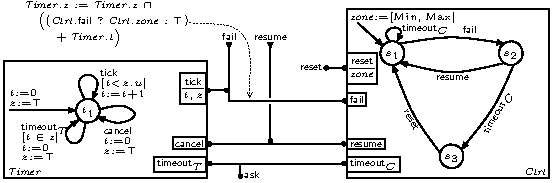
\includegraphics[width=0.9\columnwidth]{BIPspec-ArchFailureTimerMax-v4}
  \caption{The BIP specification of the Failure Monitor architecture}
  \label{fig:schema:ArchFailure:BIP}
\end{figure}



Transitions are labelled with ports of the
corresponding components, Boolean guards and update assignments on local
variables.  \Eg[,] the loop transition $\tstate{0}
\goesto{\PortTick, \GuardTick[], \TimerUpd[]} \tstate{0}$. % in the
%component $\NameTimer$ is labeled by the port $\PortTick$, the associated guarg and variable update. 
% It can be
%fired only when the current value of the local variable $t$ is less
%than $z.u$.
%%% , where $z = [l, u]$ is a local variable representing an
%%% interval
%Upon firing, this transition increments the value of $t$ by $1$.  
The
guards and update assignments of the transitions of $\NameCtrl$ are
omitted. By default, an omitted guard is  $\true$ and an omitted assignment is empty {\noop}.  
%\noteLH{It looks like Max is in zone, I do not understand}
%
Clearly, all guards and update assignments are monotonic.

%% \todoSBin{Speak of guard monotonicity}

\begin{definition}[Component semantics]
  \label{defn:comp:semantics}
  The \emph{semantics} of a component $B = \tuple{Q, q^0, V,
  \val{0}{}, P, \export, \goesto{}}$ is %% given by
  the LTS denoted $\semopen{B} = \tuple{S,
  s^0, \goesto{}}$, where $S = Q \times \valuations{V}$, $s^0 =
  \tuple{q^0, \val{0}{}}$ and $\goesto{}$ is the minimal transition
  relation satisfying the rule
  %
  \begin{equation}
    \label{eq:comp:semantics}
    \infer{
      q \goesto{a, g, u} q'
      \and
      \val{}{} \models g
      \and
      \val[\primeit]{}{} = \tilde{\val{}{}}[u]
      \and
      \valdiff{\val{}{}}{\tilde{\val{}{}}} \subseteq \export(a)
    }{
      (q, \val{}{}) \goesto{a,\tilde{\val{}{}}} (q', \val[\primeit]{}{})
    }
    \,.
  \end{equation}
  %
  %% \todoSB{Do we actually need this?}\todoLH{I agree: I do not think we need this}
  %% \hl{The \emph{closed semantics} of $B$ is given by the LTS denoted
  %% $\semclosed{B} \bydef{=}\reachable{\semopen{B}}$, comprising
  %% only the reachable states of $\semopen{B}$.}
\end{definition}

The use of the intermediate valuation $\tilde{\val{}{}}$ in the
conclusion and the third premise of  \eq{comp:semantics}
allows some  variables to get new values before the
transition is  fired.  Thus the component is \emph{open}
to the exchange of data with its environment.  However, the
fourth premise  states that only the variables exported through the ports participating to the interaction can be affected by the data transfer.
%restricts the set of
%variables that can be affected by such data transfer to those
%that are exported through the ports participating in the
%interaction.

\begin{definition}[Interaction model]
  \label{defn:im}
  For a finite set of component interfaces $(V_i, P_i,
  \export[i])^{i \in I}$, such that all $P_i$ and all $V_i$ are
  pairwise disjoint, %% \ie $\forall i \neq j,\ P_i \cap P_j = V_i \cap
  %% V_j = \emptyset$. 
  let $P = \bigcup_{i \in I} P_i$, $V = \bigcup_{i
    \in I} V_i$ and $\export : P \rightarrow 2^V$ such that, for any
  $p \in P_i$, $\export(p) = \export[i](p)$. 
%
  %% \noteSB{Updated this}\hl{and $V_a \bydef{=} \bigcup_{i \in
  %%   \supp{a}} \export[i](a \cap P_i)$ the set of component
  %% variables exported through $a$.}

  An \emph{interaction model over $(V, P, \export)$} is a set $\Gamma
  \subseteq 2^P \times \guards{V} \times \updates{V}$, such that,
  for any interaction $(a, g, u) \in \Gamma$, we have
  $g \in \guards{\export(a)}$ and $u \in \updates{\export(a)}$.\footnote{%
%
    Notice that this definition allows $(\emptyset, \true,
    \noop)$ and $(\emptyset, \false, \noop)$ to be included in
    $\Gamma$.
%
  }
  %% We call the set of ports $P$ the \emph{domain} of the
  %% interaction model.
\end{definition}

%% \noteLH{supp should go outside the definition}
We  
assume that all sets of components and interfaces satisfy the disjointness assumption above.
%
We call the \emph{support} of a set of ports $a \subseteq P$, denoted
$\supp{a}$, the set of the participating components. It is either the set $\setdef{i \in I}{a \cap P_i \neq
  \emptyset}$ (for $P = \bigcup_{i=1}^n P_i$) or the set $\setdef{B
  \in \cB}{a \cap P_B \neq \emptyset}$ (for $P = \bigcup_{B \in \cB}
P_B$).  The precise meaning of this notation will always be clear from
the context. 

\begin{definition}[Composition]
  \label{defn:im:sem}
  The \emph{composition} of a finite set of components $\cB = \tuple{Q_i,
  q^0_i, V_i, \val{0}{i}, P_i, \export[i], \goesto{}}^{i \in I}$ with
  the interaction model $\Gamma$ over $\tuple{V, P, \export}$
  is the component $\Gamma(\cB) = \tuple{Q, q^0, V, \val{0}{}, P,
    \export, \goesto{}}$, where
%
  $Q = \prod_{i \in I} Q_i$;
%
  $q^0 = (q_i^0)^{i \in I}$;
%
  $\val{0}{}: V \rightarrow \data$ is such that, for any $v \in
  V_i$, $\val{0}{}(v) = \val{0}{i}(v)$;
%
  and $\goesto{}$ is the minimal transition relation satisfying
  the rule
%
  \begin{gather*}
%%     \label{eq:im:empty}
%%     \infer{
%%       q_j \goesto{\emptyset, g, e} q_j'
%%       \and
%%       \forall i \neq j, q_i = q_i'
%%     }{
%%       (q_i)^{i \in I} \goesto{\emptyset, g, e} (q_i')^{i \in I}
%%     }\,,
%% %
%%     \\[0.5\baselineskip]
    \label{eq:im:sem}
%
    \infer{    
      (a, g, u) \in \Gamma
      \and
      a \neq \emptyset
      \and
      \forall i \in \supp{a}, q_i \goesto{a \cap P_i, g_i, u_i} q_i'
      \and
      \forall i \not\in \supp{a}, q_i = q_i'
%
      \\\\
      \textstyle
%
      g' = g \land \bigwedge_{i \in \supp{a}} g_i
      \and
      u' = u; u_i^{i \in \supp{a}}
    }{
      (q_i)^{i \in I} \goesto{a, g', u'} (q_i')^{i \in I}
    }\,.
  \end{gather*}
  %% \todoSBin{Add the intuitive explanation}
\end{definition}

\addSB{Intuitively, an interaction can be fired if all the involved
  components are ready to fire their corresponding transitions.  The
  other components do not change their states.  Both the interaction
  guard and those of the participating transitions must be satisfied.
  The update assignment of the interaction is executed first, followed
  by those of the components.}

Specifying interaction models as sets of sets of ports is not
practical due to their potentially exponential size.  An algebra of
connectors was introduced in \cite{BliSif08-acp-tc} in order to
structure interactions in BIP models.
Connectors are hierarchical, tree-like structures with component ports
at the leaves.  They define sets of interactions, based on the
attributes of the nodes, which may be either \emph{trigger}
(triangles in \fig{schema:ArchFailure:BIP}) or \emph{synchron}
(bullets in \fig{schema:ArchFailure:BIP}).
%
If all sub-connectors of a connector are synchrons, then an
interaction is allowed by the connector only if each subconnector
can contribute.
%
If at least one of the sub-connectors is a trigger, then any
interaction consisting of contributions of any set of sub-connectors
\emph{involving at least one of the triggers} is allowed.
%
The interaction model is defined as the set of all interactions
allowed by at least one of the connectors.
%% The composition semantics of BIP systems consists in
%% firing exactly one interaction, enabled through at least one of the
%% top-level connectors, at each execution round.

For instance, the connector {\NameTimer.\PortTick
  \trigsynch (\PortFail \trigsynch \NameCtrl.\PortFail)} of \fig{schema:ArchFailure:BIP} is a
two-level hierarchical connector.  In the  subconnector
{\PortFail \trigsynch \NameCtrl.\PortFail}, the port {\PortFail} is a
trigger, whereas {\NameCtrl.\PortFail} is a synchron.  This
subconnector allows two interactions: $\{\PortFail\}$ and $\listset{\NameCtrl.\PortFail, \PortFail}$.  Similarly, at the top level,
{\NameTimer.\PortTick} is a trigger, and the 
subconnector is a synchron. 
% Hence, the overall connector allows the
%interaction involving only one port {\NameTimer.\PortTick}\footnote{%
%%
%  Such interactions are called \emph{singleton interactions}.
%%
%} and any interaction involving both {\NameTimer.\PortTick} and
%\emph{some} interaction of the second-level subconnector.  
%Combining
%the two levels we can see that t
The entire connector defines the
following three interactions (observe that $\topinterval +
\NameTimer.t = \topinterval$ and $\NameTimer.z \cap \topinterval =
\NameTimer.z$):
%
%\begin{gather*}
$  \bigl(\{\NameTimer.\PortTick\},
  \true, \emptyset\bigr)
  %% \NameTimer.z := \NameTimer.z\bigr)
 $,
$  \bigl(\{\PortFail, \NameTimer.\PortTick\},
  \true, \emptyset\bigr)$
  %% \NameTimer.z := \NameTimer.z\bigr)
  ,
$
  \bigl(\{\NameCtrl.\PortFail, \PortFail, \NameTimer.\PortTick \},
  \true,
  \NameTimer.z := \NameTimer.z \cap (\NameCtrl.\mathit{zone} + \NameTimer.t)\bigr)
$
%  .
%\end{gather*}
%% \begin{align*}
%%   \bigl(\{\NameTimer.\PortTick\}&,
%%   \true, 
%%   \NameTimer.z := \NameTimer.z\bigr)
%%   \,,\\
%%   \bigl(\{\PortFail, \NameTimer.\PortTick\}&,
%%   \true,
%%   \NameTimer.z := \NameTimer.z\bigr)
%%   \,,\\
%%   \bigl(\{\NameCtrl.\PortFail, \PortFail, \NameTimer.\PortTick \}&,
%%   \true,
%%   \NameTimer.z := \NameTimer.z \cap (\NameCtrl.\mathit{zone} + \NameTimer.t)\bigr)
%%   \,.
%% \end{align*}

%% \todoSB{Update this}
%% \hl{For instance, in \fig{schema:ArchFailure:BIP}, the two ports
%% $\NameTimer.\PortStart$ and $\NameCtrl.\PortFail$ are always
%% synchronised, since they belong to exactly one binary sub-connector,
%% where they are both synchrons.  In particular, this means that
%% whenever the transition \cstate{0} \goesto{\PortFail} \cstate{1} is
%% fired, so is the transition \tstate{0} \goesto{\PortStart,
%%   \TimerInit[]} \tstate{1}, initialising the timer.  The binary
%% connector $\NameTimer.\PortStart \twosynch
%% \NameCtrl.\PortFail$ is a sub-connector of a hierarchical connector,
%% where the port $\NameOprnd.\PortFail$ is a trigger.  Thus, the above
%% interaction can only happen together with $\NameOprnd.\PortFail$,
%% forming a ternary interaction.  On the contrary, being a trigger, the
%% port $\NameOprnd.\PortFail$ can fire alone, forming a singleton
%% interaction.}

%% \todoSBin{Speak of data transfer}

%% \todoSBin{Provide the interaction model}

\addSB{In addition to interaction models, BIP relies on 
  \emph{priority models} that impose  a strict partial order on
  interactions.  Formal definitions are provided in \app{arch:appendix}.  Intuitively, an interaction can be fired only if all
  the higher-priority interactions available in the current state are
  disabled by their respective guards.
%
In the next sections, we will implicitly assume application of the  \emph{maximal
  progress} priority $\mu$, where $(a, g, u) \prec_\mu (b, h, w)$ iff  $a \subset b$ and $a \neq b$.  For instance, the
port $\NameTimer.\PortTick$ will never fire alone if the port $\PortFail$ is also enabled.
In \secn{conclusion}, we discuss the generalisation of the
obtained results to other priority models.
}
%% Below, we will assume that the maximal progress priority $\mu$ is
%% applied after each composition with an interaction model.

%% Finally, \emph{priorities}\mdash defined by a strict partial order on
%% the set of possible interactions\mdash narrow the choice among the
%% enabled interactions at any given round.  The default priority is the
%% so-called \emph{maximal progress}, whereby among any two interactions
%% $a \subset b$ (as sets of ports), $b$ has higher priority than $a$.

%% In our running example, under the maximal progress priority, the
%% port $\NameTimer.\PortTick$ will never fire alone in a global state,
%% where the \noteSB{This turns out to be the first use of the word. I am tempted to pretend I did not notice.}\hl{dangling} port $\PortFail$ is also enabled. 

%% Adding priorities $\NameOprnd.\PortFinish < \NameCtrl.\PortReset$ and
%% $\NameOprnd.\PortFinish < \NameOprnd.\PortResume$, ensures that, after
%% a failure, the operation performed by $\NameOprnd$ cannot finish
%% unless it is explicitly resumed or the system is reset.

%% \begin{note}
%%   \label{rem:maxprogress}
%% \end{note}


%% %****************************************************************
%% \subsection{Running example: Failure Monitor architecture}
%% \label{secn:failure-monitor}

%\noteLH{Ludo ou simon: essayer de remonter la description generique en debut de section}

%****************************************************************
\subsubsection{Architectures}
\label{secn:archi}

Architectures are partial BIP models, with \emph{dangling}
ports that serve as placeholders for the eventual connection with
 \emph{operand} components.

%% Contrary to standard BIP models, architectures comprise one or several
%% \emph{operand} components, whereof only the set of \emph{ports} is
%% given.  Here, the operand component is $\NameOprnd$ and its interface
%% consists of the ports $\PortFinish$, $\PortResume$ and $\PortFail$.

%% Application of the Failure Monitor architecture ensures that, whenever
%% a failure is registered in the operand component, the system will be
%% reset, unless a resumption is registered within $\mathrm{Max}$ time
%% units (more details in Sect.~\ref{section:resultOA}).

%% \noteLHin{should we say that always epsilon C is the epsilon of C?}

\begin{definition}[Architecture]
  \label{defn:arch}
  An \emph{architecture} is a tuple $A = \tuple{\cC, V_A, P_A,
    \export[A], \Gamma}$, where\vspace{-1.5ex}
  \begin{itemize}
\item
  $\cC$ is a finite set of \emph{coordinating components},
  %% with pairwise disjoint sets of ports and variables,
  such that
  $\bigcup_{C \in \cC} P_C \subseteq P_A$ and
  $\bigcup_{C \in \cC} V_C \subseteq V_A$;
%
  ports in $P_A \setminus \bigcup_{C \in \cC} P_C$, which do not
  belong to any of the coordinating components are called
  \emph{dangling};

\item
  $\export[A] : P_A \rightarrow 2^{V_A}$ is an export function, such
  that $\export[A](p) = \export[C](p)$, for any $C \in \cC$ and $p \in
  P_C$ and $\export[A](p) \subseteq V_A \setminus \bigcup_{C \in \cC}
  V_C$ for any dangling port $p$; and

\item
  $\Gamma \subseteq 2^{P_A} \times \guards{V_A} \times \updates{V_A}$
  is an interaction model over $(V_A, P_A, \export[A])$.
  \end{itemize}

\end{definition}

\begin{definition}[Application of an architecture]
  \label{defn:arch:application}
  Let $A = \tuple{\cC, V_A, P_A, \export[A], \Gamma}$ be an architecture and let $\cB$
  be a set of components, such that
  $V_A \subseteq V \bydef{=} \bigcup_{B \in \cB \cup \cC} V_B$,
  $P_A \subseteq P \bydef{=} \bigcup_{B \in \cB \cup \cC} P_B$
%
  %% \begin{align}
  %%   \bigcup_{B \in \cB} V_B \cap \bigcup_{C \in \cC} V_C = \emptyset\,,
  %%   &&
  %%   V_A \subseteq V \bydef{=} \bigcup_{B \in \cB \cup \cC} V_B\,,
  %%   \\
  %%   \bigcup_{B \in \cB} P_B \cap \bigcup_{C \in \cC} P_C = \emptyset\,,
  %%   &&
  %%   P_A \subseteq P \bydef{=} \bigcup_{B \in \cB \cup \cC} P_B\,,
  %% \end{align}
%
  and $\export[A](p) = V_A \cap \export[B](p)$, for any $B \in \cB$
  and $p \in P_A \cap P_B$.
%
  The \emph{application of the architecture $A$ to the set of
  components $\cB$} is the component $ A(\cB) \bydef{=}
  \mu\bigl((\IMextend{\Gamma}{P})(\cC \cup \cB)\bigr)$, where
%
  $\IMextend{\Gamma}{P} \bydef{=}
  \bsetdef{
    (a, g, u)
  }{
    a \subseteq P,
    (a \cap P_A, g, u) \in \Gamma
  }$
  is
  %% is the \emph{extension} of the interaction
  %% model $\Gamma$ to the set of ports $P$, \ie
  the interaction model
  over $\tuple{V, P, \export[A] \cup  \bigcup_{B \in \cB}\export[B]}$ %, with  $\export(p) = \export[C](p) \cup  \export[B](p)$
%\vspace{-1.5ex}
%  \[
%  \export(p) = 
%  \begin{cases}
%    \export[C](p), & \text{for all } C \in \cC, p \in P_C,
%    \\
%    \export[B](p), & \text{for all } B \in \cB, p \in P_B,
%  \end{cases}
%  \]
%% defined by \noteLH{looks like this also depends on Pa}
%% %
%%   \noteSB{It does, indeed.  To be completely rigorous, I could replace
%%     this with something like $\Gamma\uparrow_{P_A}^P$ but this is
%%     quite heavy and the dependency is already implicit from the fact
%%     that $\Gamma$ is defined on $P_A$}
%% %
%%   \noteSB{Which one of \eq{im:extension} and \eq{im:extension1} is
%%     more intuitive?}
%
  %% \begin{align}
  %%   \label{eq:im:extension}
  %%   \IMextend{\Gamma}{P} &\bydef{=}
  %%   \bsetdef{
  %%     (a \cup a', g, e)
  %%   }{
  %%     (a, g, e) \in \Gamma, a' \subseteq P \setminus P_A
  %%   }
  %%   \\
  %%   \label{eq:im:extension1}
  %%   &= 
  %%   \bsetdef{
  %%     (a, g, e)
  %%   }{
  %%     a \subseteq P,
  %%     (a \cap P_A, g, e) \in \Gamma
  %%   }
  %% \end{align}
%
  and $\mu(\dots)$ denotes the application of maximal progress.
\end{definition}

%% \todoSBin{Define equivalence $\arequiv$?}

An architecture $A$ enforces coordination constraints on the
components in $\cB$.  The interface $(V_A, P_A, \export[A])$ of an
architecture $A$ contains all ports of the coordinating
components $\cC$ and the dangling ports, which must belong to
the components in $\cB$.  In the application $A(\cB)$, the ports
belonging to $P_A$ can only participate in the interactions
defined by the interaction model $\Gamma$ of $A$.  Ports which do
not belong to $P_A$ are not restricted and can participate in any
interaction.  %% In particular, they can join the interactions in
%% $\Gamma$ (see \defn{arch:application}).  If the interface of the
%% architecture covers all ports of the system, \ie $P = P_A$, we
%% have $P\setminus P_A = \emptyset$ and the only interactions
%% allowed in $A(\cB)$ are those belonging to $\Gamma$.  Notice also
%% that the restrictions imposed by \defn{arch:application} on the
%% set of operand components $\cB$ ensure that an interaction in
%% $\IMextend{\Gamma}{P}$ can only refer to variables of the
%% participating components.
%
%% Finally, 
The definition of $\IMextend{\Gamma}{P}$ requires that
an interaction from $\Gamma$ be involved in every interaction
belonging to $\IMextend{\Gamma}{P}$.  To allow the ports from $P
\setminus P_A$ to be fired independently in $A(\cB)$, one must
have $(\emptyset, \true, \noop) \in \Gamma$.  

In our running example, there are four dangling ports.  Intuitively, the
architecture monitors the activation of the dangling port {\PortFail}, then
waits for a period comprised between $\mathrm{Min}$ and $\mathrm{Max}$
and, unless {\PortResume} is activated, asks for a system reset
through an invocation of the dangling port {\PortAsk}.

\begin{definition}[Composition of architectures]
  \label{defn:arch:composition}
  Let $A_i = \tuple{\cC_i, V_{A_i}, P_{A_i}, \export[A_i], \Gamma_i}$, for $i = 1,2$,
  be two architectures.  The \emph{composition} of $A_1$ and
  $A_2$ is the architecture $A_1 \arcomp A_2 = \tuple{\cC_1 \cup \cC_2,
  V_{A_1} \cup V_{A_2}, P_{A_1} \cup P_{A_2}, \export[A_1] \cup \export[A_2], \Gamma}$, where\vspace{-1ex}
%
  \begin{equation}
    \label{eq:arch:composition}
    \Gamma = \bsetdef{
      (a, g^1 \land g^2, u^1 \expmix u^2) 
    }{
      (a \cap P_{A_i}, g^i, u^i) \in \Gamma_i,
      \text{ for } i = 1,2
    }
    \,.
  \end{equation}
\end{definition}

%\begin{proposition}[Properties of $\arcomp$]
%  \label{prop:arcomp:nice}
  %% Architecture composition
$\arcomp$ is associative and commutative.
  %%; it is idempotent if all coordinating components
  %% are deterministic; $A_{id} = \bigl(\emptyset, \emptyset,
  %% \emptyset, \emptyset, \{(\emptyset, \true, \noop)\}\bigr)$ is its neutral element, \ie for
  %% any architecture $A$, we have $A \oplus A_{id} \arequiv A$.
  %% Furthermore, for any component $B$, we have $A_{id}(B) = \mu(B)$.
%\end{proposition}
%
%% \begin{proof}[Sketch of the proof]
%%   %% Commutativity and associativity 
%%   Follows from the corresponding
%%   properties of set union, Boolean conjunction and
%%   semilattice meet.
%% %
%% %% \todoLH{Check when equivalence is defined}
%% %%   Suppose we have two architectures $A \arequiv A'$.  This does not
%% %%   necessarily mean that their sets of coordinating components
%% %%   coincide.  However, if all the involved coordinating components
%% %%   are deterministic, then, in any state of $(A \arcomp A')(\cB)$,
%% %%   both architectures will impose the same restrictions, enabling
%% %%   the same interactions between the coordinating and operand
%% %%   components.  Hence, we have $(A \arcomp A')(\cB) = A(\cB) =
%% %%   A'(\cB)$.  Since this holds for any set of components $\cB$, we
%% %%   conclude that $A \arcomp A' \arequiv A \arequiv A'$.
%% %% %
%% %%   The properties of $A_{id}$ follow immediately from the
%% %%   definitions of architecture application and composition.
%% \end{proof}
%% The last statement of \prop{arcomp:nice} highlights a subtle point:
%% $A_{id}$ is the neutral element of the $\arcomp$ operator\mdash it is
%% not the identity operator on components.
%****************************************************************
%\subsubsection{Preservation of safety properties}
%\label{secn:safety}
For a component $B$, we denote $S_{\semopen{B}}$ and
$s^0_{\semopen{B}}$ the corresponding constituents of
$\semopen{B}$ (see Definition~\ref{defn:comp:semantics}).

\begin{definition}[Properties]
  \label{defn:property}
  Let $B$ be a component.  A \emph{(safety) property} 
  of $B$ is a predicate $\Phi$ on
  $S_{\semopen{B}}$, such that $\bigl((q,
  \val{}{}) \models \Phi\bigr) \land (\val[\primeit]{}{} \order
  \val{}{})$ implies $(q, \val[\primeit]{}{}) \models \Phi$.
  %% ,
  %% where we write $(q, \val{}{}) \models \Phi$ iff $\Phi(q,
  %% \val{}{}) = \true$.
  A property $\Phi$ is \emph{initial} if
  $s^0_{\semopen{B}} \models \Phi$.
  %% \todoSB{Do we need this?}\hl{;
  %% it is \emph{reachable} iff there exists a possibly empty path
  %% $s^0_{\semopen{B}} \goesto{a^1, \val{1}{}} s^1 \goesto{a^2,
  %%   \val{2}{}} \cdots \goesto{a^n, \val{n}{}} s^n$, such that
  %% $s^n \models \Phi$}.
\end{definition}

\label{property:reset}
Although we define properties as state predicates, any
appropriate logic can be used to specify them.  For instance, the
property \addSB{\emph{``There is always a possibility to reset the system
  after a single failure''} (\ie without
  additional failures having to occur in the meantime)} enforced by the
Failure Monitor architecture can be specified using CTL as \noteSB{Removed $\lnot \PortResume$, because not needed \emph{and} could not reformulate nicely in English.}\addSB{$\AG
\bigl(\PortFail \rightarrow \EX \EU[]{\lnot \PortFail}{
  \PortReset}\bigr)$}.  Additional properties are provided in
\app{properties}.
%% \todoSB{Cite the original paper somewhere.}
An architecture enforces
its characteristic property on  its operand components.
From this point of view, the set of coordinating components is
not relevant, neither are their states.  Thus, 
properties enforced by architectures only involve
the unrestricted composition of the operands:

\begin{definition}[Enforcing properties]
  \label{defn:enforce}
  Let $A = \tuple{\cC, P_A, V_A, \export[A], \Gamma}$ be an architecture; let $\cB$
  be a set of components and $\Phi$ an initial property of
  their parallel composition $\Gamma_{\|}(\cB)$,
  with $\Gamma_{\|} = \setdef{(a,\true,\emptyset)}{a \subseteq \bigcup_{B \in \cB} P_B}$.
  We say that \emph{$A$ enforces $\Phi$ on
    $\cB$} iff, for every state $s = (s_c, s_b)$ reachable in
  $\semopen{A(\cB)}$, with 
  $s_c \in \prod_{C \in \cC} S_{\semopen{C}}$ and
  $s_b \in \prod_{B \in \cB} S_{\semopen{B}}$,
  we have $s_b \models \Phi$.
\end{definition}
In the following, when we say that an
architecture enforces some property $\Phi$, $\Phi$ is supposed to be initial for the coordinated components.
%
%According to the above definition, when we say that an
%architecture enforces some property $\Phi$, it is implicitly
%assumed that $\Phi$ is initial for the coordinated components.
%Below, we omit mentioning this explicitly.
\defn{up:compat} in \app{arch:appendix} formally defines
 \emph{upwards compatibility} that ensures property preservation when composing architectures. Informally, two architectures $A_1$ and $A_2$
are  upwards compatible iff, whenever their composition
involves the fusion of two interactions $a_1 = a \cap P_{A_1}$ and
$a_2 = a \cap P_{A_2}$ (see \eq{arch:composition}) and one, say
$a_1$, is inhibited in a given state by a larger interaction $b_1
\supset a_1$, there exists an interaction $b_2 \supseteq a_2$ that can
be fused with $b_1$ to form an interaction enabled in the same state.

\begin{theorem}[Preserving enforced properties]
  \label{thm:combining}
  Let $\cB$ be a set of components; let $A_i = \tuple{\cC_i, V_{A_i},
  P_{A_i}, \export[A_i], \Gamma_i}$, for $i = 1,2$, be two upwards compatible architectures
  enforcing on $\cB$ the properties $\Phi_1$ and $\Phi_2$
  respectively.  The composition $A_1 \arcomp A_2$ enforces on
  $\cB$ the property $\Phi_1 \land \Phi_2$.
\end{theorem}

%****************************************************************

%****************************************************************

\section{Encoding of architectures into open pNets}
\label{secn:encoding}

We  define the encoding of BIP architectures into pNets by
associating to each architecture $A = \tuple{\cC, V_A, P_A,
  \export[A], \Gamma}$ with $C = \tuple{Q_C, q^0_C, V_C, \val{0}{C},
  P_C, \export[C], \goesto{}}$, for each $C \in \cC$, \emph{and a
  partition $\partition \subseteq 2^{P_A}$ of its dangling ports} (\ie
$\biguplus_{D \in \partition} D = P_A \setminus \bigcup_{C \in \cC}
P_C$), the corresponding pNet $\nopri[A, \partition]$.
%
%% and $D_1 \cap D_2 = \emptyset$, for any two distinct $D_1, D_2
%% \in \partition$.
%
%% Notice that this addition 
%% is a matter of convenience, since one can
%% use the trivial partition $\partition \bydef{=} \{P_A \setminus \bigcup_{C
%%   \in \cC} P_C\}$.
For the sake of clarity, we define the encoding  without  any priority model.  Then, we provide a brief sketch of the
modifications necessary to encode maximal
progress (implicitly assumed).
%% %****************************************************************
%% \subsection{Encoding without the priority model}
%% \label{secn:enc:nopri}
Recall that $\Gamma$ is an interaction model over the interface
$\tuple{V_A, P_A, \export[A]}$, \ie these interface elements are
implicitly involved in the definition of $\Gamma$.
%
We define $\nopri[A, \partition] \bydef{=} \pNetTuple{(\nopri[C])^{C
    \in \cC}, \partition, \nopri[\Gamma]}$, where $\nopri[C]$ and
$\nopri[\Gamma]$ are the encodings of a coordinator $C$ and the
interaction model $\Gamma$ respectively.

\paragraph{Encoding the coordinators.}
The encoding of a coordinator $C$ is a pLTS with: 1)~an
 initial state and an   
$\init$ transition that initialises all the variables to those defined
by the initial valuation $\val{0}{C}$ of $C$, 2)~an action algebra that matches the actions of the coordinator ports but adds, an additional boolean action parameter, and also, for each exported
variable $x$, a corresponding fresh input variable $?x'$ to allow updates during interactions, 3)~pLTS transitions that reflect the original transitions of
$C$ with $\true$ as parameter and 5)~additional loop transitions marked by
$\false$.
\noteLH{enleve le 3 et integre au 2}
Formally,  $\nopri[C] \bydef{=} \pNetTuple{S, s_0, \goesto[{\nopri[C]}]{}}$, such that
%
\begin{itemize}
\item $s_0 \not\in Q_C$ is fresh and $S = Q_C \cup \{s_0\}$,
  \noteEM{En principe les $vars(s)$ devraient etre disjoints, mais je
    veux bien laisser ca sous le tapis tant qu'on n'implemente pas le codage...}
\item $\vars(s) = V_C \cup \setdef{?x'}{x \in \export[C](p), p \in a, s\goesto{a} }$, for all $s \in Q_C$, and $\vars(s_0) =
  \emptyset$,
%% \item the transition relation $\goesto[{\nopri[C]}]{}$ is defined as
%%   the union of three sets of transitions
%%   (with $\mathit{init} \bydef{=} \bigl(x := \val{0}{C}(x)\bigr)^{x \in V_C}$):
%% %
%%   \begin{multline}
%%     \label{eq:nopri:trans}
%%     {\goesto[{\nopri[C]}]{}} \bydef{=}
%%     \bsetdef{\tuple{s, a(\true), g, u, s'}}{
%%       \tuple{s, a, g, u, s'} \in \goesto{}}
%%     \\    
%%     \cup
%%     \bsetdef{\tuple{s, a(\false), \true, \noop, s}}{
%%       s \in Q_C, a \in P_C}
%%     %% \\
%%     \cup
%%     \bigl\{(s_0, \init, \true, \mathit{init}, q^0_C)\bigr\}
%%     \,.
%%   \end{multline}

\item let  $\mathit{uinit} \bydef{=} \bigl(x := \val{0}{C}(x)\bigr)^{x \in V_C}$ and,
  \noteSB{Ludo, Eric, pourriez-vous v\'erifier que cela est
    compr\'ehensible ? Ok pour moi (Eric) OK Ludo, rephrase un peu}%
  \add{for all $s \goesto{a, g, u} s'$ with $u = (x\! :=
\! e_x)^{x
    \in V}$ (with $V \!\subseteq\! V_C$),
%  
  let $u' \bydef{=}
  \bigl(x := e_x\bigr)^{x \in V \setminus \export[C](a)}
  \cup
  \bigl(x := e_x\bigl[\nicefrac{?x'}{x}\bigr]\bigr)^{x \in V \cap \export[C](a)}$,
%
  and $\export[C]'(a) \bydef{=} \setdef{?x'}{x \in \export[C](p), p \in a}$,
%
\noteEM{j'ai inverse les $\export[C]'(a), \export[C](a)$ dans les
  actions, pour etre conforme a la notation de la Def 1 page 4. }
\begin{multline*}
    {\goesto[{\nopri[C]}]{}} \bydef{=} 
    \Setdef{\Tuple{s, a\bigl(\export[C]'(a), \export[C](a),\true\bigr), g, u', s'}}{
      s \goesto{a, g, u} s'}
    \\
    {} \cup
    \Setdef{\Tuple{s, a\bigl(\export[C]'(a), \export[C](a),\false\bigr), \true, \noop, s}}{
      s \in Q_C, \exists s' \in Q_C: s' \goesto{a}}
    \\
    {} \cup \bigl\{(s_0, \init, \true, \mathit{uinit}, q^0_C)\bigr\}.
  \end{multline*}}
\end{itemize}\vspace{-3ex}

The loop transitions marked by $\false$ will be used in the encoding
of connectors.  Each BIP connector can define several interactions,
\ie ports involved in a connector need not necessarily always
participate.  On the contrary, each action in a pNet synchronisation
vector must participate in the synchronisation.  To address this
difference, we use the classical approach
where non-participation of a port in an interaction is simulated
by an additional loop transition~\cite{milner83-calculi}.

\Fig{FailureTimer:pNet} shows the encoding of the Failure Monitor
architecture, including the encodings of the two coordinators, \ie
$\nopri[\NameTimer]$ and $\nopri[\NameCtrl]$.  Notice that the
encoding in the figure is slightly optimised: some of the ports do not
have an associated Boolean value, nor the additional loop transitions.
We will explain this optimisation after we define the
encoding of the interaction model.

\begin{figure}[t]
  \centering
  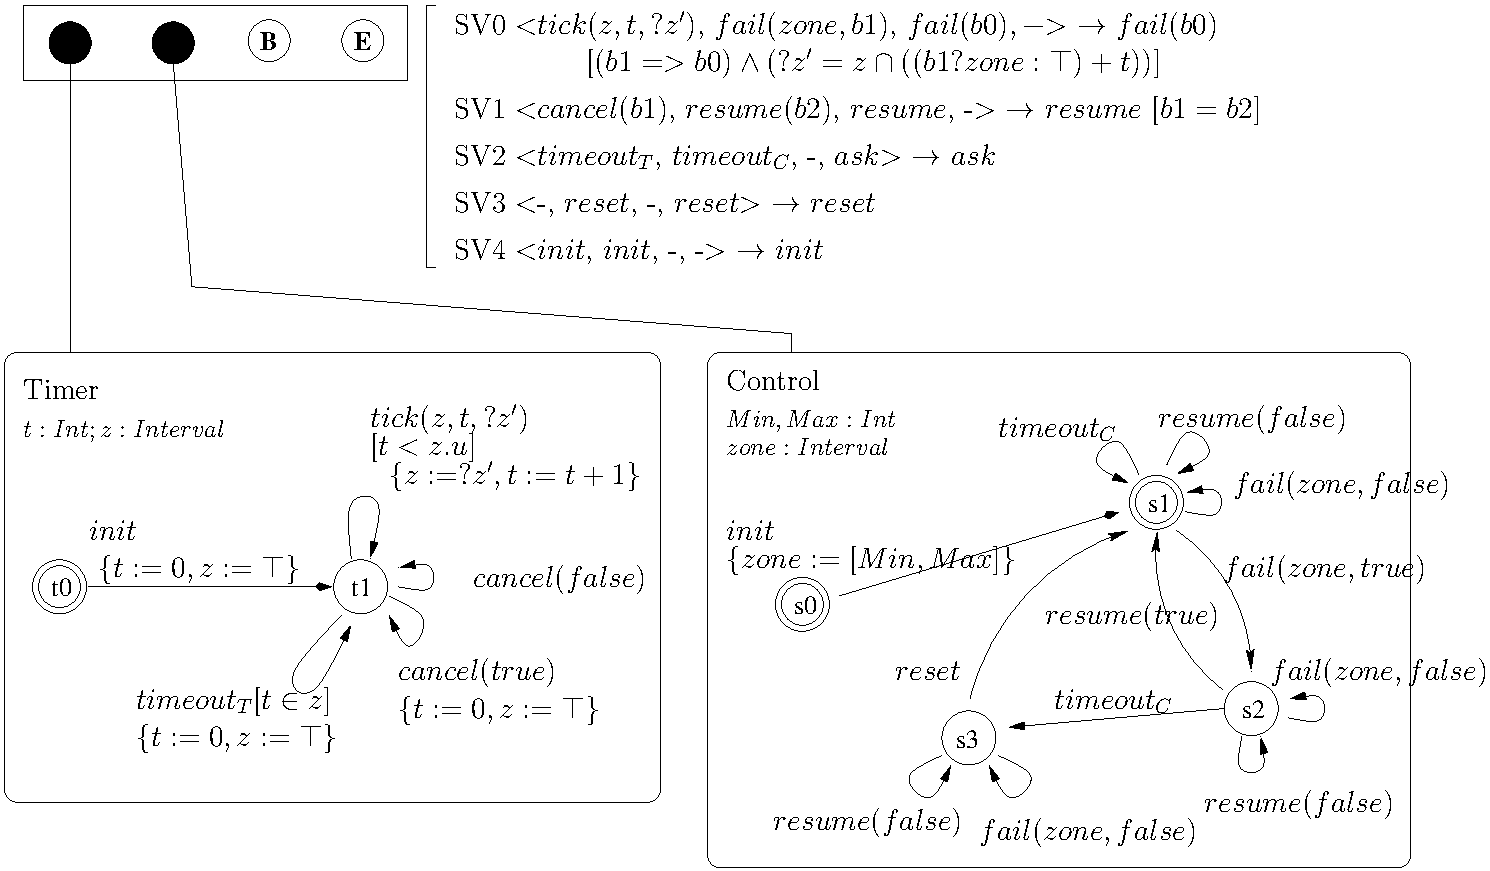
\includegraphics[width=0.9\columnwidth]{FailureTimerPNET-v4}
  \caption{The open pNET encoding the Failure Monitor architecture (\fig{schema:ArchFailure:BIP}) without the Max Progress priority model}
  \label{fig:FailureTimer:pNet}
%% %
%%   \noteSBin{The updated encoding exports more primed variables in the
%%     actions, \eg $tick(z,t,z',t')$ and $fail(zone, zone', b1)$ instead
%%     of $tick(z,t,z')$ and $fail(zone, b1)$, and SVs, \eg $\dots \land
%%     (t' = t) \land (zone' = zone)$ in the guard of SV0. Shall we
%%     update the figure to include these or, rather, explain that the
%%     figure is cleaned-out for readability?}
%
\end{figure}

%% \begin{figure*}[t]
%%   \fbox{%
%%   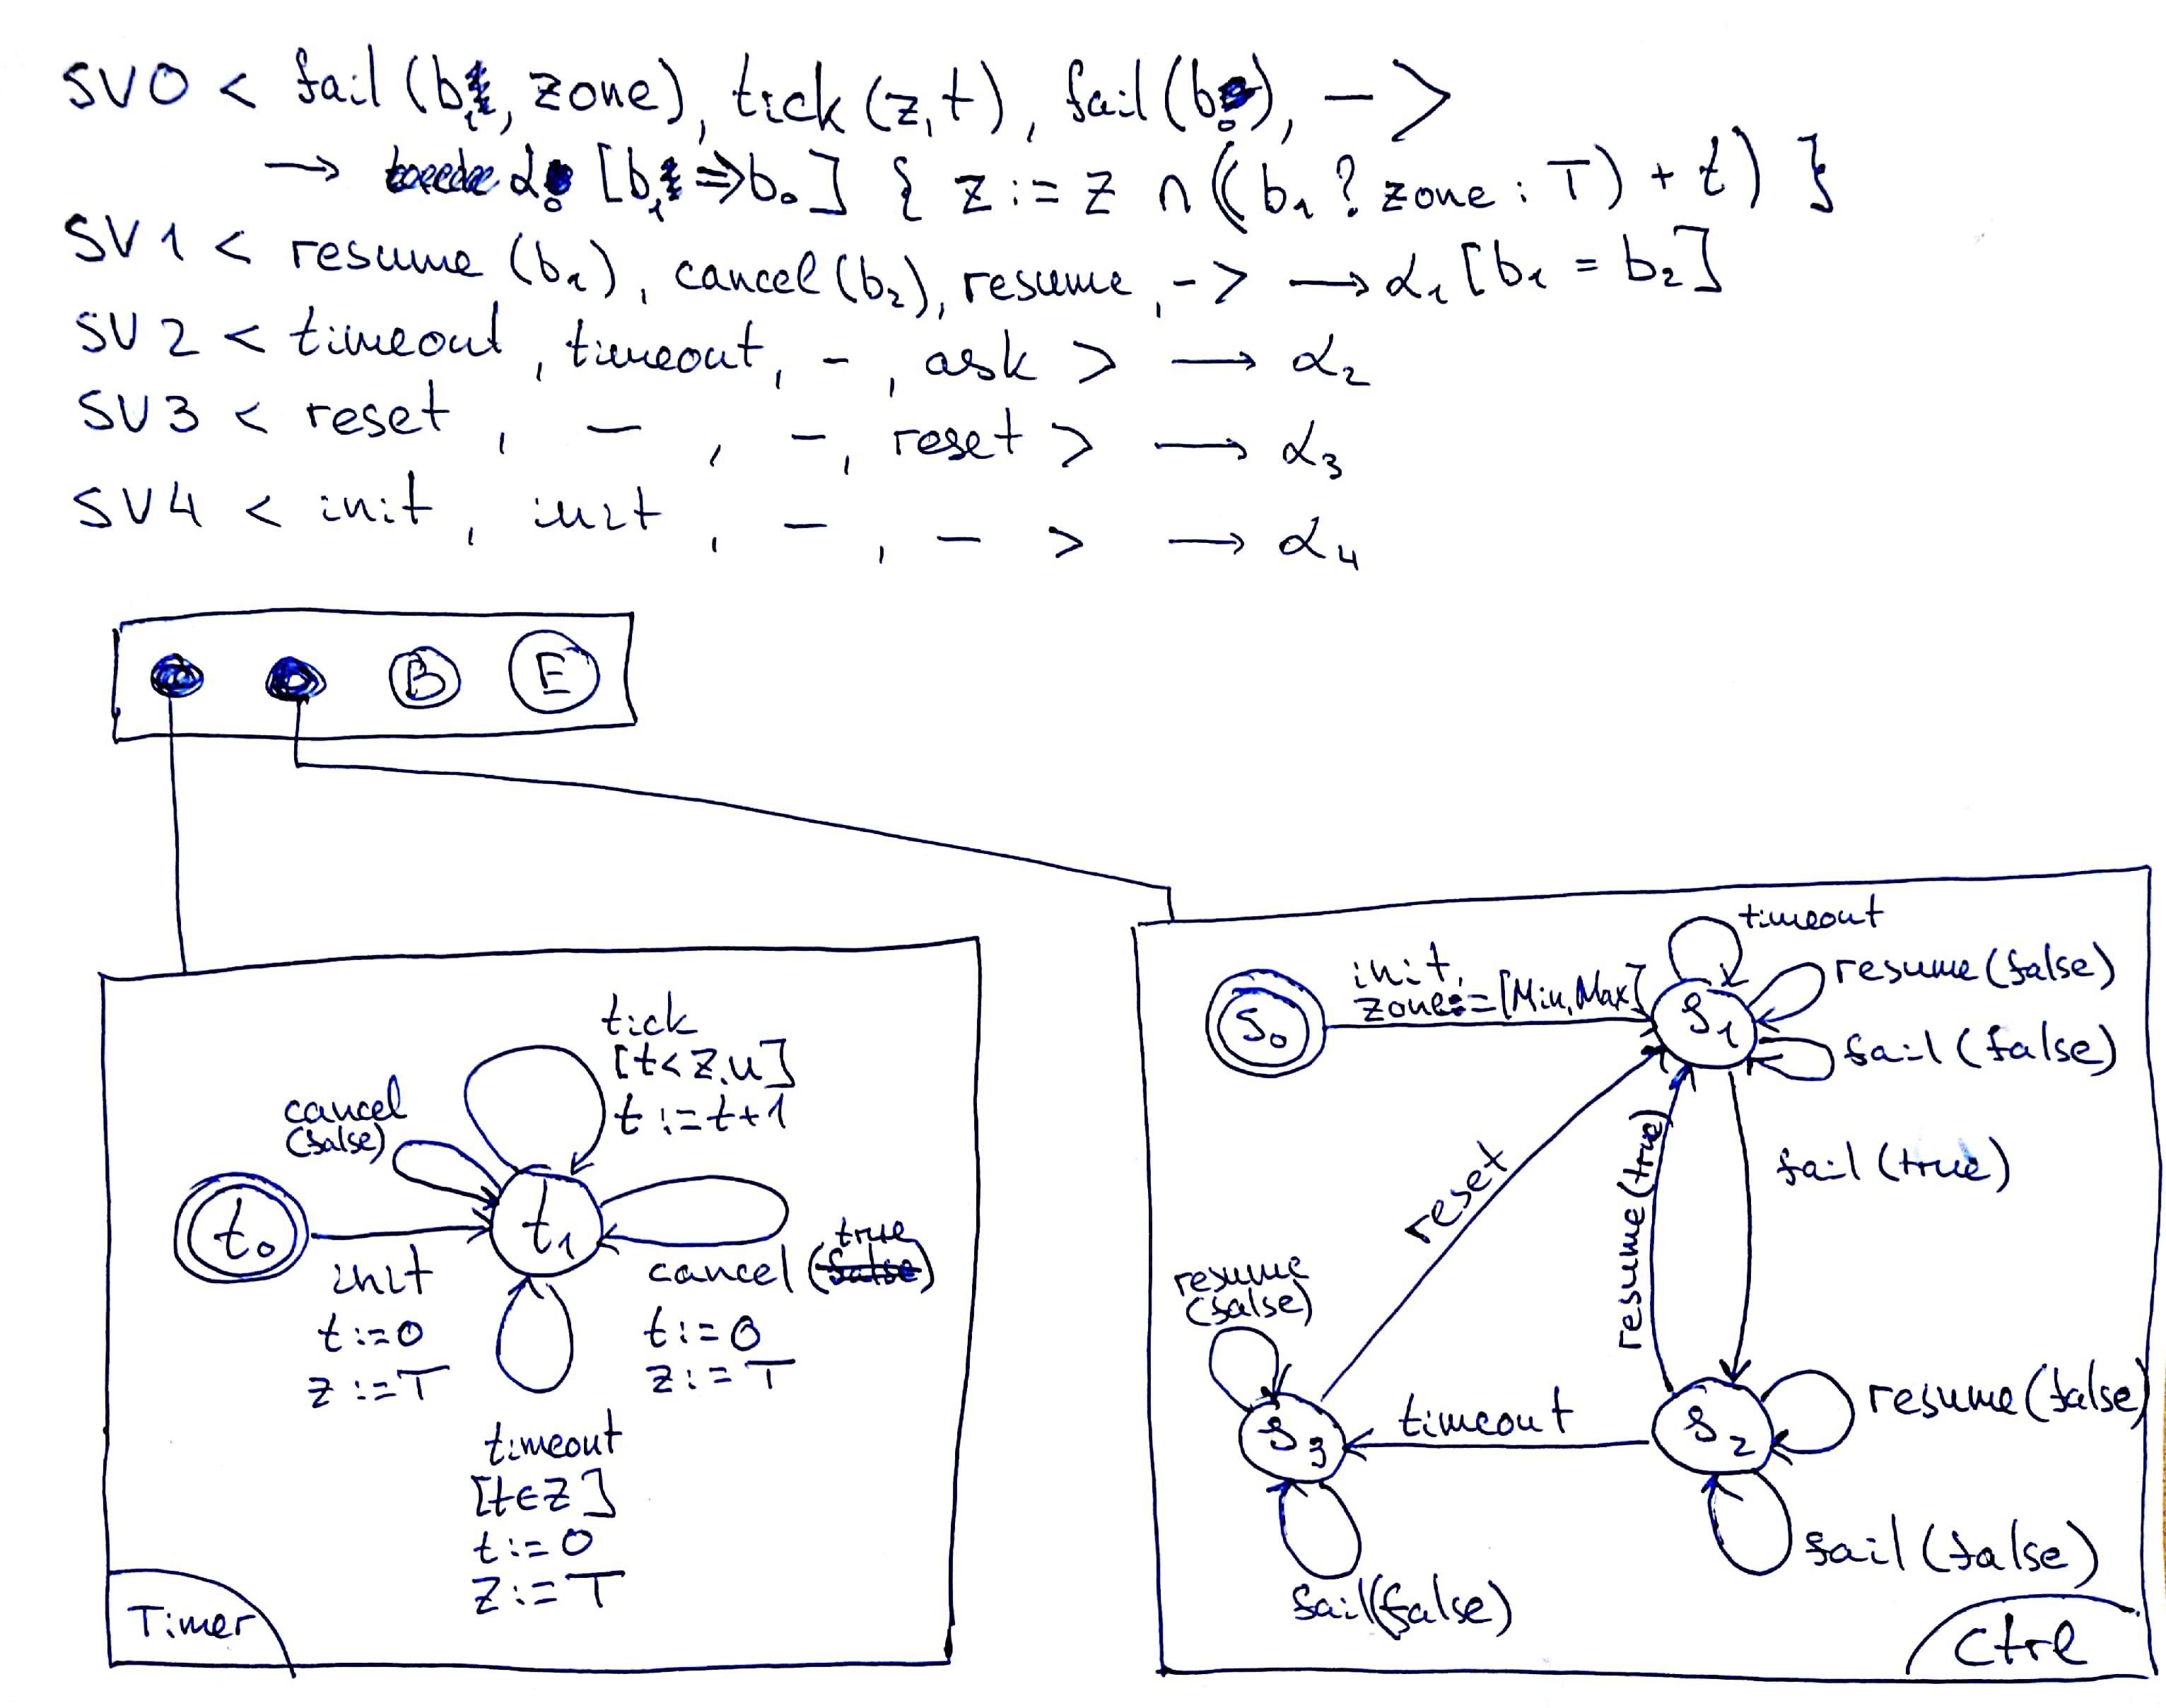
\includegraphics[width=\textwidth]{BIPspec-ArchFailureTimerMax-v4-no-pri}}
%%   \caption{Encoding of the Failure Monitor architecture
%%     (\fig{schema:ArchFailure:BIP}) as an open pNet (without the
%%     priority model) \hl{\bf (Error in the picture: First two positions in the synchronisation vectors must be transposed)}}
%%   \label{fig:enc:nopri}
%% \end{figure*}

\paragraph{Encoding the interaction model}
%% First of all, recall that $\nopri[A, \partition ] \bydef{=}
%% \pNetTuple{(\nopri[C])^{C \in \cC}, \partition, \nopri[\Gamma]}$.
%% Thus, 
The holes in $\nopri[A, \partition]$ are indexed by the elements of
the partition \partition.  For the encoding of our running example, we
take $\partition = \bigl\{\{\PortFail, \PortResume\},\{\PortAsk,
\PortReset\}\bigr\}$.  This corresponds to the intuition that the
dangling ports {\PortFail} and {\PortResume} will be provided by a 
monitored component, whereas {\PortAsk} and {\PortReset} correspond to
the actions provided by the ``environment'' (other components of the
system) that are invoked in case of a persistent failure.  As for
the encoding of the coordinators, in the synchronisation vectors of
\nopri[\Gamma], we will associate Boolean values to the actions
corresponding to these ports.

The encoding of the interaction model is based on its representation
as a set of connectors. \noteSB{%
%
%%   A legitimate question is whether we actually need to do this,
%%   instead of listing explicitly the individual interactions, then
%%   associating a synchronisation vector to each one of them?  One of
%%   the factors is the encoding pNets$\rightarrow$SAT: is it better to
%%   have more or fewer SVs if the price is additional Boolean variables?
%%   The other factor might be the facility of maximal progress
%%   encoding\mdash TBC.  Traceability.  Anything else?\newline
%%   \hl{UPDATE: Maximal progress encoding requires this!}
%% %
} Indeed, as illustrated by the Failure Monitor architecture in
\fig{schema:ArchFailure:BIP}, each connector can define several
allowed interactions, depending on its hierarchical structure and the
use of synchrons and triggers.

\addSB{We encode all interactions of a connector in one synchronisation vector.  This will allow us to also encode the maximal progress priority model.}
We use
the additional Boolean values associated to each port by the encoding
of coordinator components.  For example, observe that the three ports in 
the connector
{\NameTimer.\PortTick
  \trigsynch (\PortFail \trigsynch \NameCtrl.\PortFail)}
form a ``causality chain'': {\NameCtrl.\PortFail} can only
participate in an interaction if the dangling port {\PortFail}
participates, which in turn can only happen if
{\NameTimer.\PortTick} does so.  These dependencies can be rewritten
as Boolean implications $\NameCtrl.\PortFail \Rightarrow \PortFail$
and $\PortFail \Rightarrow \NameTimer.\PortTick$.
%
The conjunction of these two implications can be used as a guard for
the synchronisation vector encoding this connector.

Within the scope of this connector, the port {\NameTimer.\PortTick}
participates in all interactions.
%
Furthermore, it is not involved in any other
connector.  Hence, the loop transition in \nopri[\NameTimer]
labelled by $\PortTick(\false)$ can never be taken and, therefore, can
be removed from the encoding.  Since only the transition
labelled by $\PortTick(\true)$ is ever taken, 
%
the
implication $\PortFail \Rightarrow \NameTimer.\PortTick$ is a tautology and can also be discarded.

We obtain the
synchronisation vector SV0 shown in \fig{FailureTimer:pNet}, where $b0$ and
$b1$ are the Boolean values associated to the actions encoding the
ports {\PortFail} and {\NameCtrl.\PortFail}.
The guard $b_1 \Rightarrow b_0$ encodes the causal
relation between ports {\NameCtrl.\PortFail} and {\PortFail}.  Notice
that, in our encoding, all three ports are present in the
synchronisation vector.  \Fig{FailureTimer:pNet} shows
the four synchronisation vectors SV0\ndash SV3 corresponding to the
connectors in \fig{schema:ArchFailure:BIP} and an additional vector
SV4, synchronising the {\init} transitions of the two pLTSs.

\addSB{In the general encoding, the global actions of the
  synchronisation vectors should be fresh action names.  However, for
  the properties considered in our case study, we only need to exhibit
  the actions of the holes.  Furthermore, each synchronisation vector
  involves at most one such action.  This allows us to reuse them as
  the global actions of the synchronisation vectors, simplifying the
  translation of properties to be verified (\cf \app{properties}).}
  
The general case encoding relies on the causal semantics of the
algebra of BIP connectors \cite{BliSif10-causal-fmsd}.  Disregarding
the variables and data transfer, the Algebra of Connectors $\ac(P)$
\cite{BliSif07-acp-emsoft} provides a syntactic notation for the BIP
connectors.  The causal semantics of the connectors, given in terms of
the Algebra of Causal Interaction Trees $\ct(P)$, explicitates the
causal dependencies discussed above through an encoding mapping
$\tau: \ac(P) \rightarrow \ct(P)$.  Another mapping $R: \ct(P)
\rightarrow \cru(P)$ encodes causal interaction trees into systems of
causal rules, which are Boolean implications similar to the ones in
the example above.  We briefly summarise the key definitions and
results in \app{algebras}.  The $\ac(P)$, $\ct(P)$ and $\cru(P)$
representations of the connectors in \fig{schema:ArchFailure:BIP} are
shown in \tab{connectors} (elements shown in red can be removed for
simplification as described in the example above).

\begin{table}[t]
  \caption{Algebraic representations of the connectors in \fig{schema:ArchFailure:BIP} (see \app{algebras})}
  \label{tab:connectors}
  \resizebox{\columnwidth}{!}{%
  \begin{tabular}{@{}c|c|c@{}}
    \hline {\bf Connector} & {\bf Causal Interaction Tree} & {\bf
      System of Causal Rules}
    \\\hline    
%
    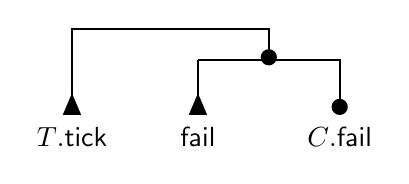
\begin{tikzpicture}[shorten >=1pt,node distance=.7cm,>=stealth']

      \node(caa) {}; % node distance=5cm [right of=start]
      \node[node distance=1cm] (cb) [below of=caa]{\PortFail};
      \node[node distance=1.8cm] (cc) [right of=cb]{\NameCtrl.\PortFail};
      \node[node distance=1.6cm] (ca) [left of=cb]{\NameTimer.\PortTick};

      \draw [style=-*, thick, black] ($(caa.south)+(0,.1cm)$) -- ++(right:.5cm) -| (cc.north);
      \draw [style=-triangle 45 reversed, thick, black]  ($(caa.south)+(0,.1cm)$) -| (cb.north);
      \draw [style=-*, thick, black] ($(caa.south)+(0,.5cm)$) -- ++(right:.2cm) -| ($(caa.south)+(+.9,0cm)$);
      \draw [style=-triangle 45 reversed, thick, black]  ($(caa.south)+(0,.5cm)$) -| (ca.north);
    \end{tikzpicture}
%
    &
%
    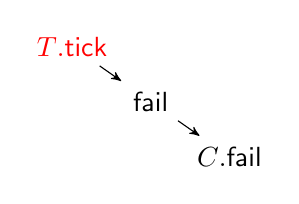
\begin{tikzpicture}[shorten >=1pt,node distance=.7cm,>=stealth'
        ,initial text=
        ,every state/.style={draw=black,thick}
        ,group/.style = {draw=black,thin,rectangle, minimum width=2.5cm}
        ,port/.style = {font=\small, minimum size=5mm}
        ,legend/.style = {font=\bf}
      ]

      \node(tick){\color{red}\NameTimer.\PortTick};
      \node[node distance=1cm](x) [right of=tick]{};
      \node(fail) [below of=x] {\PortFail};
      \node[node distance=1cm](y) [right of=fail]{};      
      \node(ctrlfail) [below of=y] {\NameCtrl.\PortFail};
      
      \draw[style=->] (tick) -> (fail);
      \draw[style=->] (fail) -> (ctrlfail);
    \end{tikzpicture}
%
    &
%
    $
    \begin{aligned}[b]
      \NameCtrl.\PortFail &\Rightarrow
      \PortFail {\color{red}{}\land \NameTimer.\PortTick}
      \\
      {\color{red}\PortFail} &{\color{red}{}\Rightarrow \NameTimer.\PortTick}
      \\
      {\color{red}\NameTimer.\PortTick} &{\color{red}{}\Rightarrow \true}
      \\
      {\color{red}\true} &{\color{red}{}\Rightarrow \NameTimer.\PortTick}

    \end{aligned}
    $
%
    \\\hline
%
    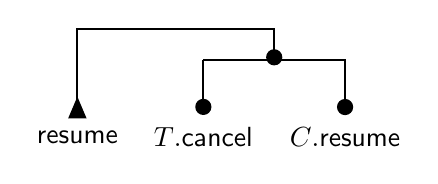
\begin{tikzpicture}[shorten >=1pt,node distance=.7cm,>=stealth']

      \node[](baa) {}; % node distance=1.8cm [right of=start]
      \node[node distance=1cm] (bb) [below of=baa]{\NameTimer.\PortCancel};
      \node[node distance=1.8cm] (bc) [right of=bb]{\NameCtrl.\PortResume};
      \node[node distance=1.6cm] (ba) [left of=bb]{\PortResume};


      \draw [style=-*, thick, black] ($(baa.south)+(0,.1cm)$) -- ++(right:.5cm) -| (bc.north);
      \draw [style=-*, thick, black]  ($(baa.south)+(0,.1cm)$) -| (bb.north);
      \draw [style=-*, thick, black] ($(baa.south)+(0,.5cm)$) -- ++(right:.2cm) -| ($(baa.south)+(+.9,0cm)$);
      \draw [style=-triangle 45 reversed, thick, black]  ($(baa.south)+(0,.5cm)$) -| (ba.north);
    \end{tikzpicture}
%
    &
%
    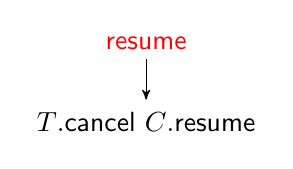
\begin{tikzpicture}[shorten >=1pt,node distance=.7cm,>=stealth'
        ,initial text=
        ,every state/.style={draw=black,thick}
        ,group/.style = {draw=black,thin,rectangle, minimum width=2.5cm}
        ,port/.style = {font=\small, minimum size=5mm}
        ,legend/.style = {font=\bf}
      ]

      \node(res){\color{red}\PortResume};
      \node[node distance=1cm](rest) [below of=res] {\NameTimer.\PortCancel\ \NameCtrl.\PortResume};
      \draw[style=->] (res) -> (rest);
    \end{tikzpicture}
%
    &
%
    $
    \begin{aligned}[b]
      \NameCtrl.\PortResume &\Rightarrow
      {\color{red}\PortResume \land{}} \NameTimer.\PortCancel
      \\
      \NameTimer.\PortCancel &\Rightarrow 
      {\color{red}\PortResume \land{}} \NameCtrl.\PortResume
      \\
      {\color{red}\PortResume} &{\color{red}{}\Rightarrow \true}
      \\
      {\color{red}\true} &{\color{red}{}\Rightarrow \PortResume}
    \end{aligned}
    $
%
    \\\hline
%
    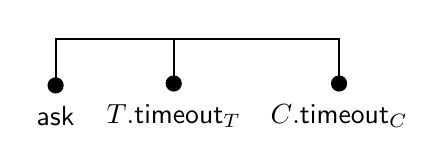
\begin{tikzpicture}[shorten >=1pt,node distance=.7cm,>=stealth']

      \node (start) {};
      \node(h4)[left of=start]{}; %, node distance=1.5cm

      \node[node distance=1cm] (ab) [below of=start] {\NameTimer.\PortTOT};
      \node[node distance=2.1cm] (ac) [right of=ab]{\NameCtrl.\PortTOC};
      \node[node distance=1.5cm] (aa) [left of=ab]{\PortAsk};

      \draw [style=-*, thick, black] ($(h4.south)+(0,.1cm)$) -- ++(right:.5cm) -| (ac.north);
      \draw [style=-*, thick, black]  ($(h4.south)+(0,.1cm)$) -| (ab.north);
      \draw [style=-*, thick, black]  ($(h4.south)+(0,.1cm)$) -| (aa.north);
    \end{tikzpicture}
%
    &
%
    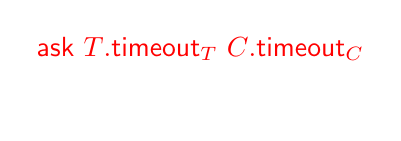
\begin{tikzpicture}[shorten >=1pt,node distance=.7cm,>=stealth']
      \node (start) {\color{red}\PortAsk\ \NameTimer.\PortTOT\ \NameCtrl.\PortTOC};
      \node()[below of=start]{};
    \end{tikzpicture}
%
    &
%
    $
    \begin{array}[b]{c@{}}
      {\color{red}
        \begin{aligned}
          \NameCtrl.\PortTOC &\Rightarrow
          \PortAsk \land \NameTimer.\PortTOT
          \\
          \NameTimer.\PortTOT &\Rightarrow 
          \PortAsk \land \NameCtrl.\PortTOC
        \end{aligned}}
      \\[11pt]
      {\color{red}
        \begin{aligned}
          \PortAsk &\Rightarrow
          \NameTimer.\PortTOT \land \NameCtrl.\PortTOC
          \\
          \true &\Rightarrow
          \PortAsk \land \NameTimer.\PortTOT
          \land \NameCtrl.\PortTOC
        \end{aligned}

      }
    \end{array}
    $
    %
    \\\hline
%
    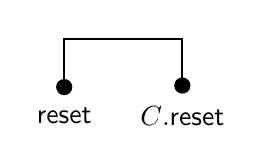
\begin{tikzpicture}[shorten >=1pt,node distance=.7cm,>=stealth']

      \node (start) {};
      \node(h4)[left of=start]{}; %, node distance=1.5cm

      \node[node distance=1cm] (ab) [below of=start] {\NameCtrl.\PortReset};
      \node[node distance=1.5cm] (aa) [left of=ab]{\PortReset};

      \draw [style=-*, thick, black]  ($(h4.south)+(0,.1cm)$) -| (ab.north);
      \draw [style=-*, thick, black]  ($(h4.south)+(0,.1cm)$) -| (aa.north);
    \end{tikzpicture}
%
    &
%
    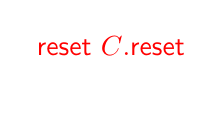
\begin{tikzpicture}[shorten >=1pt,node distance=.7cm,>=stealth']
      \node (start) {\color{red}\PortReset\ \NameCtrl.\PortReset};
      \node()[below of=start]{};
    \end{tikzpicture}
%
    &
%
    {\color{red}$
    \begin{aligned}[b]
      \NameCtrl.\PortReset &\Rightarrow \PortReset
      \\
      \PortReset &\Rightarrow \NameCtrl.\PortReset
      \\
      \true &\Rightarrow
      \PortReset \land \NameCtrl.\PortReset
    \end{aligned}
    $}
%
    \\\hline
  \end{tabular}}
\end{table}

\noteEM{Dans le paragraph precedent, tu resume le cas des connecteurs sans data, dans les prochains, tu formalise avec data, mais pour le lecteur ``casual'', le changement n'est pas evident... }
Below, we assume that, as in \fig{schema:ArchFailure:BIP}, the
interaction model is defined by a set of connectors, annotated with
Boolean guards and with update assignments.  In particular, we assume
that the guards and update assignments are well-defined for any
interaction allowed by the connector.  For example, the choice
$\NameCtrl.\PortFail\ ?\ \NameCtrl.\mathit{zone} : \topinterval$ in
the update assignement
$
\NameTimer.\mathit{z} := \NameTimer.\mathit{z}
\cap \bigl(
(
\NameCtrl.\PortFail\ ?\ \NameCtrl.\mathit{zone} : \topinterval
)
+ \NameTimer.\mathit{t} \bigr)
$
associated to the connector {\NameTimer.\PortTick \trigsynch
  (\PortFail \trigsynch \NameCtrl.\PortFail)} in
\fig{schema:ArchFailure:BIP} ensures that the assignment is
well-defined independently of whether {\NameCtrl.\PortFail}
participates or not.  Let us denote by $\gamma \subset \ac(P_A)
\times \guards{V_A} \times \assigns{V_A}$ the set of connectors in the
architecture $A$ and by $P_x$ the set of ports involved in the
connector $x \in \gamma$.  Then, \addSB{the interaction model defined by $\gamma$ is 
  $\Gamma = \setdef{(a,g,u)}{(x,g,u) \in \gamma, a \in \intsem{x}}$
  and the encoding of $\Gamma$ is} $\nopri[\Gamma] \bydef{=}
\setdef{\nopri[x,g,u]}{(x,g,u) \in \gamma}$, where $\nopri[x,g,u]$ is the synchronisation vector defined by
%
\begin{multline}
  \label{eq:nopri:connector}
  \nopri[x,g,u] \bydef{=}
  %% \Tuple{p\bigl(\export[A](p),{{\color{blue}\export[A]'(p),}}b_p\bigr)}^{p \in P_x}
  \Tuple{\Setdef{p\bigl(\export[A](p),\export[A]'(p),b_p\bigr)}{p \in P_x \cap P}}^{P \in P_C^{C \in \cC} \cup \partition}
  \rightarrow
  \alpha_p
  \\
  \left[
    \bigwedge R(\tau(x))\bigl[\nicefrac{b_p}{p}\bigr]
    \land
    \bigwedge_{(x := e_x) \in u} (?x' = e_x)
    \land
    \bigwedge_{x \in \export[A](x), x \not\in u} (?x' = x)
    \right]
  \,,
\end{multline}
%% \noteSB{Ought to group ports by components in
%%   $\Tuple{p\bigl(\export[A](p),\export[A]'(p),b_p\bigr)}^{p \in P_x}$...
%%   \newline
%%   Will probably restrict interactions to one port per component
%%   throughout the paper to simplify.
%% }
%
with $b_p$ a fresh Boolean variable, $\alpha_p$ a fresh name, $\tau :
\ac(P_A) \rightarrow \ct(P_A)$ and $R : \ct(P_A) \rightarrow
\cru(P_A)$ the two mappings defined in \app{transformations} and
illustrated in \tab{connectors}, $\bigl[\nicefrac{b_p}{p}\bigr]$ is
the substitution that replaces in the expression that preceeds it
all occurrences of $p$ by $b_p$.

\begin{theorem}
  The open automaton $\semopen{\nopri[A,\partition]}$ corresponding to
  $\nopri[A,\partition]$ is
  isomorphic to the LTS $\semopen{\Gamma\bigl(\cC_A, (B_D)^{D \in
      \partition}\bigr)}$ (see \defn{comp:semantics}), with, for each
  $D \in \partition$, the component $B_D \bydef{=} \tuple{\{q\}, q,
    V_D, \val{0}{D}, D, \export[D], \goesto{}}$, with
  a fresh state $q$ and
%
  \begin{align*}
    V_D &= \bigcup_{p \in D} \export[A](p)
    \,,
    &\val{0}{D}(v) &= \bot, \text{ for all $v \in V_D$}
    \,,\\
    \goesto{} &= \bsetdef{(q, p, \true, \noop, q)}{p \in D}
    \,,
    &\export[D](p) &= \export[A](p), \text{ for all $p \in D$}
    \,.
  \end{align*}
%
\end{theorem}
%
%% \begin{proof}[Sketch of a proof]
%%   \noteSB{This theorem is very probably correct: the key question is
%%   whether isomorphism is, indeed, the relation to use. In absence of
%%   silent transitions, must be the case.}
%%   The theorem follows from the correctness of $\tau$ and $R$ shown in
%%   \cite{BliSif10-causal-fmsd}.
%% \end{proof}


%% \todoSB{This repeats things that were already said before.  Will reduce.}
%% Observe now that this encoding can be optimised to remove unnecessary
%% Boolean variables and loop transitions marked by \false.  For
%% instance, consider the ports shown in red in the second column of
%% \tab{connectors}.  All these ports only appear in the roots of the
%% corresponding causal interaction trees and, furthermore, each of these
%% trees only has one root (see \app{trees}).  In such cases, as in the
%% {\NameTimer.\PortTick \trigsynch (\PortFail \trigsynch
%%   \NameCtrl.\PortFail)} example discussed above, the Boolean variables
%% and the \false-marked loop transitions associated to these ports can
%% be removed.  Furthermore, the rules associated to these ports in the
%% corresponding systems of causal rules (see the rules in red in the
%% third column of \tab{connectors}) become tautological and can also be
%% removed from the corresponding guards in \eq{nopri:connector}.

%% %****************************************************************
%% \subsection{Encoding with the maximal progress priority model}
%% \label{secn:enc:maxprog}

\bigskip
In order to encode the maximal progress priority model, one has to
introduce an additional Boolean variable, for each port, for which we
have introduced one in $\nopri[A, \partition]$.  Intuitively, the
variables introduced above determine whether the original transition
labeled by the port is executed (\true), or rather the corresponding
self-loop, introduced by the encoding (\false).  The new variables
determine whether \emph{there is an original transition labelled by
  $p$ that could be executed from the same state}, \ie[,] with $b_p$
the variable introduced above for the encoding without maximal
progress, $q \goesto{p(\true, b_p)} q'$ iff $\exists q'': q
\goesto{p(b_p)} q''$ with $b_p = \true$ in $\nopri[A, \partition]$.
Then, in the SV guard, we have to check whether \emph{all ports
  leading to $p$ in the causal tree $\tau(x)$ can be fired} (see
\app{transformations}).  If so, then $p$ must be fired, \ie
$p(\false)$ must be blocked.  %% This is pretty much straightforward, but
%% care must be taken when doing this in the general case, since causal
%% interaction trees can get pretty tricky due to $\oplus$ (see
%% \app{trees}).}
%****************************************************************
%****************************************************************

% \subsection{SMT encoding of open pNets}
% \label{secn:smt}



\section{Case study}
\label{secn:case-study}

%****************************************************************

%% \subsection{Verification of the characteristic properties}
%% Eric: je pense que ce soutitre est inutile...

\label{secn:arch:verif}

%% \begin{figure}[t]
%%   \centering
%%   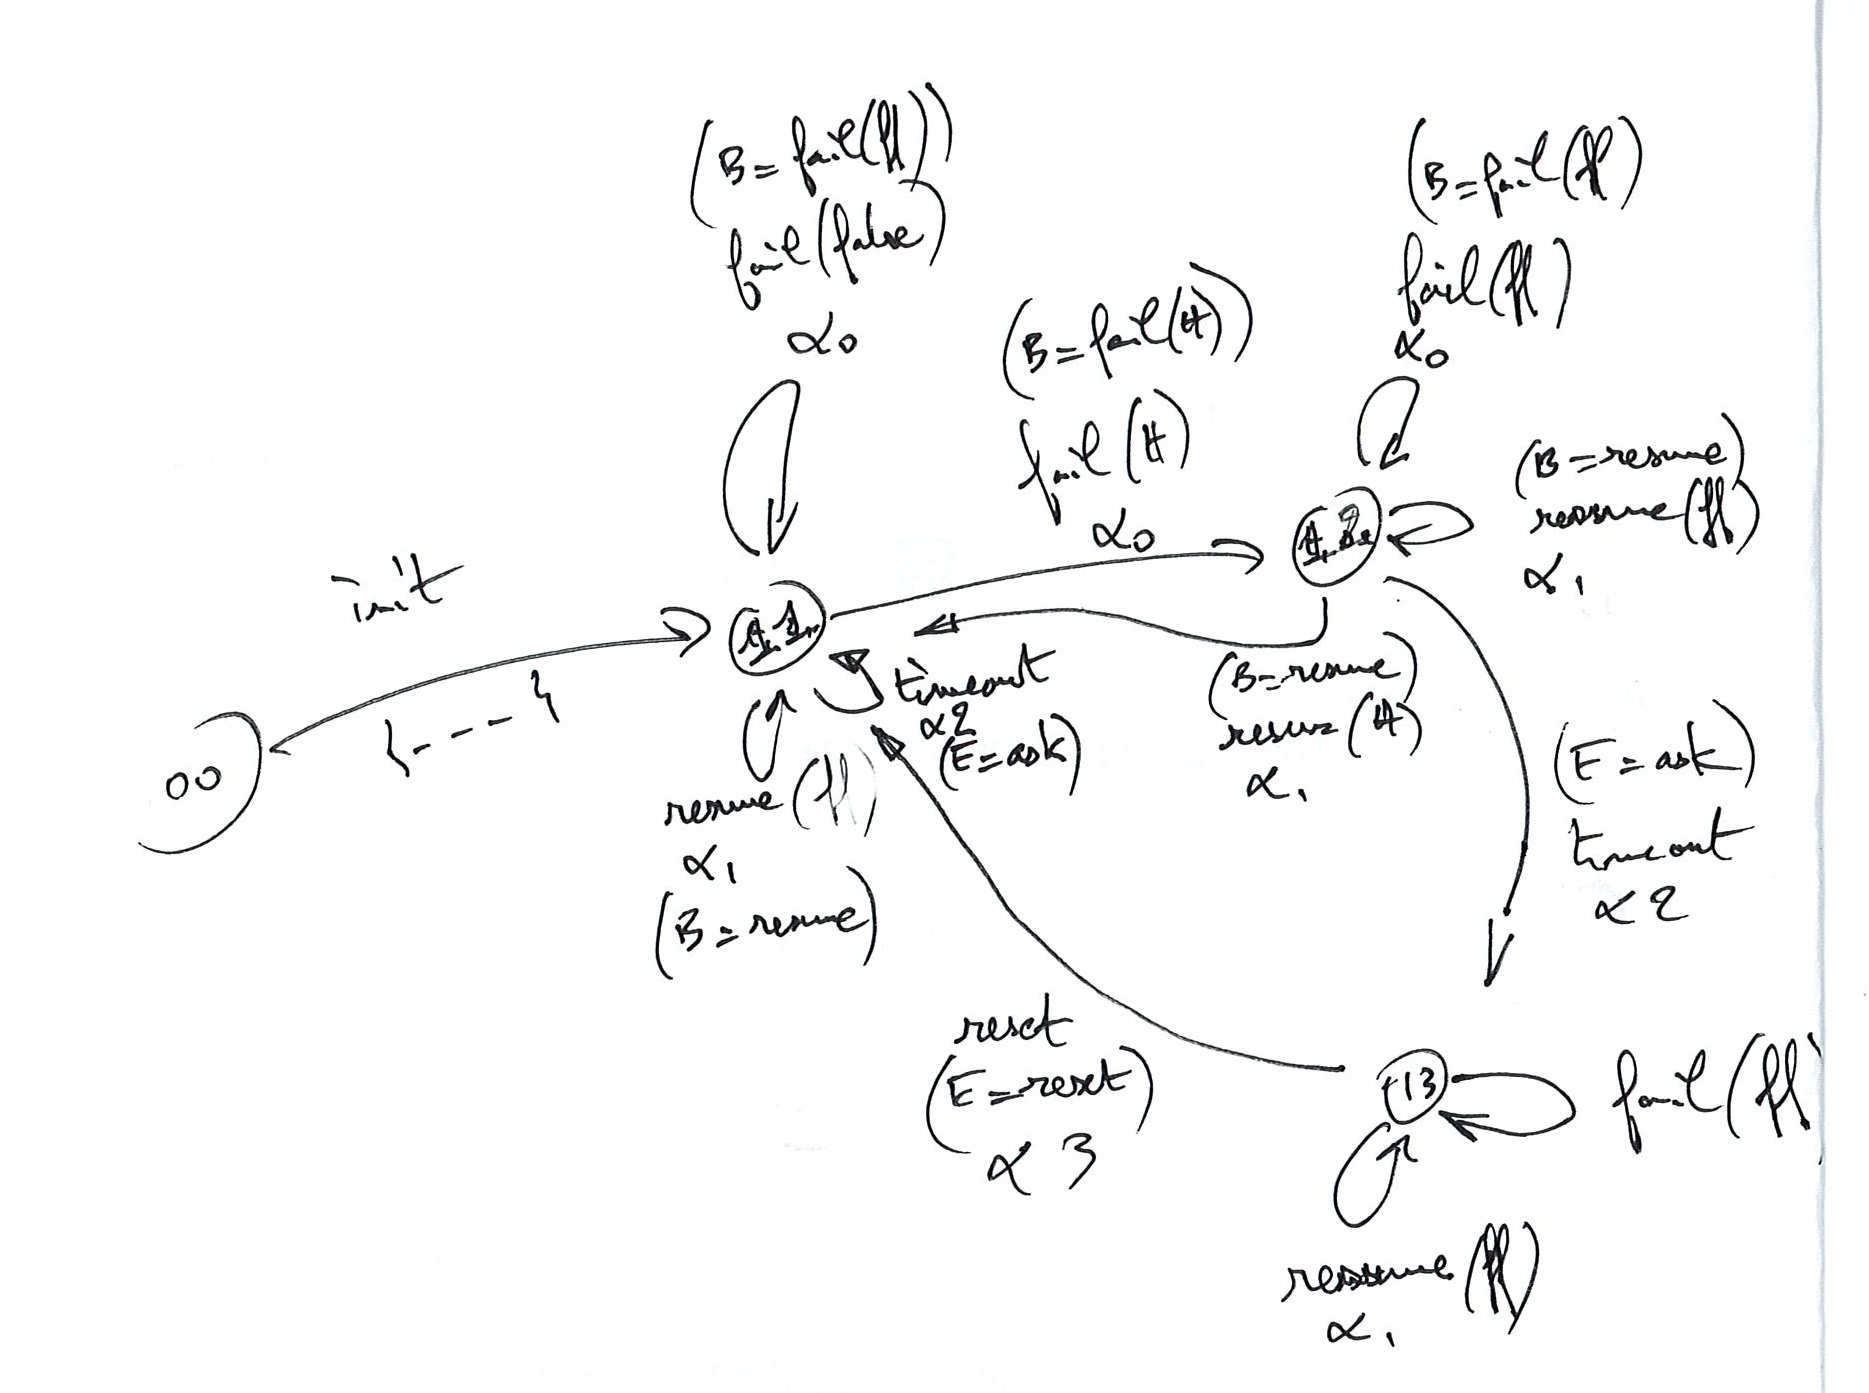
\includegraphics[width=\columnwidth]{TimerOpenAut}
%%   \caption{The open Automaton of the Failure Monitor Architecture}
%%   \label{schema:ArchFailure:BIP}
%% \end{figure}

\begin{figure}[t]
  \centering
  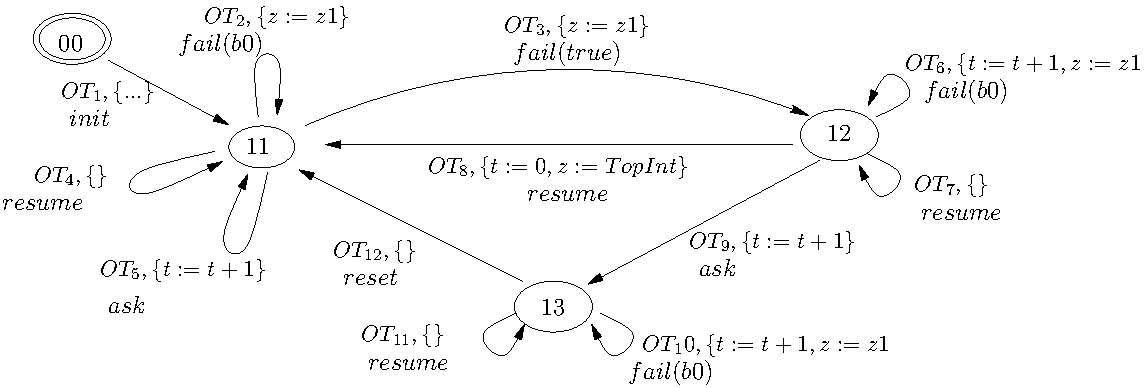
\includegraphics[width=0.9\columnwidth]{TimerOADetailed}
  \caption{The open Automaton of the Failure Monitor Architecture}
  \label{schema:ArchFailure:OA}
\end{figure}

In \cite{HMZ-FORTE2016QBMZ-AVOCS18}, we have described an algorithm
and a tool that 
computes the open automaton encoding the semantics of an open
pNet. This tool computes open transitions from the combinations of all
possible behaviours and synchronisation vectors of the pNet, then makes
use of an SMT engine to check satisfiability of the open transition
predicates, and minimize the size of the resulting automaton.

%% The encoding into the SMT language involves the definition of the
%% action and data domains and operators, and the axiomatisation of
%% domain-dependant properties, to allow the SMT engine to be as precise
%% as possible (even if it cannot be complete).

%% The resulting open automaton will later be subject to (symbolic)
%% model-checking and equivalence checking algorithms, themselves
%% requiring automatic proof assistance. \todoEM{trop flou pour le
%%   moment, mais je n'ose pas dire des trucs trop precis... meme si on a
%%   deja une implem de la FH-bisim, elle n'est pas validee!}

In Figure~\ref{schema:ArchFailure:OA} we show the full open automaton
obtained from our pNet. For reasons of space, we have not shown the
detail of the open transition, but only the assignments of state
variables, some usefull parts of the predicates, and the resulting
action; you can find the full details in 
Appendix \ref{secn:full-results}. As an example, $OT_3$ is the one
explained in Example~\ref{Example:TimerOT3} page~\pageref{Example:TimerOT3}

This automaton has 12 transitions, including those encoding various
possible firing of some interactions (e.g. OT 2 and 3 for
$fail$). At first sight, it appears the rough behaviour is
reasonable, although a detailed study shows that the property stated
in page~\pageref{property:reset} does not hold, because of the
$fail$ loops on states $11$ and $12$. This is because we did not use
the maximal progress assumption here. If we do, we get the corrected
behaviour in Fig~\ref{schema:ArchFailure:OA-MaxProgress}
(\app{full-results}), in which $OT_7$ has 
disappeared, and $OT_2$ and $OT_{10}$ have been restricted to
$b0=false$. This one verifies all the properties listed in
\app{properties}. 


%****************************************************************

\subsection{Composition of architectures}
\label{secn:arch:composition}

We now consider a system comprising two components $B_1$ and $B_2$
with the corresponding interfaces $\tuple{V_i, P_i,
  \export[i]}_{i=1,2}$, such that $\listset{\PortFail_i,
  \PortResume_i} \subseteq P_i$, for $i = 1,2$.

Assuming that the associated system requirements comprise the
capability of monitoring the failure events corresponding to ports
$\PortFail_1$ and $\PortFail_2$ of the two components, we would like
to apply two instances of the Failure Monitor architecture.  However,
we impose an additional constraint: only one timer coordinator is
allowed, for example because it must eventually be implemented by a
hardware component.

We consider two architecture instances $A_i = \tuple{\cC_i, V_{A_i},
  P_{A_i}, \export[A_i], \Gamma_i}$, for $i = 1,2$, with all their
constituting elements cloned from the Failure Monitor architecture of
the previous examples while substituting each entity $X$ by $X^i$.
For instance, the initialisation of the $\mathit{zone}$ variable is
transformed into $\IntervalInit[1]$ and $\IntervalInit[2]$,
respectively.  The only exception to this cloning procedure are the
sets of coordinating components: $\cC^i = \listset{\NameTimer,
  \NameCtrl^i}$, \ie the $\NameTimer$ component is shared, while
components $\NameCtrl^1$ and $\NameCtrl^2$ are obtained by making two
copies of $\NameCtrl$ as above.

In order to apply both architectures, we must verify that they are
upwards compatible and compute the combined interaction model $\Gamma$
in $A_1 \arcomp A_2 = \tuple{\cC_1 \cup \cC_2, V_{A_1} \cup V_{A_2},
  P_{A_1} \cup P_{A_2}, \export[A_1] \cup \export[A_2], \Gamma}$
(see \defn{arch:composition}).

\todoSBin{Complete this section}

%****************************************************************
%****************************************************************

\section{Related work}
\label{secn:related}
Previous works on pNets and BIP architectures have been mentioned at the beginning of the paper. Consequently, we  review here the closest related works outside the scope of pNets and BIP architectures. Among those, we focus on existing approaches for the compositional and parameterized verification of systems, and on alternative verification engines???
\noteLH{not sure about this classification ; to be refined}

%%A few tracks, pas r\'edig\'es...

%%% compositional verification
approaches by typing interfaces/protocols == Simon

%% infinite/parametrized model checking? == ERIC (listes ci-dessous)  + Simon

Basic research on behaviour models and verification algorithms for
data-sensitive systems started in the nineties, with the seminal work
of Hennesy, Lin, and their colleagues on value-passing systems with
assignments
\cite{CONCUR::Lin1996,HennessyL1995:353,APSEC::Lin2001}. Later, many
different works addressing various classes of infinite-state systems
and/or paramaterized topologies have been published, using
combinations of approaches, often including predicate abstraction and
SMT satisfiability (see
e.g. \cite{BruniEtAl-Tiles-Concur2000,DBLP:conf/cade/GhilardiNRZ08,DBLP:journals/jsat/AlbertiGPRR12,CimattiEtAl-NUXMV-CAV2014,ChampionEtAl-Kind2-CAV2016}). With
respect to these, we use symbolic representations not only to get a
finite representation of infinite spaces, but also to express the
(data-sensitive) synchronisations with the environment, making our
models suitable for compositional verification.

Among these works, several have shown the capacity of the SMT engines
(either Z3 or Yikes) as servers for solving verification conditions of
the algorithms, for large case-studies
(e.g. \cite{DBLP:journals/corr/CimattiGMT13,DBLP:journals/corr/abs-1806-11459}).
%% SMT on an application not using component structure. is there a strong Z3 example == Eric

As compositional proof of safety is difficult, some approaches rely on theorem proving to ensure the safety of component operations. Coqots and Pycots\cite{BCDLM:CBSE2014} even allow to prove the safety of reconfiguration procedures which are known to be highly difficult to verify, and massively parametrised. unfortunately the approach relies on a high expertise and significant efforts from the component user as (s)he must prove manually the safety of the reconfiguration process. In this paper, we rely on automatic encoding into a SMT solver making the proof of properties much more automatic, but we cannot prove the safety of the reconfiguration procedure.




In~\cite{DDJO:JLAMP2012}, the authors propose a compositional proof system for distributed objects that is suitable for implementation within the KeY framework~\cite{BHS:Key2007} and uses a Hoare logic approach.
The approach relies on history invariant for each object, separating local reasoning for proving object invariant from global reasoning that relies on well-formedness of traces. Compared to this  approach, we do not  deal with complex history-based specifications because we use interaction specification and SMT-reasoning instead of Hoare logic. Also the correctness of the composition is given by the properties of architectures which allows for more flexibility than well-formedness of traces.






%****************************************************************

%****************************************************************

\section{Conclusion}
\label{secn:conclusion}

What have we done.

Discussion:

- what did we lern about comparison of the coordination models ?

- extension to other priority features

- proof of correctness ?

%****************************************************************
%****************************************************************

\bibliographystyle{abbrv}
\bibliography{biblio,biblioFromPnets}

%****************************************************************
%****************************************************************
\appendix
\clearpage

%****************************************************************
%****************************************************************

\section{Proofs}
\label{secn:proofs}

\begin{lemma}
  \label{lem:onlyone}
  Let $A = \tuple{\cC, V_A, P_A, \export[A], \Gamma}$ be an architecture and denote
  by $\Gamma_\cC \bydef{=}
%
  \setdef{
    (a \cap P_\cC, \true, \noop)
  }{
    (a, g, e) \in \Gamma
  }$, with $P_\cC = \bigcup_{C \in \cC} P_C$,
%  
  the projection of $\Gamma$ onto the coordinating components of
  $A$.  Consider the architecture $A' = \tuple{\{C'\}, V_A, P_A, \export[A],
  \Gamma}$, where $C' = \Gamma_\cC(\cC)$.  For any set of
  components $\cB$, satisfying the conditions of
  \defn{arch:application}, we have
  $\semopen{A(\cB)} = \semopen{A'(\cB)}$.
\end{lemma}
%
\begin{proof}
  First of all, notice that, by \defn{im:sem},
  $V_{C'} = \bigcup_{C \in \cC} V_C$ and $P_{C'} = P_\cC = \bigcup_{C \in \cC} P_C$.
  The conditions of \defn{arch} are satisfied and $A'$ is indeed
  an architecture.  Furthermore, $\cB$ satisfies the conditions
  of \defn{arch:application} \wrt $A'$.  Hence, the component
  $A'(\cB)$ is well defined.

  Clearly the state spaces and initial states %% and interfaces
  of both LTSs $\semopen{A(\cB)}$ and $\semopen{A'(\cB)}$
  coincide.  Thus, we only have to prove that so do the
  transition relations.  Let us assume that
  $\cC = C_i^{i \in I}$ and $\cB = B_j^{j \in J}$.
  We will use $q_i, q_i'$ to denote the states of
  $C_i$ and $q_j, q_j'$ to denote the states of $B_j$,
  and similarly for the valuations of variables.

  By \defn{comp:semantics},
%
  \begin{equation}
    \label{eq:lem1:trans:sem}
    (q_i, \val{}{i})^{i \in I} (q_j, \val{}{j})^{j \in J}
    \goesto{a, \val[\tilde]{}{}}
    (q_i', \val{\prime}{i})^{i \in I}
    (q_j', \val{\prime}{j})^{j \in J}
  \end{equation}
%  
  is a transition in $\semopen{A(\cB)}$ (\resp
  $\semopen{A'(\cB)}$) iff
%
  \begin{equation}
    \label{eq:lem1:trans}
    q_i^{i \in I} q_j^{j \in J}
    \goesto{a, g', e'}
    (q_i')^{i \in I} (q_j')^{j \in J}
    \,,
  \end{equation}
%
  is a transition in $A(\cB)$ (\resp $A'(\cB)$) and
%
  \begin{mathpar}
    \val{i \in I}{i} \val{j \in J}{j}
    \models g'
    \,,
    \and
    (\val{\prime}{i})^{i \in I} (\val{\prime}{j})^{j \in J}
    = \val[\tilde]{}{}[e']
    \,,
    \and
    \valdiff{\val{i \in I}{i} \val{j \in J}{j}}{
      \val[\tilde]{}{}} \subseteq \export(a)       
  \end{mathpar}
%
  (with $\export$ defined as in \defn{arch:application}).

  By \defn{im:sem} and \defn{priority:sem}, \eq{lem1:trans} is a transition in $A(\cB)$
  iff $a \neq \emptyset$, $(a, g, e) \in \IMextend{\Gamma}{P}$,
  where $P = \bigcup_{B \in \cB \cup \cC} P_B$, and
  %
  \begin{enumerate}
  \item\label{ab:start} for $i \in I$,\\
    $a \cap P_{C_i} \neq \emptyset$ and
    $q_i \goesto{a \cap P_{C_i},\, g_{C_i},\, e_{C_i}} q_i'$
    is a transition in $C_i$, or\\
    $a \cap P_{C_i} = \emptyset$ and $q_i = q_i'$
    (for covenience, we put $g_{C_i} = \true$ and $e_{C_i} = \noop$ in item~\ref{aux1} below);
  \item for $j \in J$,\\
    $a \cap P_{B_j} \neq \emptyset$ and
    $q_j \goesto{a \cap P_{B_j},\, g_{B_j},\, e_{B_j}} q_j'$
    is a transition in $B_j$, or\\
    $a \cap P_{B_j} = \emptyset$ and $q_j = q_j'$
    (for covenience, we put $g_{B_j} = \true$ and $e_{B_j} = \noop$ in item~\ref{aux1} below);
  \item\label{ab:end}\label{aux1} $g' = g \land \bigwedge_{i \in I} g_{C_i} \land
    \bigwedge_{j \in J} g_{B_j} \land \varphi_\mu$ and
    $e' = e; e_{C_i}^{i \in I}, e_{B_j}^{j \in J}$, where    
%
    \begin{equation}
      \label{eq:only1:maxprog:guard}
      \varphi_\mu = \bigwedge_{
        \begin{array}{c}
          q_i^{i \in I} q_j^{j \in J} \goesto{b, h, f} \text{ in }
          (\IMextend{\Gamma}{P})(\cC \cup \cB)
          \\
          a \varsubsetneq b
        \end{array}
      } \lnot h
      \,.
    \end{equation}
%
  \breakenumistart

  Similarly, \eq{lem1:trans} is a transition in
  $A'(\cB)$ iff $a \neq \emptyset$,
  $(a, g, e) \in \IMextend{\Gamma}{P}$ and
%
  \breakenumiend
% 
  \item \label{a1b:start} \label{only1:coord}
    $a \cap P_{C'} \neq \emptyset$ and 
    $(q_i)^{i \in I} \goesto{a \cap P_{C'}, g_{C'}, e_{C'}} (q_i')^{i \in I}$
    is a transition in $C'$, or\\
    $a \cap P_{C'} = \emptyset$ and $q_i = q_i'$,
    for all $i \in [1,m]$
    (for covenience, we put $g_{C'} = \true$ and $e_{C'} = \noop$ in
    item~\ref{aux2} below);
  \item for $j \in J$,\\
    $a \cap P_{B_j} \neq \emptyset$ and
    $q_j \goesto{a \cap P_{B_j}, g_{B_j}, e_{B_j}} q_j'$
    is a transition in $B_j$, or\\
    $a \cap P_{B_j} = \emptyset$ and $q_j = q_j'$
    (for covenience, we put $g_{B_j} = \true$ and $e_{B_j} = \noop$ in
    item~\ref{aux2} below);
  \item\label{aux2} $g' = g \land g_{C'} \land
    \bigwedge_{j \in J} g_{B_j} \land \varphi_\mu'$ and
    $e' = e; e_{C'}, e_{B_j}^{j \in J}$ (with $\varphi_\mu'$ defined as
    in \eq{only1:maxprog:guard}, but substituting $\{C'\}$ instead of $\cC$).
%
  \breakenumistart
  Notice that, for any $i \in I$, since
  $P_{C_i} \subseteq P_{C'}$, we have
  $a \cap P_{C_i} = (a \cap P_{C'}) \cap P_{C_i}$.
  Thus, if $a \cap P_{C'} \neq \emptyset$, 
  the transition in condition~\ref{only1:coord} above is
  present in $C'$ iff
  $(a \cap P_{C'}, \true, \noop) \in \Gamma_\cC$ and
  \breakenumiend
% 
  \item for $i \in I$,\\
    $a \cap P_{C_i} \neq \emptyset$ and
    $q_i \goesto{a \cap P_{C_i}, g_{C_i}, e_{C_i}} q_i'$
    is a transition in $C_i$, or\\
    $a \cap P_{C_i} = \emptyset$ and $q_i = q_i'$,
    (for covenience, we put $g_{C_i} = \true$ and $e_{C_i} = \noop$ in
    item~\ref{aux3} below);
  \item \label{a1b:end} \label{aux3} $g_{C'} = \bigwedge_{i \in I} g_{C_i}$ and
    $e_{C'} = e_{C_i}^{i \in I}$.
  \end{enumerate}

  Consider $(a,g,e) \in \IMextend{\Gamma}{P}$.  By
  \defn{arch:application}, this is equivalent to
  $(a \cap P_A, g, e) \in \Gamma$.
  Since $P_{C'} = P_\cC \subseteq P_A$, we have
  $a \cap P_{C'} = a \cap P_\cC = (a \cap P_A) \cap P_\cC$.
  Hence, by the definition of $\Gamma_\cC$ in the lemma statement,
  this is also equivalent to
  $(a \cap P_{C'}, \true, \noop) \in \Gamma_\cC$.

  Thus, conditions \ref{ab:start}\ndash\ref{ab:end} are satisfied iff
  so are conditions \ref{a1b:start}\ndash\ref{a1b:end} (to see that
  $\varphi_\mu$ is satisfied iff so is $\varphi_\mu'$, one has to
  consider the same two sets of conditions, but this time without the
  additional conjuncts $\varphi_\mu$ and $\varphi_\mu'$ in
  items~\ref{aux1} and \ref{aux2}, since no priority model is applied
  to obtain $C'$).  This proves that the transition relations of
  $\semopen{A(\cB)}$ and $\semopen{A'(\cB)}$ coincide and, therefore,
  $\semopen{A(\cB)} = \semopen{A'(\cB)}$.
\end{proof}

\begin{note}
  \label{rem:upwards:compat}
  Notice that, since, in the statement of \lem{onlyone}, 
  %
  \begin{enumerate}
  \item the interaction models are the same for both $A$ and $A'$, and
  \item $P_{C'} = P_\cC$,
  \end{enumerate}
  %
  substituting $A'$ for $A$ preserves upwards compatibility, \ie for any
  architecture $A''$, holds the following statement: $A$ and $A''$ are
  upwards compatible if and only if so are $A'$ and $A''$.
\end{note}

\begin{lemma}
  \label{lem:onestep}
  Let $\cB$ be a set of components; let $A_i = \tuple{\{C_i\}, V_{A_i},
  P_{A_i}, \export[A_i], \Gamma_i}$, for $i = 1,2$, be two upwards compatible architectures
  with one coordinator each, applicable to $\cB$.  Denote
  $P_i = P_{C_i} \cup \bigcup_{B \in \cB} P_B$.
  Finally, let
%
  $
  s_1 s_2 s
%
  \goesto{a, \tilde{\val{}{}}}
%
  s_1' s_2' s'
  $,
%
  be a transition in $\semopen{(A_1 \arcomp A_2)(\cB)}$, with
  $a \neq \emptyset$, 
  $s, s' \in \prod_{B \in \cB} S_{\semopen{B}}$
  and
  $s_i, s_i' \in S_{\semopen{C_i}}$ ($i=1,2$).
%
  Then, for $i=1,2$, either $a \cap P_i = \emptyset$ and $s_i s=
  s_i' s'$, or there exists a transition
%
  $
  s_i s
%
  \goesto{a \cap P_i, \val[\doubletilde]{}{}}
%
  s_i' s''
  $ 
%
  in $\semopen{A_i(\cB)}$, with
  $\val[\doubletilde]{}{}$ being the restriction of
  $\val[\tilde]{}{}$ to
  $V_i = V_{C_i} \cup \bigcup_{B \in \cB} V_B$ and
  $s' \order s''$.
\end{lemma}
%
\begin{proof}
  By \defn{comp:semantics}, every semantic state consists of a
  component state and a valuation of component variables.  Thus,
  we can expand $s_1 s_2 s \goesto{a, \tilde{\val{}{}}} s_1' s_2' s'$
  as
%
  \[
  (q_1, \val{}{1}, q_2, \val{}{2}, q, \val{}{})
%
  \goesto{a, \tilde{\val{}{}}}
%
  (q_1', \val[\primeit]{}{1}, q_2', \val[\primeit]{}{1}, q', \val[\primeit]{}{})
  \,.
  \]
%
  By \defn{im:sem} and \defn{priority:sem}, this implies
  that
  $(q_1, q_2, q) \goesto {a, g', e'} (q_1', q_2', q')$
  is a transition in $(A_1 \arcomp A_2)(\cB)$, with
%
  $g' = g \land g_1 \land g_2 \land g_\cB \land \varphi_\mu$
  and
  $e' = e; (e_1, e_2, e_\cB)$,
  where $(a, g, e) \in \Gamma$ (see \eq{arch:composition} for the
  definition of $\Gamma$);
%  
  $g_1$, $g_2$ and $e_1$, $e_2$ are, respectively, the guards and
  update expressions of the underlying transitions in the coordinating
  components $C_1$ and $C_2$;
%    
  \begin{mathpar}
    g_\cB = \bigwedge_{B \in \supp{a} \cap \cB} g_B
    \,,
    \and
    e_\cB = e_B^{B \in \supp{a} \cap \cB}
    \,,
  \end{mathpar}
%
  are the compositions of, respectively, the guards and update
  expressions of the operand components;
%    
  \begin{equation}
    \label{eq:onestep:maxprog:guard}
    \varphi_\mu = \bigwedge_{
      \begin{array}{c}
        (q_1, q_2, q) \goesto{b, h', f'} \text{ in }
        \bigl(\IMextend{\Gamma}{(P_1 \cup P_2)}\bigr)
        \bigl(\{C_1, C_2\} \cup \cB\bigr)
        \\
        a \varsubsetneq b
      \end{array}
    } \lnot h'
  \end{equation}
%
  is the conjunct encoding the maximal progress priority in
  \defn{priority:sem}.  As above for $g'$, for each $(b, h', f')$ in
  \eq{onestep:maxprog:guard}, $h'$ can be decomposed as $h' = h \land
  h_1 \land h_2 \land h_\cB$ (without the maximal progress conjunct,
  since no priority is applied in $\bigl(\IMextend{\Gamma}{(P_1 \cup
    P_2)}\bigr)\bigl(\{C_1, C_2\} \cup \cB\bigr)$).
  
  By \eq{comp:semantics}, we also have
%
  \begin{align}
    \label{eq:guard}
    (\val{}{1}, \val{}{2}, \val{}{}) &\models g'
    \,,
    \\
    \label{eq:substitution}
    (\val[\primeit]{}{1}, \val[\primeit]{}{2}, \val[\primeit]{}{})
    &= \val[\tilde]{}{}[e']
    \,,
    \\
    \label{eq:transient}
    \valdiff{(\val{}{1}, \val{}{2}, \val{}{})}{\val[\tilde]{}{}}
    &\subseteq \export(a)
    \,.
  \end{align}
%
  If $a \cap P_1 = \emptyset$, then $\supp{a} = \{C_2\}$ and, by
  \eq{transient} and \defn{im:sem}, $s_1 = s_1'$ and $s = s'$
  (recall, \defn{im}, that, for $(a,g,e) \in \Gamma$, we have $e
  \in \exprs{V_a}$).  Hereafter, assume $a \cap P_1 \neq
  \emptyset$.

  By \eq{arch:composition}, for $i=1,2$, there exist $(a \cap P_{A_i},
  g^i, e^i) \in \Gamma_i$, such that $g = g^1 \land g^2$ and $e = e^1
  \land e^2$.
  %% Similarly, for each $(b, h', f')$ in \eq{onestep:maxprog:guard},
  %% there exist $(b \cap P_{A_i}, h^i, f^i) \in \Gamma_i$, such that
  %% $h = h^1 \land h^2$ and $f = f^1 \land f^2$.
%
  We want to show that the interaction $(a \cap P_1, g^1, e^1)$ is
  enabled in the state $(q_1, \val{}{1}, q, \val{}{})$ of
  $\semopen{A_1(\cB)}$.  To this end, we proceed in two steps:
%
  \begin{enumerate}
  \item \label{onestep:proof:im} We show that $(a \cap P_1, g^1,
    e^1)$ is enabled in the state $(q_1, \val{}{i}, q, \val{}{})$ of
    $\semopen{(\IMextend{\Gamma_1}{P_1})(\cB)}$.
  \item \label{onestep:proof:maxp} We show that $(a \cap P_1, g^1,
    e^1)$ is not inhibited in $\semopen{A_1(\cB)} =
    \semopen{\mu\bigl((\IMextend{\Gamma_1}{P_1})(\cB)\bigr)}$ by the
    maximal progress priority.
  \end{enumerate}

  \paragraph*{Step \ref{onestep:proof:im}}
  %% Denoting $P_\cB = \bigcup_{B \in \supp{a} \cap \cB} P_B$, 
  By \defn{im:sem}, we have
%
  \begin{mathpar}
    q_1 \goesto{a \cap P_{C_1}, g_1, e_1} q_1'
    \and
    \text{and}
    \and
    q_B \goesto{a \cap P_B, g_B, e_B} q_B',
    \text{ for each }
    B \in \cB
    \,.
  \end{mathpar}

  By \eq{guard}, we have
  $(\val{}{1}, \val{}{}) \models g^1 \land g_1 \land g_\cB$.

  Denoting \todoSB{One tilde is enough}$\val[\doubletilde]{}{1}$ the restriction of
%
  $\val[\tilde]{}{}$ to
  $V_1 = V_{C_1} \cup \bigcup_{B \in \cB} V_B$,
%
  we have, by \eq{substitution} and the monotonicity of
  expressions,
%
  $(\val[\primeit]{}{1}, \val[\primeit]{}{}) \order
  \val[\doubletilde]{}{1}[e^1; (e_1, e_b)]$.  \todoSB{Remove this}\hl{Notice that all
  variables affected by both $e^1$ and $e^2$ must necessarily
  belong to $\bigcup_{B \in \cB} V_B$.}  Hence,
%
  $\val[\doubletilde]{}{1}[e^1; (e_1, e_b)] =
  (\val[\primeit]{}{1}, \val[\secondit]{}{})$ with 
  $\val[\primeit]{}{} \order \val[\secondit]{}{}$.

  By \defn{comp:semantics} and \defn{im:sem}, we have
  $
  (q_1, \val{}{1}, q, \val{}{})
  \goesto{a \cap P_1, \val[\doubletilde]{}{1}}
  (q_1', \val[\primeit]{}{1}, q, \val[\secondit]{}{})
  $ in $\semopen{(\IMextend{\Gamma_1}{P_1})(\cB)}$.

  Symmetrically, we have 
  $
  (q_2, \val{}{2}, q, \val{}{})
  \goesto{a \cap P_2, \val[\doubletilde]{}{2}}
  (q_2', \val[\primeit]{}{2}, q, \val[\secondit]{}{})
  $ in $\semopen{(\IMextend{\Gamma_2}{P_2})(\cB)}$.   
   
  \paragraph*{Step \ref{onestep:proof:maxp}}
  Suppose that $a \cap P_1 \varsubsetneq b_1$, for some interaction
  $(b_1, h^1, f^1) \in \IMextend{\Gamma_1}{P_1}$ enabled in $(q_1,
  \val{}{1}, q, \val{}{})$.  Then, by upwards compatibility of $A_1$
  and $A_2$, there exists $(b_2, h^2, f^2) \in
  \IMextend{\Gamma_2}{P_2}$, enabled in $(q_2, \val{}{2}, q,
  \val{}{})$, such that $a \cap P_2 \subseteq b_2$ and $b_2 \cap P_1 =
  b_1 \cap P_2$.  By \defn{arch:application}, we have $(b_1 \cap P_{A_1},
  h^1, e^1) \in \Gamma^1$.  Furthermore,
%
  \begin{multline*}
    ((b_1 \cap P_{A_1}) \cup (b_2 \cap P_{A_2}))  \cap P_{A_1} =
    (b_1 \cap P_{A_1}) \cup (b_2 \cap P_{A_1} \cap P_{A_2}) =\\
    (b_1 \cap P_{A_1}) \cup ((b_2 \cap P_1) \cap P_{A_1} \cap P_{A_2}) =  
    (b_1 \cap P_{A_1}) \cup ((b_1 \cap P_2) \cap P_{A_1} \cap P_{A_2}) =\\
    (b_1 \cup (b_1 \cap P_2 \cap P_{A_2})) \cap P_{A_1} =
    b_1 \cap P_{A_1} 
  \end{multline*}
%
  Symmetrically, $(b_2 \cap P_{A_2}, h^2, e^2) \in \Gamma^2$ and
  $((b_1 \cap P_{A_1}) \cup (b_2 \cap P_{A_2})) \cap P_{A_2} = b_2
  \cap P_{A_2}$.  By \eq{arch:composition}, we then have $((b_1 \cap
  P_{A_1}) \cup (b_2 \cap P_{A_2}), h^1 \land h^2, f^1 \expmix f^2)
  \in \Gamma$ and, by \defn{arch:application}, $(b_1 \cup b_2, h^1 \land
  h^2, f^1 \expmix f^2) \in \IMextend{\Gamma}{(P_1 \cup P_2)}$.
%
  Since both $(b_i, h^i, f^i) \in \IMextend{\Gamma_i}{P_i}$ are
  enabled in the respective states $(q_i, \val{}{i}, q, \val{}{})$, we
  conclude that $(b_1 \cup b_2, h^1 \land h^2, f^1 \expmix f^2)$ is
  enabled in $(q_1, \val{}{1}, q_2, \val{}{2}, q, \val{}{})$.

  Since $a \cap P_1 \varsubsetneq b_1$ and $a \cap P_2 \subseteq b_2$,
  we have $a \varsubsetneq b_1 \cup b_2$.  Thus, $(b_1 \cup b_2, h^1
  \land h^2, f^1 \expmix f^2)$ contribute to $\varphi_\mu$ in
  \eq{onestep:maxprog:guard}.  Since $(b_1 \cup b_2, h^1 \land h^2,
  f^1 \expmix f^2)$ is enabled in $(q_1, \val{}{1}, q_2, \val{}{2}, q,
  \val{}{})$, we have $(\val{}{1}, \val{}{2}, \val{}{}) \models h^1
  \land h^2$ and, therefore $(\val{}{1}, \val{}{2}, \val{}{})
  \not\models \varphi_\mu$, which contradicts \eq{guard}, thereby
  proving that $(a \cap P_1, g^1, e^1)$ is not inhibited in
  $\semopen{A_1(\cB)} =
  \semopen{\mu\bigl((\IMextend{\Gamma_1}{P_1})(\cB)\bigr)}$ by the
  maximal progress priority.

  The corresponding statement for $(a \cap P_2, g^2, e^2)$ is obtained
  symmetrically.
\end{proof}

\begin{lemma}
  \label{lem:stepabove}
  Consider a component $B$ and let 
%
  $
  (q_1, \val{}{1})
%
  \goesto{a, \val[\tilde]{}{}}
%
  (q_2, \val{}{2})
  $,
%
  be a transition in $\semopen{B}$.  For any valuation
  $\val[\primeit]{}{1}$, such that
  $\val{}{1} \order \val[\primeit]{}{1}$ and
  $\valdiff{\val{}{1}}{\val[\primeit]{}{1}} \subseteq \export(a)$,
  there exists a transition
%
  $
  (q_1, \val[\primeit]{}{1})
%
  \goesto{a, \val[\tilde]{}{}}
%
  (q_2, \val{}{2})
  $
%
  in $\semopen{B}$.
\end{lemma}
%
\begin{proof}
  By \eq{comp:semantics}, we have
%
  \begin{mathpar}
    q_1 \goesto{a, g, e} q_2
    \,,
    \and
    \val{}{1} \models g
    \,,
    \and
    \val{}{2} = \val[\tilde]{}{}[e]
    \,,
    \and
    \text{and}
    \and
    \valdiff{\val{}{1}}{\val[\tilde]{}{}} \subseteq \export(a)
    \,.
  \end{mathpar}

  By monotonicity of guards, we deduce
  $\val[\primeit]{}{1} \models g$.
  For any $v \not\in \export(a)$,
  $\val[\primeit]{}{1}(v) = \val{}{1}(v) = \val[\tilde]{}{}(v)$.
  Hence, 
  $\valdiff{\val[\primeit]{}{1}}{\val[\tilde]{}{}}
  \subseteq \export(a)$.
  By \eq{comp:semantics}, we conclude 
%
  $
  (q_1, \val[\primeit]{}{1})
%
  \goesto{a, \val[\tilde]{}{}}
%
  (q_2, \val{}{2})
  $.  
\end{proof}

\begin{proof}[Proof of \thm{combining}]
  By \lem{onlyone}, we can assume without loss of generality that each of the two
  architectures has only one coordinating component.  For $i =
  1,2$, we denote $\{C_i\} = \cC_i$, $P_i = P_{C_i}
  \cup\ \bigcup_{B \in \cB} P_B$ and $V_i = V_{C_i}
  \cup\ \bigcup_{B \in \cB} V_B$.
%
  By \rem{upwards:compat}, this does not affect their upwards
  compatibility, hence neither does this affect the applicability of
  \lem{onestep} below.
  
  The initiality of $\Phi_1 \land \Phi_2$, is trivial: both
  $\Phi_1$ and $\Phi_2$ are initial, hence $s^0 \models \Phi_1
  \land \Phi_2$.

  Consider a path
%
  \[
  s^0_1 s^0_2 s^0
%
  \goesto{a^1, \val[\tilde]{1}{}}
%
  s^1_1 s^1_2 s^1
%
  \goesto{a^2, \val[\tilde]{2}{}}
  \cdots
  \goesto{a^k, \val[\tilde]{k}{}}
%
  s^k_1 s^k_2 s^k
  \]
%
  in $\semopen{(A_1 \arcomp A_2)(\cB)}$, where
  $s^0,\dots,s^k \in \prod_{B \in \cB} S_{\semopen{B}}$ and
  $s^0_i,\dots, s^k_i \in S_{\semopen{C_i}}$, for $i=1,2$.
  We have to show that $s^k \models \Phi_1 \land \Phi_2$.

  Assuming that $a^1 \cap P_1 \neq \emptyset$, by \lem{onestep},
  there exists $s^{1\prime} \in \prod_{B \in \cB} S_{\semopen{B}}$,
  such that
%
  \[
  s^0_1 s^0
%
  \goesto{a^1 \cap P_1, \val[\doubletilde]{1}{}}
%
  s^1_1 s^{1\prime}
  \]
%
  is a transition in $\semopen{A_1(\cB)}$ with
  $\val[\doubletilde]{1}{}$ being the restriction of
  $\val[\tilde]{1}{}$ to $V_1$ and
  $s^1 \order s^{1\prime}$.
%
  By \lem{stepabove}, 
  \[
  s^1_1 s^1_2 s^{1\prime}
%
  \goesto{a^2, \val[\tilde]{2}{}}
%
  s^2_1 s^2_2 s^2
  \]
  is a transition in $\semopen{(A_1 \arcomp A_2)(\cB)}$ and,
  therefore, 
  \[
  s^1_1 s^1_2 s^{1\prime}
%
  \goesto{a^2, \val[\tilde]{2}{}}
%
  s^2_1 s^2_2 s^2
%
  \goesto{a^3, \val[\tilde]{3}{}}
  \cdots
  \goesto{a^k, \val[\tilde]{k}{}}
%
  s^k_1 s^k_2 s^k
  \]
%  
  is a path in $\semopen{(A_1 \arcomp A_2)(\cB)}$.
%
  Notice that, if the above assumption, $a^1 \cap P_1 \neq
  \emptyset$, does not hold, then $s^0_1 = s^1_1$, $s^0 = s^1$
  and we can take $s^{1\prime} = s^1$ in this latter path.

  Repeating the entire argument $k-1$ times, starting with this
  shorter path, we obtain a path
%
  \begin{equation}
    \label{eq:path-in-1}
    s^0_1 s^0
    %
    \goesto{a^1 \cap P_1, \val[\doubletilde]{1}{}}
    %
    s^1_1 s^{1\prime}
    %
    \goesto{a^2 \cap P_1, \val[\doubletilde]{2}{}}
    %
    s^2_1 s^{2\prime}
    %
    \goesto{a^3 \cap P_1, \val[\doubletilde]{3}{}}
    \cdots
    \goesto{a^k \cap P_1, \val[\doubletilde]{k}{}}
    %
    s^k_1 s^{k\prime}
  \end{equation}
%  
  with $s^i \order s^{i\prime}$, for all $i \in [1,k]$.

  From \eq{path-in-1}, we conclude that the state $s^k_1
  s^{k\prime}$ is reachable in $\semopen{A_1(\cB)}$.  Since $A_1$
  enforces $\Phi_1$ on $\cB$, this implies that $s^{k\prime}
  \models \Phi_1$.  Since $s^k \order s^{k\prime}$, we deduce, by
  \defn{property}, that $s^k \models \Phi_1$.

  Symmetrically, $s^k \models \Phi_2$, which concludes
  the proof.
\end{proof}

%*********************************************************************
%*********************************************************************
%
%\section{pNets additional definitions}
%\label{secn:pNets:additional}
%
%\begin{definition}[Sorts, Holes, Leaves of pNets]
%  \begin{itemize}
%  \item  \noteSB{I think this can be lightened up a bit, since the definitions are all 
%  straightforward, whereas the notation is complex.  Maybe reformulate in words and move 
%  the formal definitions in the appendix?}
% The sort of a pNet is its signature, i.e. the set of actions it can
%perform. \noteSB{Is there any chance that, by writing assignments explicitly ($x := e$), 
%we could eliminate the need to distinguish the input variables at all? That would 
%simplify things.}\hl{In the definition of sorts, we do not need to distinguish
%input variables} (that specify the dataflow within LTSs), so for
%computing LTS sorts, we use a substitution operator\footnote{$\subst{y_k\gets x_k}^{k\in 
%K}$ is the parallel substitution 
%operation.} to remove the
%\emph{input marker} of variables\footnote{$\overline{S}$ denotes a set of $S$.}. Formally:
%\[
%\begin{array}{l}
%\Sortop(\mylangle S,s_0, \to\myrangle) = \{\alpha\subst{x \gets ?x| 
%x\in\symb{iv}(\alpha)}|s \xrightarrow{\langle \alpha,~g,~(x_j\!:= {e}_j)^{j\in
%    J}\rangle} s'\in \to \} \\
%\Sortop(\mylangle \overline{\pNet}\!, %\pNet_i^{i\in I}, \Sort_j^{j\in J}
%\overline{\pNet}\!,
%\overline{\symb{SV}}\myrangle)
%=\{\alpha' |\, \overline{\alpha}%\alpha_j^{j\in J_k}
%\to\alpha'\in\set{\symb{SV}}\}
%\end{array}
%\]
%
%\item
%The set of holes of a pNet is defined inductively; the sets of holes
%in a pNet node and its subnets are all disjoint:
%  \[\begin{array}{l}
%\Holes(\mylangle S,s_0, \to\myrangle) \!=\! \emptyset \\
%\Holes(\mylangle \pNet_i^{i\in I}\!,\Sort_j^{j\in J}\!, \overline{\symb{SV}}\myrangle) 
%=J\uplus{\displaystyle \bigcup_{i\in 
%I}\Holes(\pNet_i)}\\
%\forall i\in I.\, \Holes(\pNet_i)\cap J=\emptyset\\
%\forall i_1,i_2\in I.\,i_1\neq i_2\Rightarrow  
%\Holes(\pNet_{i_1})\cap\Holes(\pNet_{i_2})=\emptyset
%\end{array}\]
%\item
%The set of leaves of a pNet is the set of all pLTSs occurring in the structure, defined 
%inductively as:
%\[\begin{array}{l}
%\Leaves(\mylangle S,s_0, \to\myrangle) \!=\!\emptyset\\%\{\mylangle S,s_0, \to\myrangle\}\\
%\Leaves(\mylangle \pNet_i^{i\in I}\!,%Sort_j^{j\in J}
%\overline{\Sort}\!, \overline{\symb{SV}}\myrangle) = {\displaystyle \biguplus_{i\in 
%I}\Leaves(\pNet_i)\uplus\{i\mapsto \pNet_i|\pNet_i\pNet_i \text{ is a }\pLTS\}}
%\end{array}\]
%\end{itemize}
%\end{definition}

%*********************************************************************
%*********************************************************************

\section{Algebraic representations of the interaction model}
\label{secn:algebras}

In this section condensed from
\cite[Section~4]{BarBliu15-offer-scico}, we briefly recall the syntax
and semantics of the algebras used to represent BIP interaction models
\emph{disregarding variables and data transfer}.  All the algebras are
parameterised by a set $P$ of all the ports in a given system.  The
semantics of the Algebra of Interactions $\ai(P)$ is given in terms of
sets of interactions by a function $\intsem{\cdot}: \ai(P) \rightarrow
2^{2^P}$.  The corresponding equivalence relation on $\ai(P)$ is
defined as follows: two terms $x,y \in \ai(P)$ are {\em equivalent} $x
\simeq y$ iff $\intsem{x} = \intsem{y}$.  For any other algebra
$\cA(P)$ among those appearing in this section, we define its
semantics by the function $\aisem{\cdot}: \cA(P) \rightarrow \ai(P)$.
A function $\intsem{\cdot}: \cA(P) \rightarrow 2^{2^P}$ is obtained by
composing $\aisem{\cdot}: \cA(P) \rightarrow \ai(P)$ and
$\intsem{\cdot}: \ai(P) \rightarrow 2^{2^P}$.  The axiomatisation of
$\ai(P)$ given in \cite{BliSif07-acp-emsoft} is sound and complete
with respect to $\simeq$.  Hence, for other algebras, the equivalences
induced by $\intsem{\cdot}$ and $\aisem{\cdot}$ coincide.

Below, we assume that a set of ports $P$ is given, such that $0,1\not\in
P$.

For any set $X$ of propositional variables, we denote by $\sB[X]$ the
corresponding Boolean algebra generated by $X$.  For presentation
clarity, we will often omit the conjunction operator and write $a \lor
bc$ instead of $a \lor (b \land c)$.


% *********************************************************************

\subsection{Algebra of Interactions}
\label{secn:ai}

The Algebra of Interactions is used to define the interaction semantics of other algebras. The elements of this algebra can be bijectively mapped to interaction models, \ie subsets of $2^P$.

\begin{syntax}
The syntax of the {\em Algebra of Interactions}, $\ai(P)$, is defined by
the following grammar
%
\begin{equation} \label{eq:apsynt}
  \begin{array}{rc*{4}{l@{\ |\ }}l}
    x & ::= & 0 & 1 & p \in P & x\cdot x & x + x \,,\\
  \end{array}
\end{equation}
%
where `$+$' and `$\cdot$' are binary operators, respectively called
{\em union} and {\em synchronisation}.  Synchronisation binds stronger
than union.
\end{syntax}
%
As follows from the interaction semantics given below, the additive
identity element $0$ represents blocking, since it does not authorise
any interaction.  The multiplicative identity element $1$ corresponds
to the empty interaction, which represents idling (see the discussion
in \cite{BarBliu15-offer-scico}).

\begin{semantics}
The semantics of $\ai(P)$ is given by the function $\|\cdot\| : \ai(P)
\rightarrow 2^{2^P}$, defined by
%
\begin{equation} \label{eq:apsem}
  \renewcommand{\arraystretch}{1.5}
  \begin{array}{lcl}
    \lefteqn{\|0\|\ =\ \emptyset,\quad \|1\|\ =\ \{\emptyset\},\quad
      \|p\|\ =\ \Big\{\{p\}\Big\},}\\
    \|x_1 + x_2\| &=& \|x_1\| \cup \|x_2\|,\\
    \|x_1 \cdot x_2\| &=& 
    \Big\{a_1 \cup a_2\,\Big|\, a_1\in \|x_1\|, a_2\in \|x_2\| \Big\},
  \end{array}
\end{equation}
for $p\in P$, $x_1,x_2\in\ai(P)$.  Terms of $\ai(P)$ represent sets of
interactions between the ports $P$.
\end{semantics}

A sound and complete axiomatisation of $\ai(P)$ with respect to the
semantic equivalence is provided in \cite{BliSif07-acp-emsoft}.  In a
nutshell, $(\ai(P), +, \cdot, 0, 1)$ is a commutative semiring,
idempotent in both $+$ and $\cdot$.


% *********************************************************************

\subsection{Algebra of Connectors}
\label{secn:ac}

The Algebra of Connectors provides an algebraic formalisation for
structuring the interaction models.  It underlies the graphical
notation (\eg \fig{connectors}) and the syntax for connectors used in the BIP language.

\begin{syntax}
The syntax of the {\em Algebra of Connectors}, $\ac(P)$, is defined by the
following grammar
%
\begin{equation} \label{eq:acsynt}
  \renewcommand{\arraystretch}{1.5}
  \begin{array}{lcll}
    s & ::= & [0]\ |\ [1]\ |\ [p]\ |\ [x] \:\:\:\:\:\:\:\:\:(synchrons)\\
    t & ::= & [0]'\ |\ [1]'\ |\ [p]'\ |\ [x]'  \:\:\:\:\:\:   (triggers)\\
    x & ::= & s\ |\ t\ |\ x\cdot x\ |\ x + x\,, 
  \end{array}
\end{equation}
for $p\in P$, and where `$+$' is a binary operator called {\em union},
`$\cdot$' is a binary operator called {\em fusion}, and brackets
`$[\cdot]$' and `$[\cdot]'$' are unary {\em typing} operators.  Fusion
binds stronger than union.

Union has the same meaning as union in $\ai(P)$. Fusion is a
generalisation of the synchronisation in $\ai(P)$.  Typing is used to
form typed connectors: `$[\cdot]$' defines {\em synchrons} (need
synchronisation with other ports in order to interact) and
`$[\cdot]'$' defines {\em triggers} (can initiate an interaction).
\end{syntax}

In order to simplify notation, we will omit brackets on 0, 1, and
ports $p \in P$, as well as `$\cdot$' for the fusion operation.

\begin{definition}
 In a system with a set of ports $P$, connectors are elements of $\ac(P)$.
\end{definition} 

The operations of the Algebra of Connectors satisfy the following
axioms.
\begin{itemize}
\item Union `$+$' is associative, commutative, idempotent and has the identity element 0.
\item Fusion `$\cdot$' is associative, commutative and has the identity element 1. It is idempotent on monomial connectors, \ie[,] for any $x \in \ac(P)$, not involving the union operation, we have $x\cdot x = x$.
\item Typing `$[\cdot]^*$' satisfies the following axioms, for $x,y,z
  \in \ac(P)$ and $[\cdot]^\alpha,[\cdot]^\beta \in \bigl\{[\cdot]', [\cdot]\bigr\}$ arbitrary typings (trigger or synchron):
  \begin{enumerate}
  \item $[0] = [0]'$,
  \item $[[x]^\alpha]^\beta = [x]^\beta$,
  \item $[x + y]^\alpha = [x]^\alpha + [y]^\alpha$,
  \item $[x]'[y]' = [x]'[y] + [x][y]'$.
  \end{enumerate}
\end{itemize}
Complete axiomatisation of $\ac(P)$ with respect to the semantic
equivalence is provided in \cite{BliSif08-acp-tc}.

\begin{semantics}
The semantics of $\ac(P)$ is given by the function $|\cdot| : \ac(P)
\rightarrow \ai(P)$ (we use the $\sum$ and $\prod$ notation for,
respectively, the union and fusion of multiple terms of $\ac(P)$):
%
\begin{align}
  \label{eq:acap}
  |[p]| & = p\,,
  & |x_1 + x_2| & = |x_1| + |x_2|\,,x
  & \left|\prod_{i=1}^n [x_i]\,\right| & = \prod_{i=1}^n |x_k|\,,
  \\
  \label{eq:acaptrig}
  && \hspace{-2cm}\left|\prod_{i=1}^n [x_i]' \prod_{j=1}^m [y_j]\,\right| = 
  \sum_{i=1}^n |x_i| & \lefteqn{\left(
  \prod_{k\not=i}\Big(1 + |x_k|\Big)\ \prod_{j=1}^m \Big(1 + |y_j|\Big)\right)}\,
\end{align}
%
for $n > 0$, $m \geq 0$, $x_1,\dots,x_n,y_1,\dots,y_m \in \ac(P)$ and
$p\in P\cup \{0,1\}$.
\end{semantics}

\fig{connectors} shows four basic examples of the graphical
representation of connectors.  Triggers are denoted by triangles,
whereas synchrons are denoted by bullets.  The interaction semantics
of the four connectors is given in the sub-figure captions.

\begin{figure}
  \centering
  \begin{subfigure}[b]{0.18\textwidth}
    %% \rule{\textwidth}{0.5pt}
    \centering
    \input{figures/rdv.pspdftex}
    \caption{\centering Rendezvous~$pqr$
      $\intsem{pqr} = \{pqr\}$}
    \label{fig:connectors:rdv}
  \end{subfigure}%
  \hfill %add desired spacing between images, e. g. ~, \quad, \qquad etc.
  %(or a blank line to force the subfigure onto a new line)
  \begin{subfigure}[b]{0.24\textwidth}
    %% \rule{\textwidth}{0.5pt}
    \centering
    \input{figures/broadcast.pspdftex}
    \caption{\centering Broadcast~$p'qr$
      $\intsem{p'qr} = \{p, pq, pr, pqr\}$}
    \label{fig:connectors:bdc}
  \end{subfigure}%
  \hfill %add desired spacing between images, e. g. ~, \quad, \qquad etc.
  %(or a blank line to force the subfigure onto a new line)
  \begin{subfigure}[b]{0.24\textwidth}
    %% \rule{\textwidth}{0.5pt}
    \centering
    \input{figures/atomic-bdc.pspdftex}
    \caption{\centering Atomic broadcast~$p'[qr]$
      $\intsem{p'[qr]} = \{p, pqr\}$}
    \label{fig:connectors:atomic}
  \end{subfigure}%
  \hfill %add desired spacing between images, e. g. ~, \quad, \qquad etc.
  %(or a blank line to force the subfigure onto a new line)
  \begin{subfigure}[b]{0.23\textwidth}
    %% \rule{\textwidth}{0.5pt}
    \centering
    \input{figures/causal-chain.pspdftex}
    \caption{\centering Causal chain~$p'[q'r]$
      $\intsem{p'[q'r]} = \{p, pq, pqr\}$}
    \label{fig:connectors:causal}
  \end{subfigure}%
  \caption{Basic connector examples}
  \label{fig:connectors}
\end{figure}

The semantic equivalence $\simeq$ is not a congruence for $\ac(P)$.
We denote by $\cong$ the largest congruence relation contained in
$\simeq$.

\begin{property}[\cite{BliSif08-acp-tc}]
  \label{prop:cong}
  For any $x, y \in \ac(P)$, we have $[x]'[y]' \cong \bigl[[x]'[y]'\bigr]'$.
\end{property}

%*********************************************************************

\subsection{Algebra of Causal Interaction Trees}
\label{secn:trees}

The Algebra of Causal Interaction Trees serves as a pivot for
transformations between all other algebraic representations.  It makes
explicit the causal dependencies between ports contributing to the
interactions defined by a connector.  

\begin{syntax}
The syntax of the \emph{Algebra of Causal Interaction Trees}, $\ct(P)$, is
given by
\begin{equation} \label{eq:ctsyn}
  t ::= a \,|\, a \rightarrow t \,|\, t\oplus t\,,
\end{equation}
where $a \in \ai(P)$ is an interaction, \ie $0$, $1$ or a
synchronisation of ports (without the use of the union operator), and
`$\rightarrow$' and `$\oplus$' are respectively the {\em causality}
and the {\em parallel composition} operators.  Causality binds
stronger than parallel composition.  Notice that a causal interaction
tree can have several roots.
\end{syntax}

``Atomic'' strongly synchronised interactions in the nodes of a causal
interaction tree are the building blocks for the interactions provided
by the connector.  The causality operator defines a dependency between
two interactions: $a \rightarrow b$ means that for $b$ to
participate in the overall interaction, $a$ must also participate.
The parallel composition allows one to combine interactions without
introducing dependencies: any combination of $a$
and $b$ can participate in $a \oplus b$.

The causality operator is right- (but not left-) associative: for
interactions $a_1,\dots,a_n$, we have $a_1 \rightarrow (a_2
\rightarrow (\dots \rightarrow a_n)\dots)) = a_1 \rightarrow a_2
\rightarrow \dots \rightarrow a_n$.  We call this construction a {\em
  causal chain}.

\begin{semantics}
The semantics of $\ct(P)$ is given by the function $|\cdot|: \ct(P)
\rightarrow \ai(P)$
\begin{align}
  \label{eq:ctsem}
  |a| & = a\,,
  & |a \rightarrow t| & = a\Big(1 + |t|\Big)\,,
  & |t_1 \oplus t_2| & = |t_1| + |t_2| + |t_1|\,|t_2|\,,
\end{align}
where $a\in 2^P \cup \{0,1\}$ is an interaction and $t, t_1, t_2 \in \ct(P)$.
\end{semantics}

A sound axiomatisation of $\ct(P)$ is provided in
\cite{BliSif10-causal-fmsd}. 

% *********************************************************************

\subsection{Systems of Causal Rules}
\label{secn:rules}

Systems of causal rules represent an intermediate structure between
causal interaction trees and arbitrary Boolean formulas.  They
directly encode the causality information explicit in the causal
interaction trees, by transforming causality relations into dual Horn
clauses. %%  Apart from supporting connector synthesis, they provide a
%% convenient way for expressing properties to be enforced by the glue
%% operators (see \secn{example} for some examples).  Causal rules
%% have also served as basis for the macro-notation used to specify
%% the glue in Dy-BIP\mdash a dynamic flavour of BIP \cite{dybip}.

\begin{definition}
  A {\em causal rule} is a Boolean formula in $\sB[P]$ of the form $E
  \Rightarrow C$.  The \emph{effect} $E$ is either the constant
  $\true$ or a port variable $p \in P$.  The \emph{cause} $C$ is
  either a constant, $\true$ or $\false$, or a disjunction of
  interactions, \ie $\bigvee_{i=1}^n a_i$ where, for all $i\in [1,n]$,
  $a_i$ are conjunctions of positive port variables.
\end{definition}

\begin{note} \label{rem:absorption}
  Notice that $a_1 \lor a_1\,a_2 = a_1$, and therefore causal rules
  can be simplified by replacing $p \Rightarrow a_1 \lor a_1\,a_2$
  with $p \Rightarrow a_1)$.  We assume that all the causal rules are
  simplified by this absorption rule.
\end{note}

\begin{definition}
  A \emph{system of causal rules} is a set $R = \{p \Rightarrow
  x_p\}_{p\in P\cup \{\true\}}$.  An interaction $a \in 2^P$ satisfies
  the system $R$ (denoted $a \models R$), iff the characteristic
  valuation of $a$ on $P$ satisfies the formula $\bigwedge_{p\in P\cup
    \{\true\}} (p \Rightarrow x_p)$.  We denote by
  $|R|\ \bydef{=}\ \sum_{a \models R} a$ the union (in terms of the
  Algebra of Interactions) of the interactions satisfying $R$.  Thus
  we have $|\cdot| : \cru(P) \rightarrow \ai(P)$, where $\cru(P)$ is
  the set of all systems of causal rules over the set of port
  variables $P$.
\end{definition}

%*********************************************************************

\subsection{Transformations between algebraic representations of interaction models}
\label{secn:transformations}

Transformations $\ac(P)
\overset{\tau}{\underset{\sigma}{\rightleftarrows}} \ct(P)$, $\ct(P)
\overset{R}{\rightleftarrows} \cru(P)$ and $\cru(P) \rightleftarrows
\sB[P]$ were defined in \cite{BliSif10-causal-fmsd} and have been
shown to respect $\simeq$.  Below, we recall only the transformations
that are used in this paper.

We define the function $\tau : \ac(P) \rightarrow \ct(P)$, associating
a causal interaction tree with a connector.  By \prop{cong}, and the
associativity of both fusion in $\ac(P)$ and parallel composition in
$\ct(P)$, the following equations are sufficient to define $\tau$:
%
\begin{align}
  \label{eq:contree:p}
  \tau(p) &= p
  \,,\\
  \label{eq:contree:trigsynch}
  \tau\left(
  [x]'\prod_{i=1}^n [y_i]
  \right) &=
  \tau(x) \rightarrow \bigoplus_{i=1}^n \tau(y_i)
  \,,\\
  \label{eq:contree:trig}
  \tau\bigl([x_1]'[x_2]'\bigr) &= \tau(x_1) \oplus \tau(x_2)
  \,,\\
  \label{eq:contree:sync}  
  \tau\bigl([y_1][y_2]\bigr) &=
  \bigoplus_{i = 1}^{m_1}\bigoplus_{j = 1}^{m_2} a_i^1 a_j^2
  \rightarrow (t_i^1 \oplus t_j^2)
  \,,
\end{align}
%
where $x, x_1, x_2, y_1,\dots, y_n \in \ac(P)$, $p \in P \cup \{0,1\}$
and, in \eq{contree:sync}, we assume $\tau(y_k) = \bigoplus_{i =
  1}^{m_k} a_i^k \rightarrow t_i^k$, for $k = 1,2$.

%% $\sigma : \ct(P) \rightarrow \ac(P)$ is defined recursively by putting
%% %
%% \begin{align}
%%   \label{eq:treecon}
%%   \sigma(a) & = [a]\,,
%%   & \sigma(a \rightarrow t) & = [a]'\,[\sigma(t)]\,,
%%   & \sigma(t_1 \oplus t_2)  & = [\sigma(t_1)]'\,[\sigma(t_2)]'\,.
%% \end{align}

We define $R: \ct(P) \rightarrow \cru(P)$ by putting
%
\begin{equation} 
  \label{eq:trees2rules}
  R(t)\ =\ \{p \Rightarrow c_p(t)\}_{p\in P\cup\{\true\}}\,,
\end{equation}
where the function $c_p : \ct(P) \rightarrow \sB[P]$ is defined recursively
as follows.  For $a\in 2^P$ (with $p\not\in a$) and $t,t_1,t_2 \in \ct(P)$,
we put
%
\begin{align*}
  c_p(0) & = \false\,, 
  & c_{\true}(0) & = \false\,,\\
  c_p(p \rightarrow t) & = \true\,,
  & c_{\true}(1 \rightarrow t) & = \true\,,\\
  c_p(pa \rightarrow t) & = a\,,\\
  c_p(a \rightarrow t) & = a \land c_p(t)\,,
  & c_{\true}(a \rightarrow t) & = a\,,\\
  c_p(t_1 \oplus t_2) & = c_p(t_1) \lor c_p(t_2)\,, 
  & c_{\true}(t_1 \oplus t_2) & = c_{\true}(t_1) \lor c_{\true}(t_2)\,.
\end{align*}

Observe that this transformation associates to each port $p \in P$ a
causal rule $p \Rightarrow C$, where $C$ is the disjunction of all
prefixes leading from roots of $t$ to some node containing $p$,
including the ports of this node other than $p$.

\section{Additional material for the theory of architectures}
\label{secn:arch:appendix}

This section provides the formal definitions related to priority
models, which are omitted from the main body of the paper due to size
limitations.

\begin{definition}[Priority model]
  \label{defn:priority}
  A \emph{priority model} over a component interface $(V, P,
  \export)$\footnote{%
%
    Notice that the export function $\export$ has no impact on the
    priority model definition.
%
  } is a strict partial order on interactions: $\pi
  \subseteq \bigl(2^P \times \guards{V} \times \updates{V} \bigr)^2$.

  We write $\alpha \prec_\pi \beta$, for $(\alpha, \beta) \in \pi$, and 
   $\filter{\alpha} \bydef{=} \bsetdef{\beta \in (2^P \times
    \guards{V} \times \updates{V})}{\alpha \prec_\pi \beta}$, for the set of
  interactions that have higher priority than $\alpha$.
\end{definition}

\begin{definition}[Application of priority]
  \label{defn:priority:sem}
  The application of a priority model $\pi$ over $(V, P, \export)$
  to a component $B = \tuple{Q, q^0, V, \val{0}{}, P, \export, \goesto{}}$
  is the component $\pi(B) = \tuple{Q, q^0, V, \val{0}{}, P, \export,
  \goesto[\pi]{}}$, where $\goesto[\pi]{}$ is the minimal transition
  relation satisfying the rule (we denote
  $\filter[q]{\alpha} \bydef{=} %% \filter{\alpha} \cap
  %% \bsetdef{\beta \in (2^P \times \guards{V} \times \updates{V})}
  \setdef{\beta \in \filter{\alpha}}{q \goesto{\beta}}$)
%
  \begin{equation*}
    \label{eq:priority:sem}
%
    \infer{
      \alpha = (a, g, u)
      \and
      q \goesto{a, g, u} q'
      \and
      \textstyle
      g' = g \land \bigwedge_{(b, h, w) \in \filter[q]{\alpha}} \lnot h
    }{
      q \goesto[\pi]{a, g', u} q'
    }\,.
  \end{equation*}
%
  %% \todoSBin{Add the intuitive explanation}
\end{definition}

\begin{definition}[Upwards compatibility]
  \label{defn:up:compat}
  Consider two architectures $A_i = \tuple{\cC_i, V_{A_i}, P_{A_i},
  \export[A_i], \Gamma_i}$, for $i = 1,2$.
%
  We say that $A_1$ and $A_2$ are \emph{upwards compatible} iff, for
  any two interactions $(a_i, g_i, e_i) \in \Gamma_i$, such that $a_1
  \cap P_{A_2} = a_2 \cap P_{A_1}$ (\ie they agree on the common ports
  of the two architectures), we have 1)~for any interaction $(b_1,
  h_1, f_1) \in \Gamma_1$, such that $a_1 \varsubsetneq b_1$, there
  exists an interaction $(b_2, h_2, f_2) \in \Gamma_2$, such that $a_2
  \subseteq b_2$, $b_1 \cap P_{A_2} = b_2 \cap P_{A_1}$ and the 
  implication  
%
  \begin{multline*}
    \left(
    \exists (q^1_C)^{C \in \supp{b_1} \cap \cC_1}:
    \exists (q^2_C)^{C \in \supp{a_2} \cap \cC_2}:
    \bigwedge_{
      \begin{multlined}
        \scriptstyle
        C \in \supp{b_1} \cap \cC_1 \cap
        \\
        \scriptstyle
        \supp{a_2} \cap \cC_2
      \end{multlined}
    }
    q^1_C = q^2_C
    \ \land
    \right.
    \\
    \begin{aligned}
      \exists \bigl(q^1_C \goesto{b_1 \cap P_C, g^{b_1}_C, f^{b_1}_C}\bigr)^{C \in \supp{b_1} \cap \cC_1}:
      & \quad \left.
      h_1 \land \bigwedge_{C \in \supp{b_1} \cap \cC_1} g^{b_1}_C
      \ \land \right.
      \\
      \exists \bigl(q^1_C \goesto{a_1 \cap P_C, g^{a_1}_C, e^{b_1}_C}\bigr)^{C \in \supp{a_1} \cap \cC_1}:
      & \quad \left.
      g_1 \land \bigwedge_{C \in \supp{a_1} \cap \cC_1} g^{a_1}_C
      \ \land \right.
      \\
      \exists \bigl(q^2_C \goesto{a_2 \cap P_C, g^{a_2}_C, e^{a_2}_C}\bigr)^{C \in \supp{a_2} \cap \cC_2}:
      & \quad
      \left.
      g_2 \land \bigwedge_{C \in \supp{a_2} \cap \cC_2} g^{a_2}_C
      \right) \implies 
    \end{aligned}
  \end{multline*}
%
  \begin{multline*}
    \left(
    \exists (q^2_C)^{C \in (\supp{b_2}\setminus\supp{a_2}) \cap \cC_2}:
            {\color{white}\bigwedge_{C \in \cC_1}}\right. % Fake bigwedge to make the parenthesis the right size
            \\
            \left.
            \exists \bigl(q^2_C \goesto{b_2 \cap P_C, g^{b_2}_C, f^{b_2}_C}\bigr)^{C \in \supp{b_2} \cap \cC_2}:
            h_2 \land
            \bigwedge_{C \in \supp{b_2} \cap \cC_2} g^{b_2}_C
            \right)
  \end{multline*}
%  
  holds for all valuations $\val{}{1} : V_{A_1} \rightarrow \data$
  and $\val{}{2} : V_{A_2} \rightarrow \data$; and 2)~symmetrically
  for any interaction $(b_2, h_2, f_2) \in \Gamma_2$, such that $a_2
  \varsubsetneq b_2$.
\end{definition}


\section{Additional material for the case study}

\subsection{Properties enforced by the Failure Monitor architecture}
\label{secn:properties}

The architecture in \fig{schema:ArchFailure:BIP} enforces the
following safety properties:
\begin{enumerate}
\item There is always a possibility to reset the system
  after a single failure (\ie without additional failures
  having to occur in the meantime):
  \begin{equation}
    \label{eq:prop:reset:can}
    \AG \bigl(\PortFail \rightarrow \EX \EU[]{\lnot \PortFail}{\PortReset}\bigr).
  \end{equation}

  \noteIn{Checking this on the resulting open automaton should be understood after application of the encoding, namely here the original ``fail'' event must be an effective ``fail'' of the hole ``B'', that is a ``fail(true)'' action in the automaton.}

\item As long as no failure has occured, the $z$ variable of the
  $\NameTimer$ component has the value $\topinterval$:
  \begin{equation}
    \label{eq:prop:z:top}
    \AW[\quad]{(z = \topinterval)}{\PortFail} \land\quad
    \AG \bigl(
    \PortReset \rightarrow \AW[]{(z = \topinterval)}{\PortFail}
    \bigr).
  \end{equation}

\item A reset can only be requested within the specified delay after
  a failure:
  \begin{multline}
    \label{eq:prop:to:delay}
    \forall T_0, T_1 \in \sZ,\
    \AG \Big((\PortFail \land \NameTimer.t = T_0) \rightarrow
    \\
    \AW[]{\bigl((\PortAsk \land \NameTimer.t = T_1) \rightarrow
      (T_1 - T_0 \in \NameCtrl.\mathit{zone})\bigr)
    }{
      (\PortReset \lor \PortResume)
    }\Big),
  \end{multline}
  where $T_0$ and $T_1$ are integer parameters.  (The formula
  holds with the universal quantification over $T_0$ and $T_1$
  due to the fact that their individual values only appear in
  the left-hand sides of the two implications.)
\end{enumerate}

In addition\mdash although outside the scope of this paper\mdash it
enforces the \emph{liveness} property \emph{``Whenever a reset is
  requested, it will eventually be effectuated''}:
%
  \begin{equation}
    \label{eq:prop:reset:will}
    \AG (\PortAsk \rightarrow \AF \PortReset).
  \end{equation}
%
  (See \cite{AttieBBJS16-architectures-faoc} for the definition and
  results on the preservation of liveness properties by composition of
  architectures in absence of data and priorities.)


\subsection{Output of the open-automaton construction}
\label{secn:full-results}



We first show the input pNet, with its 5 synchronisation vectors, and 2 controllers.

\noindent
\verbatimfont{\small}
\begin{verbatim}
SV0: <tick(z, t, z1), fail(zone, b1), fail(b0), _> --> fail(b0),
         [(b1->b0)/\(z1=z |Intersection| ((b1?zone:TopInt)+t))]
SV1: <cancel(b1), resume(b2), resume, _> --> resume, (b1=b2)
SV2: <timeout, timeout, _, ask> --> ask
SV3: <_, reset, _, reset> --> reset
SV4: <init, init, _, _> --> init
pLTS: Timer
- Transition: t0---init-->t1, { t := 0 z := TopInt}
- Transition: t1---tick(z, t, z1)-->t1, [(t<GET_MAX z)], { t := (t+1) z := z1}
- Transition: t1---cancel(false)-->t1, {}
- Transition: t1---cancel(true)-->t1, { t := 0 z := TopInt}
- Transition: t1---timeout-->t1, [t in z], { t := (t+1)}
pLTS: Control
- Transition: s0---init-->s1, { zone := minZone,maxZone}
- Transition: s1---timeout-->s1, {}
- Transition: s1---resume(false)-->s1, {}
- Transition: s1---fail(zone, false)-->s1, {}
- Transition: s1---fail(zone, true)-->s2, {}
- Transition: s2---fail(zone, false)-->s2, {}
- Transition: s2---resume(false)-->s2, {}
- Transition: s2---resume(true)-->s1, {}
- Transition: s2---timeout-->s3, {}
- Transition: s3---fail(zone, false)-->s3, {}
- Transition: s3---resume(false)-->s3, {}
- Transition: s3---reset-->s1, {}
Holes: B
Holes: E
\end{verbatim}

Then some of the twelve generated OTs in their verbatim form. In this format
the first element of the premisse is a list of the moves of the pLTS
participating in the transition. This is not part of the OT, but
provides a trace of its construction. Also, the variables occuring in
the actions and predicate expressions have names helping to understand
where they come from (e.g. \verb|b0:sva_SV0| in $OT2$ below).
This is not a full ``proof-carrying
code'', but it allows for a better understanding of the construction
of each OT.

\verbatimfont{\small}
\begin{verbatim}
   {t0---init-->t1, s0---init-->s1},   {},  [true],
   {t := 0, z := TopInt, zone := minZone,maxZone}
OT1 ------------------------------------------------------------
    <t0_s0>-----init----><t1_s1>

   {t1---tick(z, t, z1)-->t1, s1---fail(zone, false)-->s1},   {---:hb_B-->},
   [(:hb_B=fail(b0:sva_SV0)/\(t<(GET_MAX z))
     /\((tick(z, t, z1))=(tick(z:sva_SV0, t:sva_SV0, z1:sva_SV0)))
     /\((fail(zone, false))=(fail(zone:sva_SV0, b1:sva_SV0)))
     /\(b1:sva_SV0=>b0:sva_SV0)
     /\(z1:sva_SV0=
     (z:sva_SV0  |Intersection| ((b1:sva_SV0?(zone:sva_SV0)TopInt))+t:sva_SV0)))],
   {t := t+1, z := z1}
OT2 ------------------------------------------------------------
    <t1_s1>-----fail(b0:sva_SV0)----><t1_s1>

   {t1---tick(z, t, z1)-->t1, s1---fail(zone, true)-->s2},   {---:hb_B-->},
   [(:hb_B=fail(b0:sva_SV0)/\(t<(GET_MAX z))
     /\((tick(z,t, z1))=(tick(z:sva_SV0, t:sva_SV0, z1:sva_SV0)))
     /\((fail(zone, true))=(fail(zone:sva_SV0, b1:sva_SV0)))
     /\(b1:sva_SV0=>b0:sva_SV0)
     /\(z1:sva_SV0=
     (z:sva_SV0  |Intersection| ((b1:sva_SV0?(zone:sva_SV0)TopInt))+t:sva_SV0)))],
   {t := t+1, z := z1}
OT3 ------------------------------------------------------------
    <t1_s1>-----fail(true)----><t1_s2>

   {t1---cancel(false)-->t1, s1---resume(false)-->s1},   {---:hb_B-->},
   [(:hb_B=fail(b0:sva_SV0)
     /\((cancel(false))=(cancel(b1:sva_SV1)))
     /\((resume(false))=(resume(b2:sva_SV1)))
     /\(b1:sva_SV1=b2:sva_SV1)],   {}
OT4 ------------------------------------------------------------
    <t1_s1>-----resume----><t1_s1>


INFO  BIPArchFailureTimerMax - Total: 12 SATISFIABLE OTs
INFO  BIPArchFailureTimerMax -        235 UNSATISFIABLE OTs
INFO  BIPArchFailureTimerMax - Total Time: 1293 ms
\end{verbatim}

%%    {t1---timeout-->t1, s1---timeout-->s1},   {---:hb_E-->},
%%    [(:hb_E=ask)/\(t in z)],   {t := t+1}
%% OT5 ------------------------------------------------------------
%%     <t1_s1>-----ask----><t1_s1>

%%    {t1---tick(z, t, z1)-->t1, s2---fail(zone, false)-->s2},   {---:hb_B-->},
%%    [(:hb_B=fail(b0:sva_SV0)/\(t<(GET_MAX z))
%%      /\((tick(z, t, z1))=(tick(z:sva_SV0, t:sva_SV0, z1:sva_SV0)))
%%      /\((fail(zone, false))=(fail(zone:sva_SV0, b1:sva_SV0)))
%%      /\(b1:sva_SV0=>b0:sva_SV0)
%%      /\(z1:sva_SV0=
%%      (z:sva_SV0  |Intersection| ((b1:sva_SV0?(zone:sva_SV0)TopInt))+t:sva_SV0)))],
%%    {t := t+1, z := z1}
%% OT6 ------------------------------------------------------------
%%     <t1_s2>-----fail(b0:sva_SV0)----><t1_s2>

%%    {t1---cancel(false)-->t1, s2---resume(false)-->s2},   {---:hb_B-->},
%%    [(:hb_B=resume)/\((cancel(false))=(cancel(b1:sva_SV1:1:2)))
%%      /\((resume(false))=(resume(b2:sva_SV1:1:2)))/\(b1:sva_SV1:1:2=b2:sva_SV1:1:2)],
%%    {}
%% OT7 ------------------------------------------------------------
%%     <t1_s2>-----resume----><t1_s2>

%%    {t1---cancel(true)-->t1, s2---resume(true)-->s1},   {---:hb_B-->},
%%    [(:hb_B=resume)/\((cancel(true))=(cancel(b1:sva_SV1:1:2)))
%%      /\((resume(true))=(resume(b2:sva_SV1:1:2)))/\(b1:sva_SV1:1:2=b2:sva_SV1:1:2)],
%%    {t := 0, z := TopInt}
%% OT8 ------------------------------------------------------------
%%     <t1_s2>-----resume----><t1_s1>

%%    {t1---timeout-->t1, s2---timeout-->s3},   {---:hb_E-->},
%%    [(:hb_E=ask)/\(t in z)],   {t := t+1}
%% OT9 ------------------------------------------------------------
%%     <t1_s2>-----ask----><t1_s3>

%%    {t1---tick(z, t, z1)-->t1, s3---fail(zone, false)-->s3},   {---:hb_B-->},
%%    [(:hb_B=fail(b0:sva_SV0)/\(t<(GET_MAX z))
%%      /\((tick(z, t, z1))=(tick(z:sva_SV0, t:sva_SV0, z1:sva_SV0)))
%%      /\((fail(zone, false))=(fail(zone:sva_SV0, b1:sva_SV0)))
%%      /\(b1:sva_SV0=>b0:sva_SV0)
%%      /\(z1:sva_SV0=
%%      (z:sva_SV0  |Intersection| ((b1:sva_SV0?(zone:sva_SV0)TopInt))+t:sva_SV0)))],
%%    {t := t+1, z := z1}
%% OT10 ------------------------------------------------------------
%%     <t1_s3>-----fail(b0:sva_SV0)----><t1_s3>

%%    {t1---cancel(false)-->t1, s3---resume(false)-->s3},   {---:hb_B-->},
%%    [(:hb_B=resume)/\((cancel(false))=(cancel(b1:sva_SV1:1:2)))
%%      /\((resume(false))=(resume(b2:sva_SV1:1:2)))/\(b1:sva_SV1:1:2=b2:sva_SV1:1:2)],   {}
%% OT11 ------------------------------------------------------------
%%     <t1_s3>-----resume----><t1_s3>

%%     {s3---reset-->s1},   {---:hb_E-->},     [(:hb_E=ask)],   {}
%% OT12 ------------------------------------------------------
%%     <t1_s3>-----reset----><t1_s1>

Now we list the full set of OTs, in latex form, for better
readability. This comes as a complement to the open automaton in
Fig. \ref{schema:ArchFailure:OA-annex}, in which we only have a partial view
of the OTs details.

\begin{figure}[t]
  \centering
  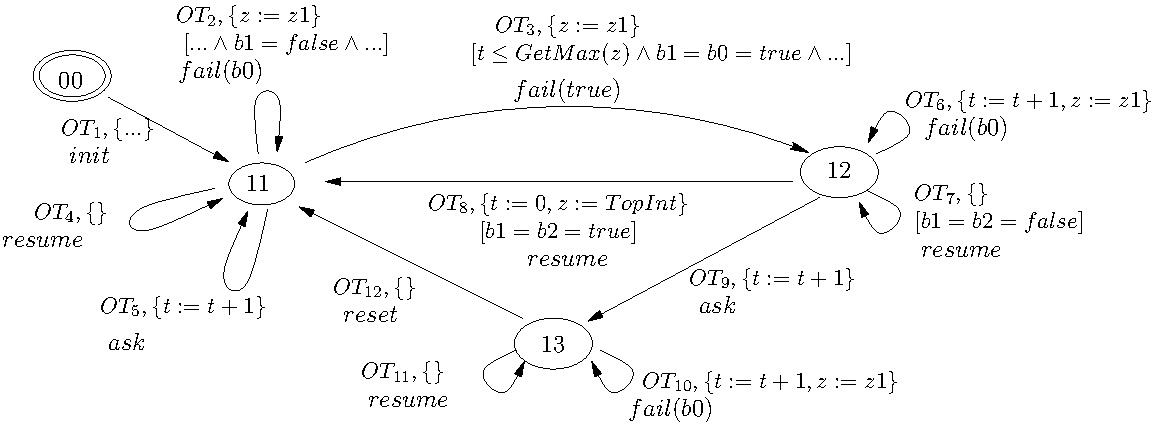
\includegraphics[width=\columnwidth]{TimerOAFullDetailed}
  \caption{The open Automaton of the Failure Monitor Architecture}
  \label{schema:ArchFailure:OA-annex}
\end{figure}


\medskip
\noindent
$  OT_1  = \openrule
{\emptyset, \{t:=0, z:=TopInt, zone:=[minZone,maxZone]\} }
{\ostate{00} \OTarrow{init} \ostate{11}}
$

\medskip    
\noindent
$  OT_2  = \openrule
{\{B\mapsto fail(b0)\},\\
  t<GetMax(z) \land b1=false \land b1=>b0 \land z1= (z \cap (b1?zone;TopInt)+t),\\
  \{z:=z1\} }
{\ostate{11} \OTarrow{fail} \ostate{11}}
$
\medskip
  
\noindent
  $  OT_3  = \openrule
  {\{B\mapsto fail(b0)\},\\
    t<GetMax(z) \land b1=true \land b1=>b0 \land z1= (z \cap (b1?zone;TopInt)+t),\\
    \{z:=z1\} }
  {\ostate{11} \OTarrow{fail} \ostate{12}}
  $
  \medskip

\noindent
  $  OT_4  = \openrule
  {\{B\mapsto resume\},
    b1=false \land b2=false \land b1=b2
    \{\}  }
  {\ostate{11} \OTarrow{resume} \ostate{11}}
  $
  \medskip
  
\noindent
  $  OT_5  = \openrule
  {\{E\mapsto ask\},
    t \in z,
    \{t:=t+1\}  }
  {\ostate{11} \OTarrow{ask} \ostate{11}}
  $
  \medskip

\noindent
  $  OT_6  = \openrule
  {\{B\mapsto fail(b0)\},\\
    t<GetMax(z) \land b1=false \land b1=>b0 \land z1=(z \cap (b1?zone;TopInt)+t),\\
    \{t:=t+1, z:=z1\} }
  {\ostate{12} \OTarrow{fail} \ostate{12}}
  $
  \medskip

\noindent
  $  OT_7  = \openrule
  {\{B\mapsto resume\},
    b1=false \land b2=false \land b1=b2,
    \{\} }
  {\ostate{12} \OTarrow{resume} \ostate{12}}
  $
  \medskip

\noindent
  $  OT_8  = \openrule
  {\{B\mapsto resume\},
    b1=true \land b2=true \land b1=b2, 
    \{t:=0, z:=TopInt\} }
  {\ostate{12} \OTarrow{resume} \ostate{11}}
  $
  \medskip

\noindent
  $  OT_9  = \openrule
  {\{E\mapsto ask\},
    t \in z,
    \{t:=t+1\} }
  {\ostate{12} \OTarrow{ask} \ostate{13}}
  $
  \medskip

\noindent
  $  OT_{10}  = \openrule
  {\{B\mapsto fail(b0)\},\\
    t<GetMax(z) \land b1=false \land b1=>b0 \land z1=(z \cap (b1?zone;TopInt)+t),\\
    \{t:=t+1, z:=z1\} }
  {\ostate{13} \OTarrow{fail} \ostate{13}}
  $
  \medskip

\noindent
  $  OT_{11}  = \openrule
  {\{B\mapsto resume\},
    b1=false \land b2=false \land b1=b2,
    \{\} }
  {\ostate{13} \OTarrow{resume} \ostate{13}}
  $
  \medskip

\noindent
  $  OT_{12}  = \openrule
  {\{E\mapsto reset\},
    true,
    \{\} }
  {\ostate{13} \OTarrow{reset} \ostate{11}}
  $

  \medskip

  \subsubsection{Properties}

  In Fig. \ref{schema:ArchFailure:OA-annex}, you can see that some
  properties from appendix \app{properties} do not hold.

  In particular, the first safety property \eq{prop:reset:can}:
  \begin{equation*}
    \AG \bigl(\PortFail(true) \rightarrow \EU[]{\lnot \PortFail(true)}{\PortReset}\bigr).
  \end{equation*}
is not true, because the $OT_2$ loop on state $\ostate{11}$ stays in
state 11 where you need another $\PortFail(true)$ before enabling a
reset. This is because without priorities we can have an
activity on the dandling ``fail'' port without synchronising with the
others, even if they are available.
  
This can be sloved by the version with the Max Progress encoding.
This modifies both the pLTS transitions, and the synchronisation
vectors, as shown below:
 

\small\begin{verbatim}
SV0: <tick(z, t, z1), fail(zone, bf, b1), fail(b0), _> --> fail(b0),
         [(b1=>b0)/\((bf/\b0)=>b1)/\(z1=(z |Intersection| ((b1?zone:TopInt)+t)))]
SV1: <cancel(bc, b1), resume(br, b2), resume, _>-->resume, (b1=b2)/\((bc/\br)=>(b1/\b2))
SV2: <timeout, timeout, _, ask> --> ask
SV3: <_, reset, _, reset> --> reset
SV4: <init, init, _, _> --> init

pLTS: Timer
- Transition: t0---init-->t1, { t := 0 z := TopInt}
- Transition: t1---tick(z, t, z1)-->t1, [t<(GET_MAX z)], { t := t+1 z := z1}
- Transition: t1---cancel(true, false)-->t1, {}
- Transition: t1---cancel(true, true)-->t1, { t := 0 z := TopInt}
- Transition: t1---timeout-->t1, [t in z], { t := 0 z := TopInt}
pLTS: Control
- Transition: s0---init-->s1, { zone := minZone,maxZone}
- Transition: s1---timeout-->s1, {}
- Transition: s1---resume(false, false)-->s1, {}
- Transition: s1---fail(zone, true, false)-->s1, {}
- Transition: s1---fail(zone, true, true)-->s2, {}
- Transition: s2---fail(zone, false, false)-->s2, {}
- Transition: s2---resume(true, false)-->s2, {}
- Transition: s2---resume(true, true)-->s1, {}
- Transition: s2---timeout-->s3, {}
- Transition: s3---fail(zone, false, false)-->s3, {}
- Transition: s3---resume(false, false)-->s3, {}
- Transition: s3---reset-->s1, {}
\end{verbatim}

  The new OA is shown in figure \ref{schema:ArchFailure:OA-MaxProgress}.

  \begin{figure}[t]
  \centering
  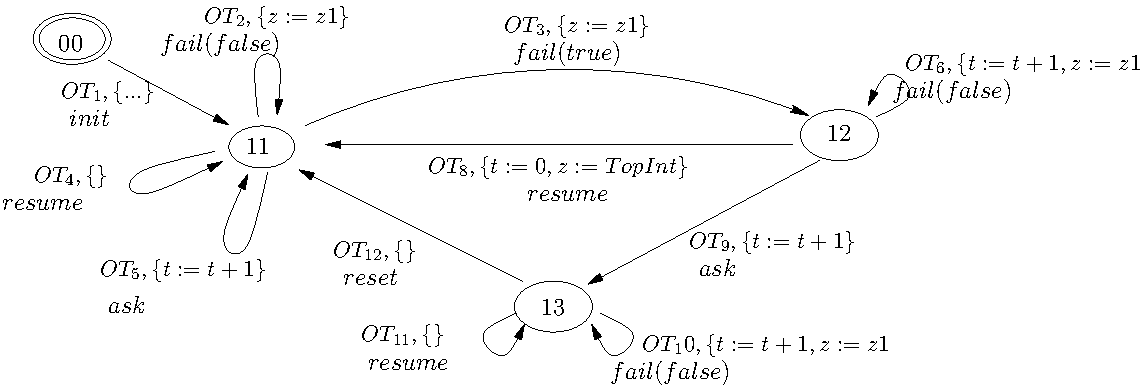
\includegraphics[width=\columnwidth]{TimerOAMaxProgress}
  \caption{The open Automaton of the Failure Monitor Architecture,
    with Maximal Progress}
  \label{schema:ArchFailure:OA-MaxProgress}
\end{figure}

\begin{itemize}
\item $OT_2$ and $OT_{10}$ have changed because $b0=true$ is no longer possible
\item $OT_7$ has disappeared because it is now unsat.
\end{itemize}

  Here we give the detail of the modification of $OT_2$:

\begin{verbatim}
  {t1---tick(z, t, z1)-->t1, s1---fail(zone, true, false)-->s1},
  {B|->fail(b0:sva_SV0)},
    [(t<(GET_MAX z))
     /\((tick(z, t, z1))=(tick(z:sva_SV0, t:sva_SV0, z1:sva_SV0)))
     /\((fail(zone, true, false))=(fail(zone:sva_SV0, bf:sva_SV0, b1:sva_SV0)))
     /\(b1:sva_SV0=>b0:sva_SV0)
     /\((bf:sva_SV0/\b0:sva_SV0)=>b1:sva_SV0)
     /\(z1:sva_SV0=(z:sva_SV0 |Intersection|
                    ((b1:sva_SV0?(zone:sva_SV0):(TopInt))+t:sva_SV0)))],
 {t := t+1, z := z1}
OT:2 ------------------------------------------------------------
     <t1_s1>-----fail(b0:sva_SV0)----><t1_s1>
\end{verbatim}

As \verb|bf| is true, and \verb|b1| is false, the predicate fragment
\verb|((bf/\b0)=>b1)| imposes that \verb|b0| is false.

\subsubsection{Scaling-up: composing architectures}

\medskip

Here is the code of the corresponding composed pNet:
\noteEMin{Il faudrait (mais a-t-on le temps?): faire un dessin de la
  composition au niveau BIP, et au niveau pNet. Un resultat brut, vaguement
  correct, montre 37 OTs, modulo les petites questions de mon mail de
  mercredi midi...}
  
  
\todoSBin{Ecrire les proprietes qu'il doit verifier... ? }


\medskip
\begin{verbatim}
SV0: <tick(z, t, z1), fail(zone1, b11), fail(zone2, b12), fail1(b01), fail2(b02), _> 
     --> fail(b01, b02), 
     [(z1 = z |Intersection| ((b11?zone1:TopInt)+t) |Intersection| ((b12?zone2:TopInt)+t))
      /\(b11=>b01)/\(b12=>b02)]
SV1: <cancel(b1), resume(b21), resume(b22), resume1, resume2, _>-->resume, 
     [(b1=b21)/\(b1=b22)]
SV2: <timeout, timeout, timeout, _, _, ask>-->ask
SV3: <_, reset, reset, _, _, reset>-->reset
SV4: <init, init, init, _, _, _>-->init

pLTS: Timer
- Transition: t0---init-->t1, { t := 0 z := TopInt}
- Transition: t1---tick(z, t, z1)-->t1, [t<(GET_MAX z)], { t := t+1 z := z1}
- Transition: t1---cancel(false)-->t1, {}
- Transition: t1---cancel(true)-->t1, { t := 0 z := TopInt}
- Transition: t1---timeout-->t1, [t in z], { t := 0 z := TopInt}

pLTS: FC1
- Transition: s0---init-->s1, { zone1 := minZone1,maxZone1}
- Transition: s1---timeout-->s1, {}
- Transition: s1---resume(false)-->s1, {}
- Transition: s1---fail(zone1, false)-->s1, {}
- Transition: s1---fail(zone1, true)-->s2, {}
- Transition: s2---fail(zone1, false)-->s2, {}
- Transition: s2---resume(false)-->s2, {}
- Transition: s2---resume(true)-->s1, {}
- Transition: s2---timeout-->s3, {}
- Transition: s3---fail(zone1, false)-->s3, {}
- Transition: s3---timeout-->s3, {}
- Transition: s3---resume(false)-->s3, {}
- Transition: s3---reset-->s1, {}

pLTS: FC2
- Transition: s0---init-->s1, { zone2 := minZone2,maxZone2}
- Transition: s1---timeout-->s1, {}
- Transition: s1---resume(false)-->s1, {}
- Transition: s1---fail(zone2, false)-->s1, {}
- Transition: s1---fail(zone2, true)-->s2, {}
- Transition: s2---fail(zone2, false)-->s2, {}
- Transition: s2---resume(false)-->s2, {}
- Transition: s2---resume(true)-->s1, {}
- Transition: s2---timeout-->s3, {}
- Transition: s3---fail(zone2, false)-->s3, {}
- Transition: s3---timeout-->s3, {}
- Transition: s3---resume(false)-->s3, {}
- Transition: s3---reset-->s1, {}

INFO  BIPArchFailureTimerMaxV4X2 - Total: 37 SATISFIABLE OTs
INFO  BIPArchFailureTimerMaxV4X2 -        3136 UNSATISFIABLE OTs
INFO  BIPArchFailureTimerMaxV4X2 - Total Time: 9111 ms
\end{verbatim}

\bigskip
Fig. \ref{schema:ArchFailure:OA-TimerV4X2} shows the open automata of
this composed architecture.
Note that e..g. the open transition labelled ``$fail(*,tt)$'' stands for
``$fail(b01,b02)$'', where  $b01'$ can be arbitrarily true or
false. As in the previous case, this is because we have not use here
the Max Progress hypothesis, otherwise all the ``*'' in the figure
should be replaced by ``$ff$''.

  \begin{figure}[h]
  \centering
  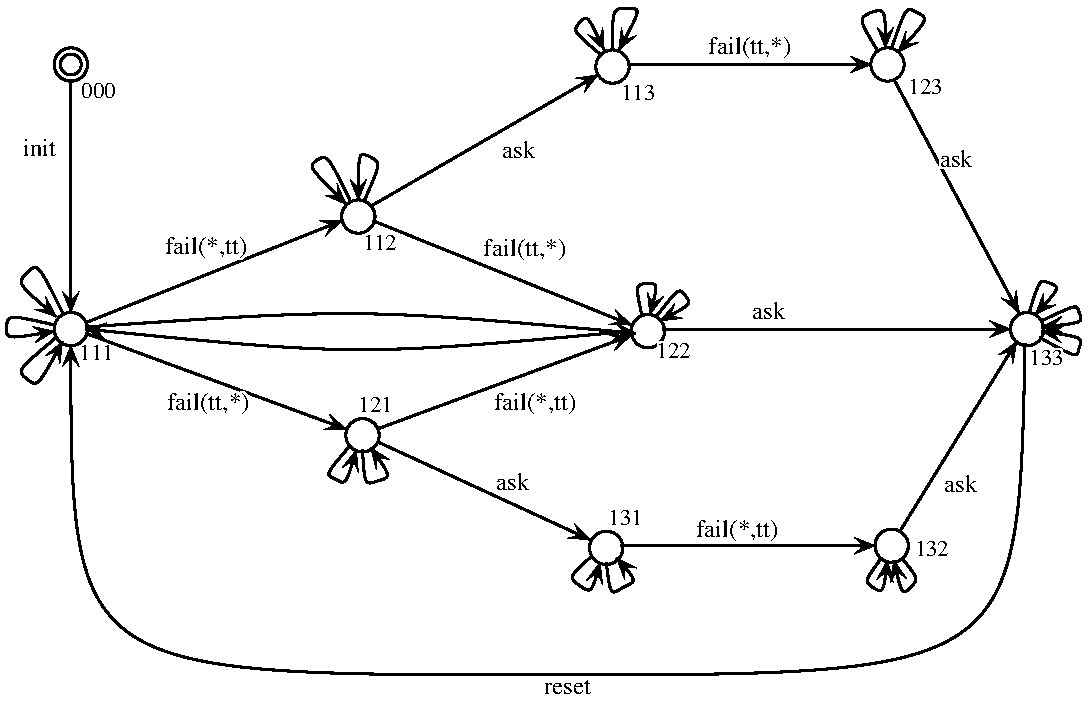
\includegraphics[width=0.8\columnwidth]{TimerV4X2}
  \caption{The open Automaton of the composed system}
  \label{schema:ArchFailure:OA-TimerV4X2}
\end{figure}

\end{document}
